% !TeX root = slides.tex
\section{Predictive Checks}

\subsection{Recommended References}
\begin{frame}{Predictive Checks - Recommended References}
	\begin{vfilleditems}
		\item \textcite{gelman2013bayesian} - Chapter 6: Model checking
		\item \textcite{mcelreath2020statistical} - Chapter 4: Geocentric Models
		\item \textcite{gelman2020regression}:
		\begin{vfilleditems}
			\item Chapter 6: Background on regression modeling
			\item Chapter 11: Assumptions, diagnostics, and model evaluation
		\end{vfilleditems}
		\item \textcite{gelmanBayesianWorkflow2020}
	\end{vfilleditems}
\end{frame}

\subsection{All models are wrong}
\begin{frame}{All models are wrong}
	\begin{columns}
		\begin{column}{0.8\textwidth}
			\begin{quotation}
				All models are wrong but some are useful
			\end{quotation}
			\vfill
			\textcite{boxScienceStatistics1976}
		\end{column}
		\begin{column}{0.2\textwidth}
			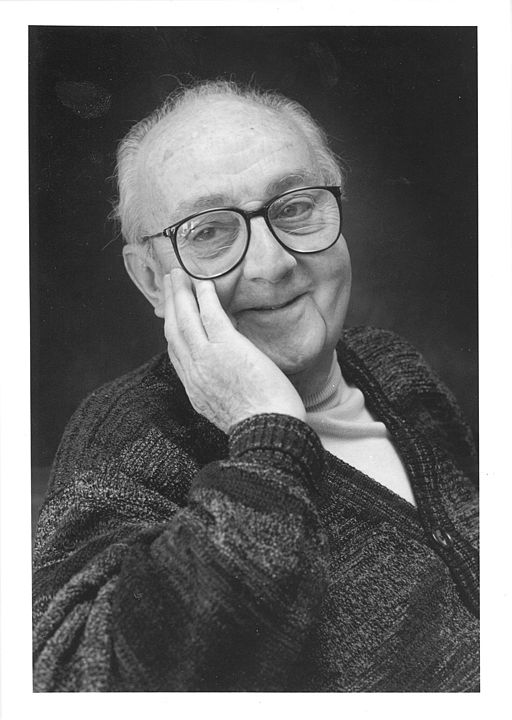
\includegraphics[width=0.9\columnwidth]{george_box.jpg}
		\end{column}
	\end{columns}
\end{frame}

\subsection{Bayesian Workflow}
\begin{frame}{Bayesian Workflow\footnote{based on \textcite{gelmanBayesianWorkflow2020}}}
	\centering
	\begin{tikzpicture}[
			scale=0.8,
			transform shape, thick,
			every node/.style={text width=3.5cm, align=center},
			constructs/.style = {draw,
					ellipse,
					minimum width=4cm,
					minimum height=2cm}
		]
		\node[constructs] (Model) {Model Specification};
		\node[constructs] [right = of Model] (Prior) {Prior Elicitation};
		\node[constructs] [right = of Prior] (Posterior) {Posterior Inference};
		\draw [<->, line width=1pt] (Model) to [out=45,in=135] node[above] {\textit{Prior Predictive Check}} (Prior);
		%\draw [->, line width=1pt] (Prior) to [out=225,in=315] {} (Model);
		\draw [<->, line width=1pt] (Prior) to [out=45,in=135] node[above] {\textit{Posterior Predictive Check}} (Posterior);
		%\draw [->, line width=1pt] (Posterior) to [out=225,in=315] {} (Prior);
	\end{tikzpicture}
\end{frame}

\begin{frame}{Bayesian Workflow\footnote{
			adapted from \href{https://github.com/elizavetasemenova}
			{Elizaveta Semenova}.}}
	\begin{vfilleditems}
		\item Understand the domain and problem.
		\item Formulate the model mathematically.
		\item Implement model, test, and debug.
		\item Perform prior predictive checks.
		\item Fit the model.
		\item Assess convergence diagnostics.
		\item Perform posterior predictive checks.
		\item Improve the model iteratively: from baseline to complex and computationally efficient models.
	\end{vfilleditems}

\end{frame}

\begin{frame}{Actual Bayesian Workflow}
	\centering
	\begin{figure}
		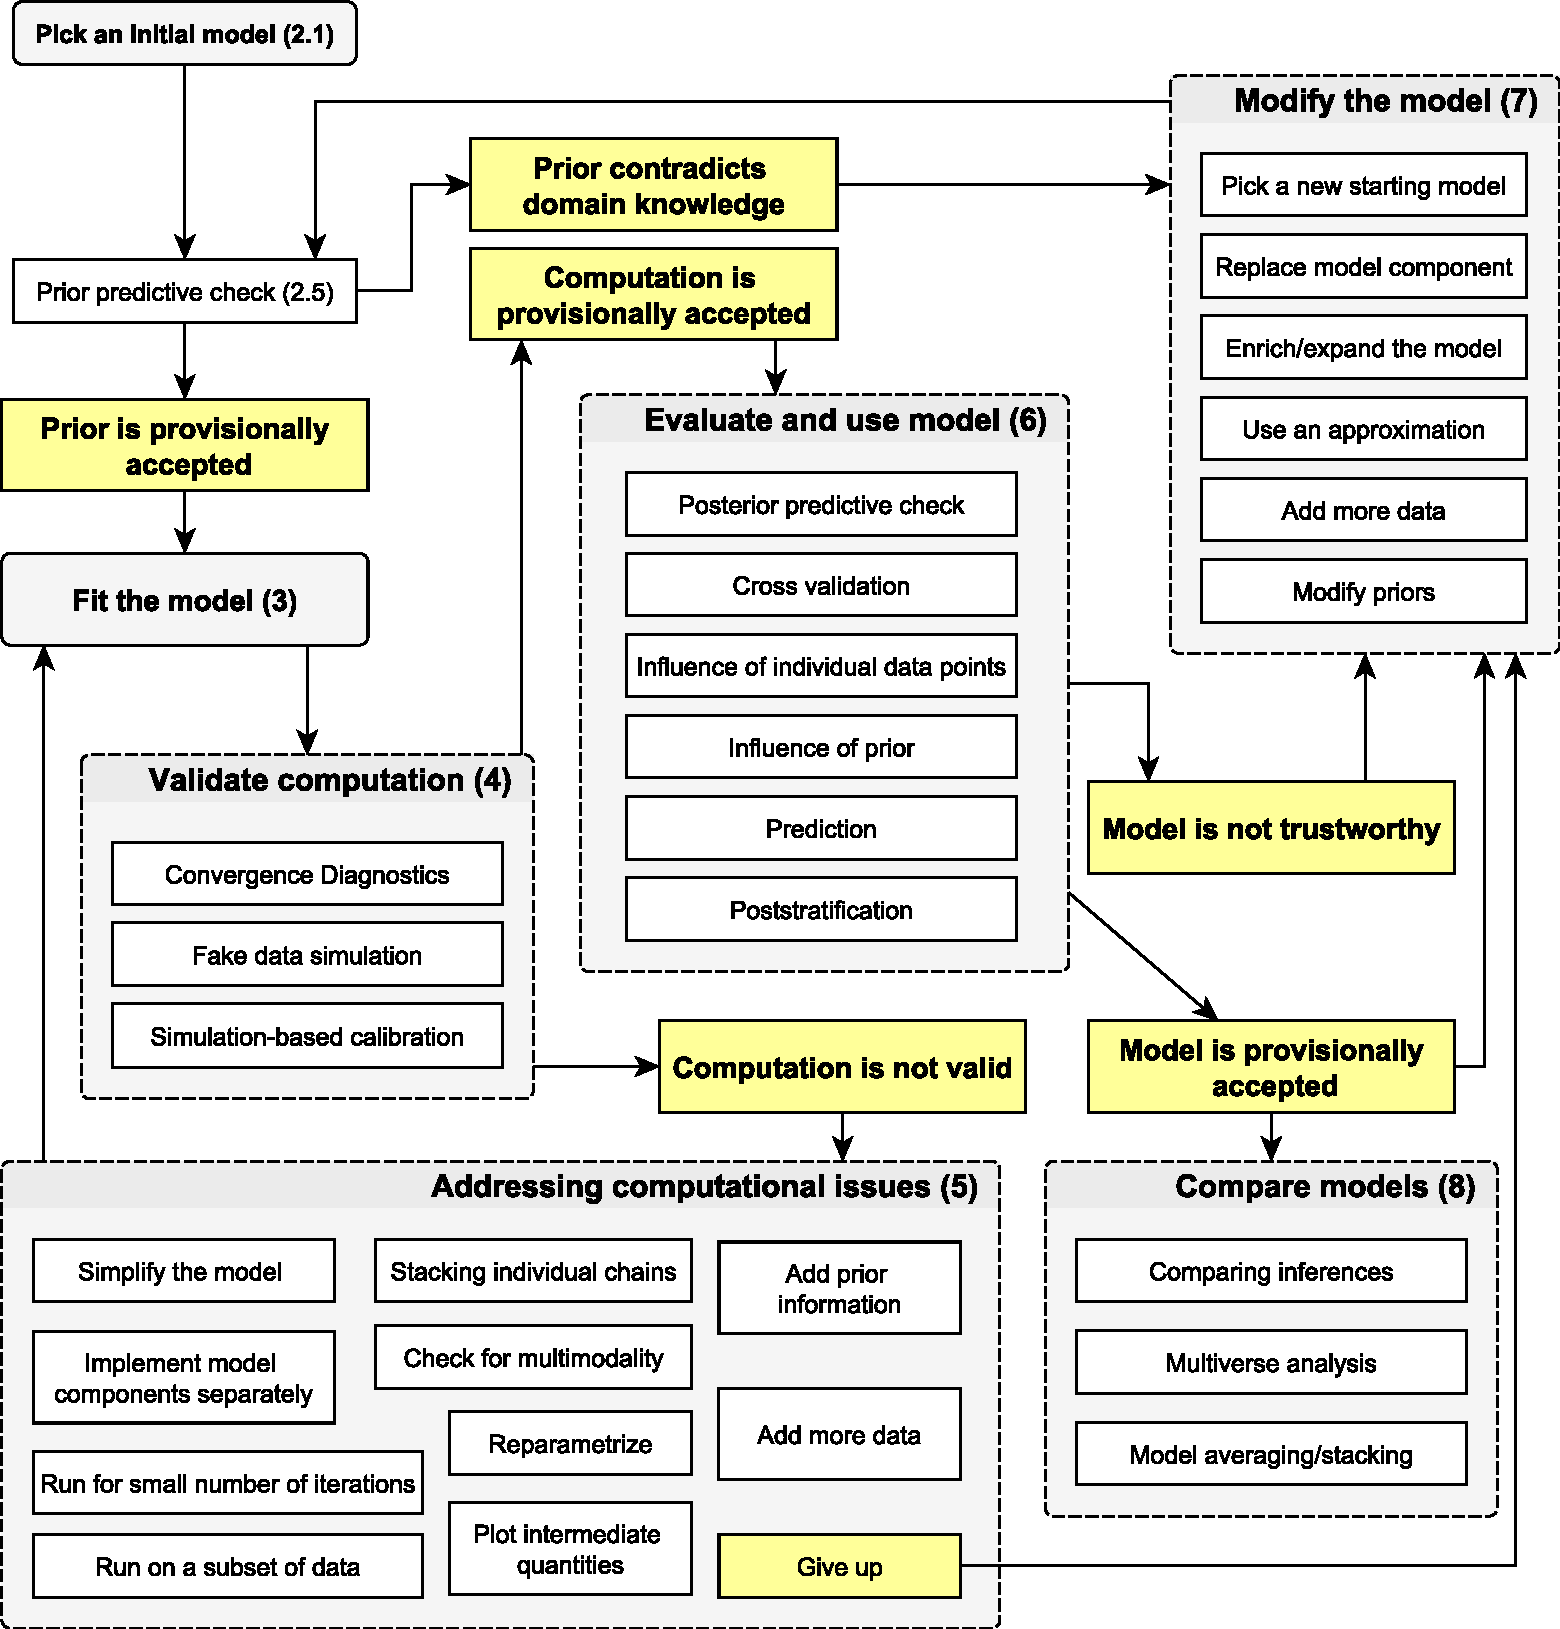
\includegraphics[height=0.75\textheight]{workflow_overview.pdf}
		\caption{Bayesian workflow by \textcite{gelmanBayesianWorkflow2020}}
	\end{figure}
\end{frame}

\begin{frame}{Not a ``new ideia''...}
	\centering
	\begin{figure}
		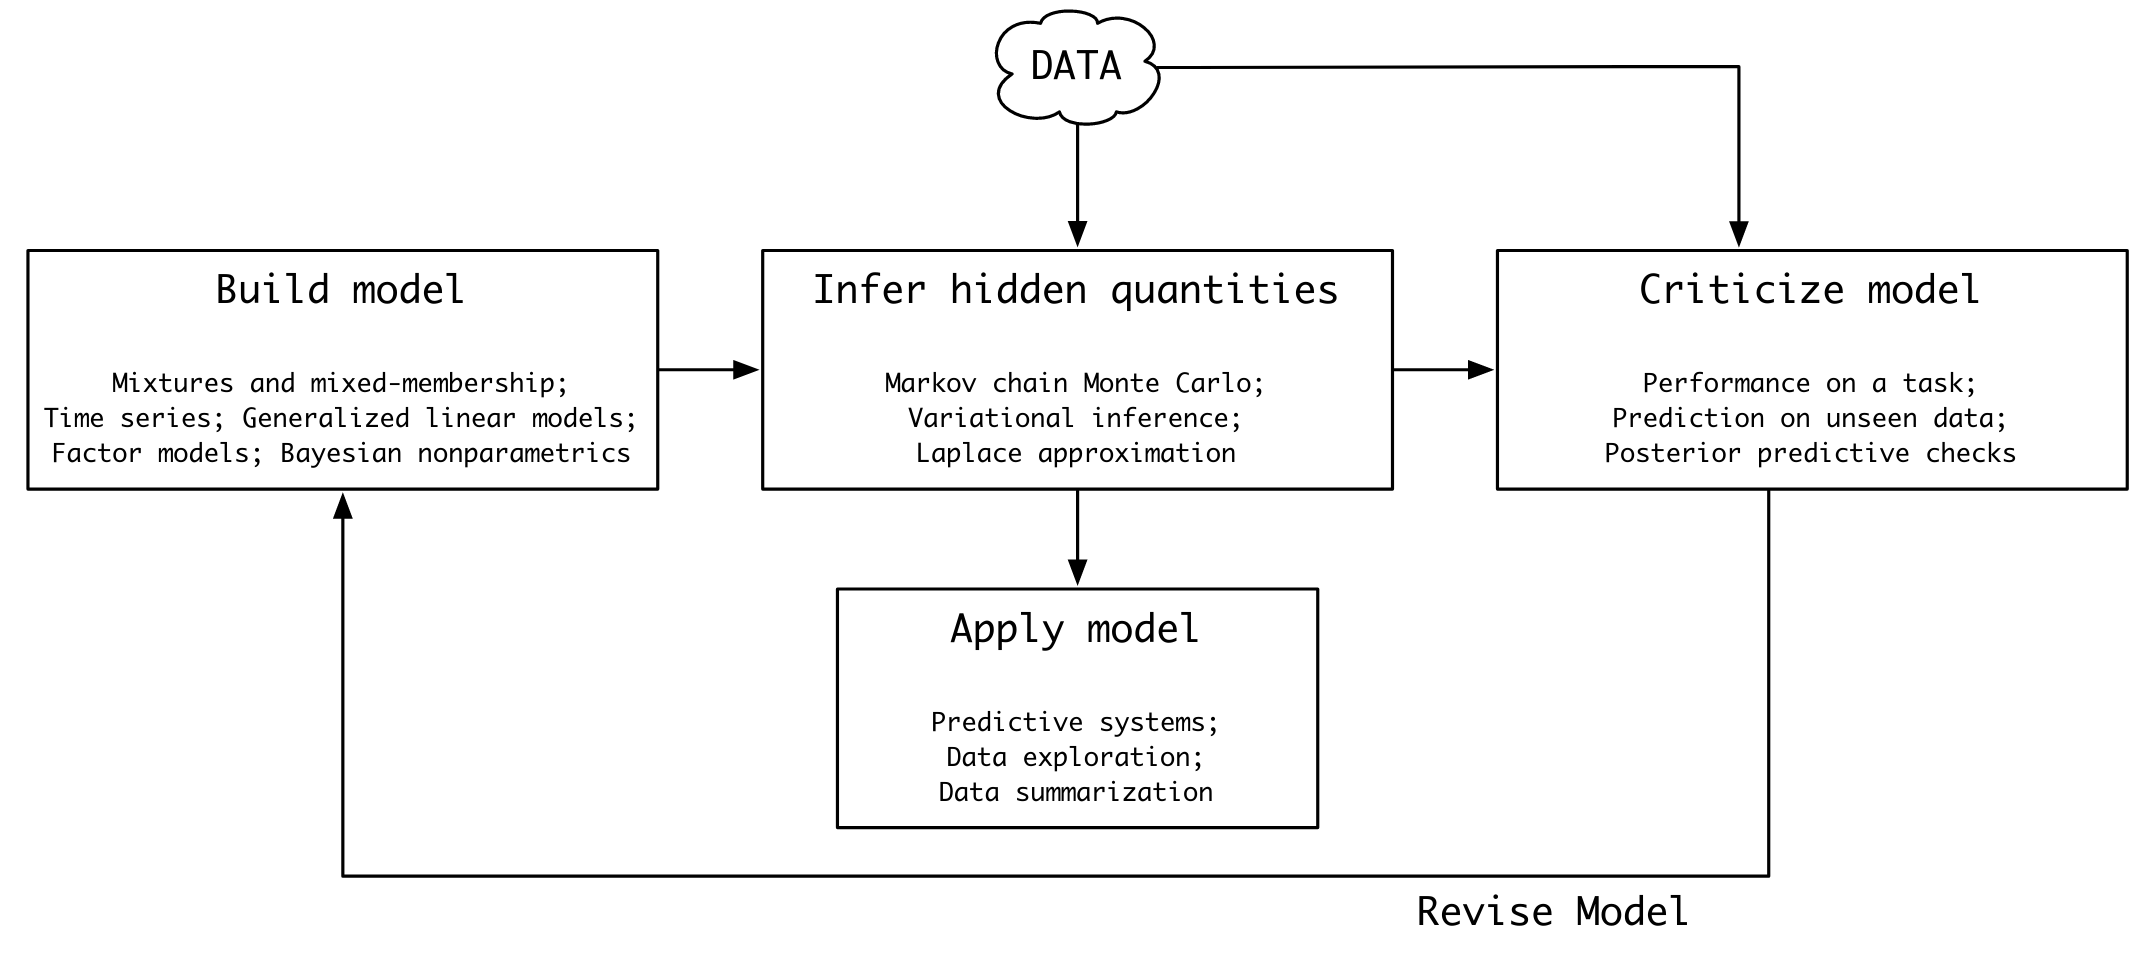
\includegraphics[width=0.8\textwidth]{box_loop.png}
		\caption{Box's Loop from \textcite{boxScienceStatistics1976}
			but taken from \textcite{Blei_Workflow2014}}
	\end{figure}
\end{frame}

\subsection{Prior Predictive Check}
\begin{frame}{Prior Predictive Check}
	Before we feed data into our model,
	we need to check all of our priors.
	\vfill
	In a very simple way, it consists in simulate parameter values based on
	prior distribution without conditioning on any data or employing any
	likelihood function.
	\vfill
	Independent of the level of information specified in the priors,
	it is always important to perform a prior sensitivity analysis
	in order to have a deep understanding of the prior influence onto
	the posterior.
\end{frame}

\subsection{Posterior Predictive Check}
\begin{frame}{Posterior Predictive Check}
	We need to make sure that the posterior distribution of $\mathbf{y}$,
	namely $\boldsymbol{\tilde{y}}$,
	can capture all the nuances of the real distribution density/mass of $\mathbf{y}$.
	\vfill
	This procedure is called \textbf{posterior predictive check},
	and it is generally carried on by a visual inspection\footnote{
		we also perform mathematical/exact inspections,
		see the section on \textit{Model Comparison}.}
	of the real density/mass of $\mathbf{y}$ against generated samples
	of $\mathbf{y}$ by the Bayesian model.
	\vfill
	The purpose is to compare the histogram of the dependent variable $\mathbf{y}$
	against the histograms of simulated dependent variables $\mathbf{y}_{\text{rep}}$
	by the model after parameter inference.\
	The ideia is that the real and simulated histograms blend together and
	we do not observer any divergences.
\end{frame}

\begin{frame}{Examples of Posterior Predictive Checks}
	% library(brms)
	% library(ggplot2)
	% library(ggdark)
	% library(bayesplot)
	% library(tikzDevice)
	% theme_set(dark_theme_light())
	% bayesplot_theme_set(dark_theme_light())
	% brms_fit <- brm(mpg ~ wt + am, data = mtcars)
	% tikz(file = "slides/images/pp_check_brms.tex")
	% pp_check(brms_fit, nreps = 10, seed = 123)
	% dev.off()
	% tikz(file = "slides/images/pp_check_brms_ecdf.tex")
	% pp_check(brms_fit, nreps = 10, seed = 123, type = "ecdf_overlay")
	% dev.off()
	\begin{columns}
		\begin{column}{0.5\textwidth}
			\begin{figure}
				\centering
				\resizebox{0.8\columnwidth}{!}{% Created by tikzDevice version 0.12.3.1 on 2021-06-01 06:51:26
% !TEX encoding = UTF-8 Unicode
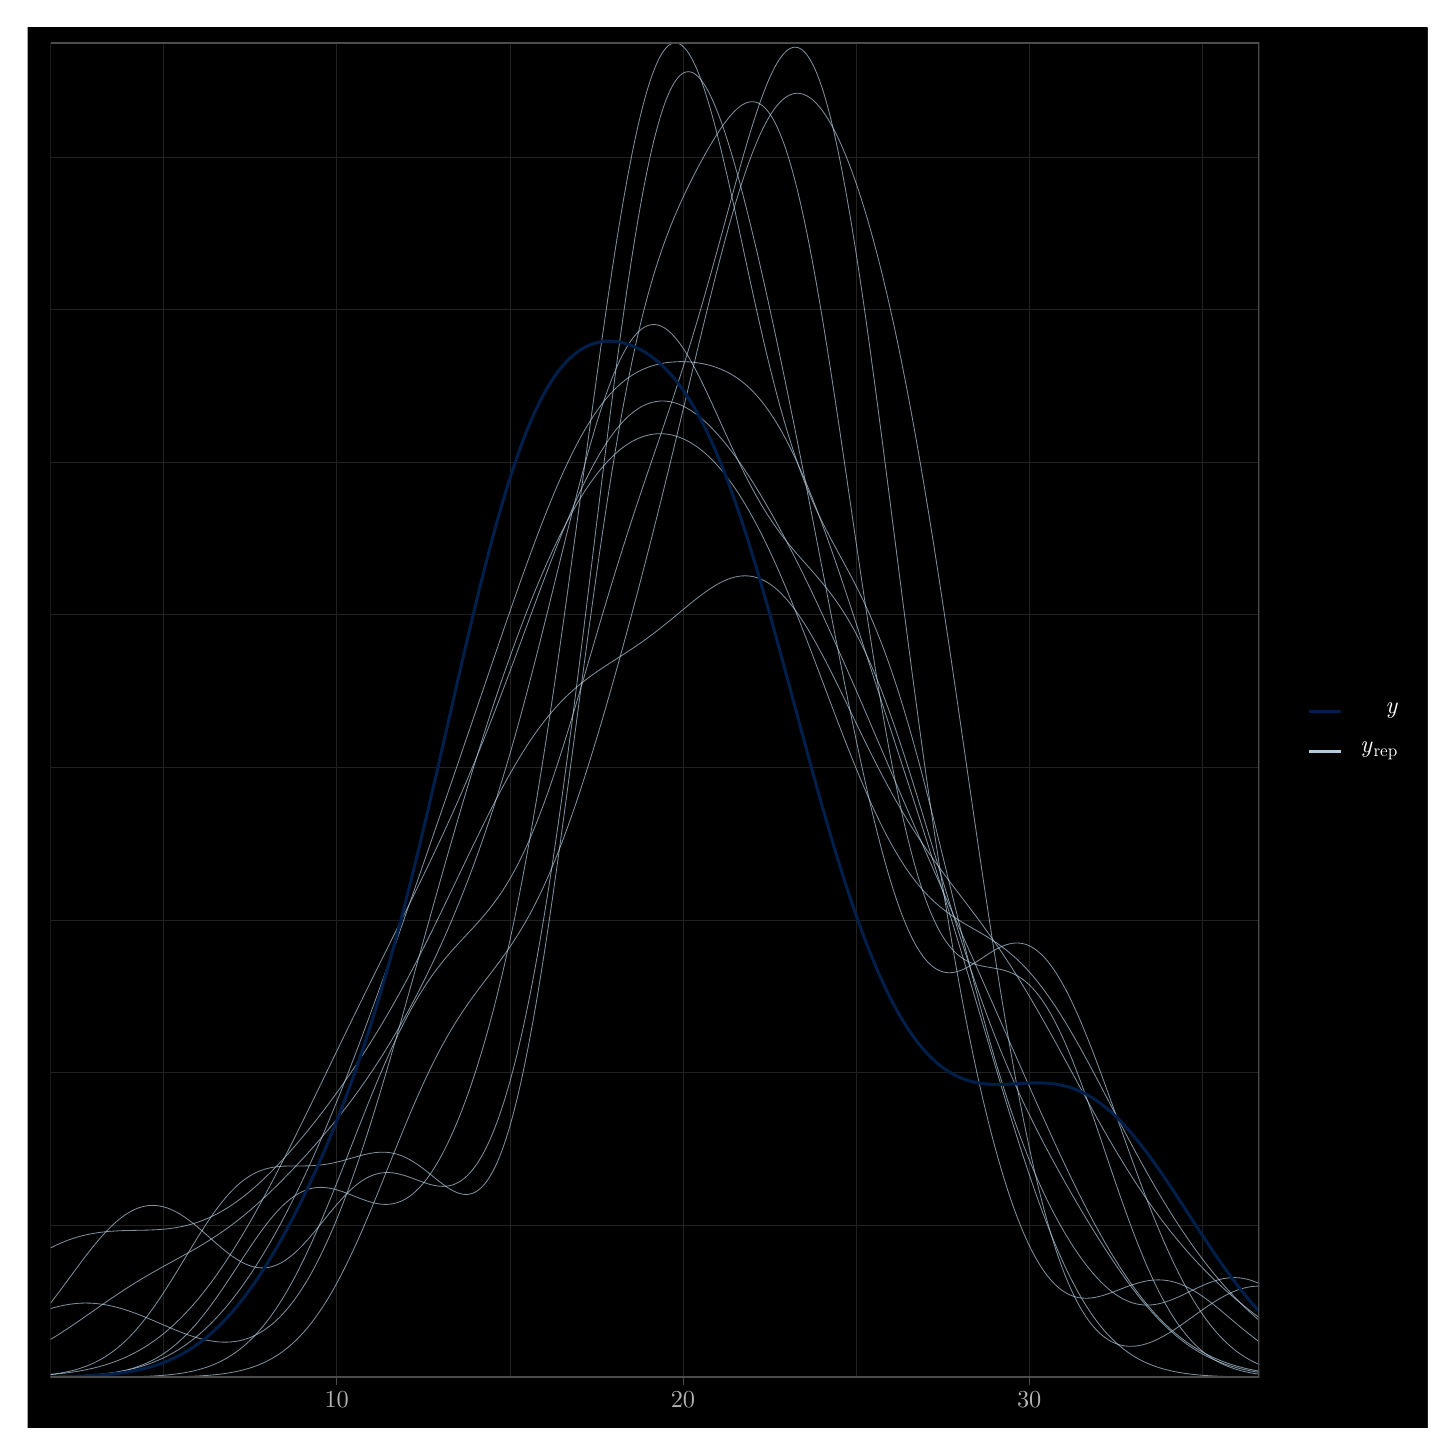
\begin{tikzpicture}[x=1pt,y=1pt]
\definecolor{fillColor}{RGB}{255,255,255}
\path[use as bounding box,fill=fillColor,fill opacity=0.00] (0,0) rectangle (505.89,505.89);
\begin{scope}
\path[clip] (  0.00,  0.00) rectangle (505.89,505.89);
\definecolor{drawColor}{RGB}{0,0,0}
\definecolor{fillColor}{RGB}{0,0,0}

\path[draw=drawColor,line width= 0.6pt,line join=round,line cap=round,fill=fillColor] (  0.00,  0.00) rectangle (505.89,505.89);
\end{scope}
\begin{scope}
\path[clip] (  8.25, 18.22) rectangle (445.03,500.39);
\definecolor{fillColor}{RGB}{0,0,0}

\path[fill=fillColor] (  8.25, 18.22) rectangle (445.03,500.39);
\definecolor{drawColor}{gray}{0.13}

\path[draw=drawColor,line width= 0.1pt,line join=round] (  8.25, 73.33) --
	(445.03, 73.33);

\path[draw=drawColor,line width= 0.1pt,line join=round] (  8.25,183.56) --
	(445.03,183.56);

\path[draw=drawColor,line width= 0.1pt,line join=round] (  8.25,293.79) --
	(445.03,293.79);

\path[draw=drawColor,line width= 0.1pt,line join=round] (  8.25,404.01) --
	(445.03,404.01);

\path[draw=drawColor,line width= 0.1pt,line join=round] ( 49.12, 18.22) --
	( 49.12,500.39);

\path[draw=drawColor,line width= 0.1pt,line join=round] (174.24, 18.22) --
	(174.24,500.39);

\path[draw=drawColor,line width= 0.1pt,line join=round] (299.35, 18.22) --
	(299.35,500.39);

\path[draw=drawColor,line width= 0.1pt,line join=round] (424.47, 18.22) --
	(424.47,500.39);

\path[draw=drawColor,line width= 0.3pt,line join=round] (  8.25,128.45) --
	(445.03,128.45);

\path[draw=drawColor,line width= 0.3pt,line join=round] (  8.25,238.67) --
	(445.03,238.67);

\path[draw=drawColor,line width= 0.3pt,line join=round] (  8.25,348.90) --
	(445.03,348.90);

\path[draw=drawColor,line width= 0.3pt,line join=round] (  8.25,459.13) --
	(445.03,459.13);

\path[draw=drawColor,line width= 0.3pt,line join=round] (111.68, 18.22) --
	(111.68,500.39);

\path[draw=drawColor,line width= 0.3pt,line join=round] (236.80, 18.22) --
	(236.80,500.39);

\path[draw=drawColor,line width= 0.3pt,line join=round] (361.91, 18.22) --
	(361.91,500.39);
\definecolor{drawColor}{RGB}{179,205,224}

\path[draw=drawColor,draw opacity=0.70,line width= 0.3pt,line join=round] (  8.25, 18.31) --
	(  8.68, 18.32) --
	(  9.10, 18.33) --
	(  9.53, 18.33) --
	(  9.96, 18.34) --
	( 10.38, 18.35) --
	( 10.81, 18.35) --
	( 11.24, 18.36) --
	( 11.67, 18.37) --
	( 12.09, 18.38) --
	( 12.52, 18.39) --
	( 12.95, 18.40) --
	( 13.37, 18.41) --
	( 13.80, 18.42) --
	( 14.23, 18.43) --
	( 14.65, 18.44) --
	( 15.08, 18.46) --
	( 15.51, 18.47) --
	( 15.94, 18.49) --
	( 16.36, 18.50) --
	( 16.79, 18.52) --
	( 17.22, 18.53) --
	( 17.64, 18.55) --
	( 18.07, 18.57) --
	( 18.50, 18.59) --
	( 18.92, 18.61) --
	( 19.35, 18.63) --
	( 19.78, 18.65) --
	( 20.20, 18.68) --
	( 20.63, 18.70) --
	( 21.06, 18.73) --
	( 21.49, 18.76) --
	( 21.91, 18.79) --
	( 22.34, 18.82) --
	( 22.77, 18.85) --
	( 23.19, 18.88) --
	( 23.62, 18.91) --
	( 24.05, 18.95) --
	( 24.47, 18.99) --
	( 24.90, 19.03) --
	( 25.33, 19.07) --
	( 25.76, 19.11) --
	( 26.18, 19.16) --
	( 26.61, 19.20) --
	( 27.04, 19.25) --
	( 27.46, 19.30) --
	( 27.89, 19.36) --
	( 28.32, 19.41) --
	( 28.74, 19.47) --
	( 29.17, 19.53) --
	( 29.60, 19.59) --
	( 30.02, 19.66) --
	( 30.45, 19.72) --
	( 30.88, 19.79) --
	( 31.31, 19.87) --
	( 31.73, 19.94) --
	( 32.16, 20.02) --
	( 32.59, 20.11) --
	( 33.01, 20.19) --
	( 33.44, 20.28) --
	( 33.87, 20.37) --
	( 34.29, 20.47) --
	( 34.72, 20.57) --
	( 35.15, 20.67) --
	( 35.58, 20.78) --
	( 36.00, 20.89) --
	( 36.43, 21.00) --
	( 36.86, 21.12) --
	( 37.28, 21.25) --
	( 37.71, 21.37) --
	( 38.14, 21.50) --
	( 38.56, 21.64) --
	( 38.99, 21.78) --
	( 39.42, 21.93) --
	( 39.84, 22.08) --
	( 40.27, 22.23) --
	( 40.70, 22.39) --
	( 41.13, 22.56) --
	( 41.55, 22.73) --
	( 41.98, 22.91) --
	( 42.41, 23.09) --
	( 42.83, 23.28) --
	( 43.26, 23.47) --
	( 43.69, 23.67) --
	( 44.11, 23.87) --
	( 44.54, 24.08) --
	( 44.97, 24.30) --
	( 45.40, 24.52) --
	( 45.82, 24.75) --
	( 46.25, 24.99) --
	( 46.68, 25.23) --
	( 47.10, 25.48) --
	( 47.53, 25.74) --
	( 47.96, 26.00) --
	( 48.38, 26.27) --
	( 48.81, 26.54) --
	( 49.24, 26.83) --
	( 49.66, 27.12) --
	( 50.09, 27.42) --
	( 50.52, 27.72) --
	( 50.95, 28.03) --
	( 51.37, 28.35) --
	( 51.80, 28.68) --
	( 52.23, 29.02) --
	( 52.65, 29.36) --
	( 53.08, 29.71) --
	( 53.51, 30.07) --
	( 53.93, 30.43) --
	( 54.36, 30.81) --
	( 54.79, 31.19) --
	( 55.22, 31.58) --
	( 55.64, 31.97) --
	( 56.07, 32.38) --
	( 56.50, 32.79) --
	( 56.92, 33.21) --
	( 57.35, 33.64) --
	( 57.78, 34.07) --
	( 58.20, 34.52) --
	( 58.63, 34.97) --
	( 59.06, 35.43) --
	( 59.48, 35.90) --
	( 59.91, 36.37) --
	( 60.34, 36.85) --
	( 60.77, 37.34) --
	( 61.19, 37.84) --
	( 61.62, 38.34) --
	( 62.05, 38.86) --
	( 62.47, 39.37) --
	( 62.90, 39.90) --
	( 63.33, 40.43) --
	( 63.75, 40.97) --
	( 64.18, 41.52) --
	( 64.61, 42.07) --
	( 65.04, 42.63) --
	( 65.46, 43.20) --
	( 65.89, 43.77) --
	( 66.32, 44.35) --
	( 66.74, 44.93) --
	( 67.17, 45.52) --
	( 67.60, 46.12) --
	( 68.02, 46.72) --
	( 68.45, 47.32) --
	( 68.88, 47.93) --
	( 69.30, 48.55) --
	( 69.73, 49.17) --
	( 70.16, 49.79) --
	( 70.59, 50.42) --
	( 71.01, 51.05) --
	( 71.44, 51.68) --
	( 71.87, 52.32) --
	( 72.29, 52.96) --
	( 72.72, 53.61) --
	( 73.15, 54.25) --
	( 73.57, 54.90) --
	( 74.00, 55.55) --
	( 74.43, 56.20) --
	( 74.86, 56.85) --
	( 75.28, 57.50) --
	( 75.71, 58.15) --
	( 76.14, 58.81) --
	( 76.56, 59.46) --
	( 76.99, 60.11) --
	( 77.42, 60.76) --
	( 77.84, 61.41) --
	( 78.27, 62.06) --
	( 78.70, 62.71) --
	( 79.12, 63.35) --
	( 79.55, 64.00) --
	( 79.98, 64.64) --
	( 80.41, 65.27) --
	( 80.83, 65.91) --
	( 81.26, 66.53) --
	( 81.69, 67.16) --
	( 82.11, 67.78) --
	( 82.54, 68.39) --
	( 82.97, 69.00) --
	( 83.39, 69.60) --
	( 83.82, 70.20) --
	( 84.25, 70.79) --
	( 84.68, 71.38) --
	( 85.10, 71.96) --
	( 85.53, 72.53) --
	( 85.96, 73.09) --
	( 86.38, 73.64) --
	( 86.81, 74.19) --
	( 87.24, 74.73) --
	( 87.66, 75.26) --
	( 88.09, 75.78) --
	( 88.52, 76.29) --
	( 88.94, 76.79) --
	( 89.37, 77.28) --
	( 89.80, 77.76) --
	( 90.23, 78.22) --
	( 90.65, 78.68) --
	( 91.08, 79.13) --
	( 91.51, 79.57) --
	( 91.93, 79.99) --
	( 92.36, 80.40) --
	( 92.79, 80.80) --
	( 93.21, 81.19) --
	( 93.64, 81.57) --
	( 94.07, 81.93) --
	( 94.49, 82.28) --
	( 94.92, 82.62) --
	( 95.35, 82.95) --
	( 95.78, 83.26) --
	( 96.20, 83.56) --
	( 96.63, 83.85) --
	( 97.06, 84.12) --
	( 97.48, 84.38) --
	( 97.91, 84.63) --
	( 98.34, 84.86) --
	( 98.76, 85.08) --
	( 99.19, 85.29) --
	( 99.62, 85.48) --
	(100.05, 85.66) --
	(100.47, 85.83) --
	(100.90, 85.98) --
	(101.33, 86.12) --
	(101.75, 86.25) --
	(102.18, 86.36) --
	(102.61, 86.46) --
	(103.03, 86.55) --
	(103.46, 86.63) --
	(103.89, 86.69) --
	(104.31, 86.74) --
	(104.74, 86.78) --
	(105.17, 86.80) --
	(105.60, 86.82) --
	(106.02, 86.83) --
	(106.45, 86.82) --
	(106.88, 86.80) --
	(107.30, 86.77) --
	(107.73, 86.73) --
	(108.16, 86.69) --
	(108.58, 86.63) --
	(109.01, 86.56) --
	(109.44, 86.48) --
	(109.87, 86.40) --
	(110.29, 86.31) --
	(110.72, 86.20) --
	(111.15, 86.09) --
	(111.57, 85.98) --
	(112.00, 85.86) --
	(112.43, 85.73) --
	(112.85, 85.59) --
	(113.28, 85.45) --
	(113.71, 85.30) --
	(114.13, 85.15) --
	(114.56, 85.00) --
	(114.99, 84.84) --
	(115.42, 84.68) --
	(115.84, 84.52) --
	(116.27, 84.35) --
	(116.70, 84.18) --
	(117.12, 84.01) --
	(117.55, 83.84) --
	(117.98, 83.67) --
	(118.40, 83.50) --
	(118.83, 83.33) --
	(119.26, 83.16) --
	(119.69, 82.99) --
	(120.11, 82.83) --
	(120.54, 82.67) --
	(120.97, 82.51) --
	(121.39, 82.35) --
	(121.82, 82.20) --
	(122.25, 82.05) --
	(122.67, 81.91) --
	(123.10, 81.77) --
	(123.53, 81.64) --
	(123.95, 81.51) --
	(124.38, 81.40) --
	(124.81, 81.29) --
	(125.24, 81.18) --
	(125.66, 81.09) --
	(126.09, 81.00) --
	(126.52, 80.93) --
	(126.94, 80.86) --
	(127.37, 80.80) --
	(127.80, 80.76) --
	(128.22, 80.72) --
	(128.65, 80.70) --
	(129.08, 80.68) --
	(129.51, 80.68) --
	(129.93, 80.69) --
	(130.36, 80.72) --
	(130.79, 80.75) --
	(131.21, 80.80) --
	(131.64, 80.87) --
	(132.07, 80.94) --
	(132.49, 81.03) --
	(132.92, 81.14) --
	(133.35, 81.26) --
	(133.77, 81.39) --
	(134.20, 81.55) --
	(134.63, 81.71) --
	(135.06, 81.89) --
	(135.48, 82.09) --
	(135.91, 82.31) --
	(136.34, 82.54) --
	(136.76, 82.79) --
	(137.19, 83.05) --
	(137.62, 83.33) --
	(138.04, 83.63) --
	(138.47, 83.95) --
	(138.90, 84.28) --
	(139.33, 84.62) --
	(139.75, 84.99) --
	(140.18, 85.38) --
	(140.61, 85.78) --
	(141.03, 86.20) --
	(141.46, 86.64) --
	(141.89, 87.10) --
	(142.31, 87.57) --
	(142.74, 88.06) --
	(143.17, 88.57) --
	(143.59, 89.10) --
	(144.02, 89.65) --
	(144.45, 90.21) --
	(144.88, 90.79) --
	(145.30, 91.40) --
	(145.73, 92.02) --
	(146.16, 92.65) --
	(146.58, 93.31) --
	(147.01, 93.99) --
	(147.44, 94.68) --
	(147.86, 95.39) --
	(148.29, 96.12) --
	(148.72, 96.86) --
	(149.15, 97.63) --
	(149.57, 98.41) --
	(150.00, 99.21) --
	(150.43,100.03) --
	(150.85,100.87) --
	(151.28,101.73) --
	(151.71,102.60) --
	(152.13,103.49) --
	(152.56,104.40) --
	(152.99,105.33) --
	(153.41,106.27) --
	(153.84,107.24) --
	(154.27,108.22) --
	(154.70,109.22) --
	(155.12,110.24) --
	(155.55,111.28) --
	(155.98,112.33) --
	(156.40,113.41) --
	(156.83,114.50) --
	(157.26,115.60) --
	(157.68,116.74) --
	(158.11,117.88) --
	(158.54,119.05) --
	(158.97,120.23) --
	(159.39,121.43) --
	(159.82,122.65) --
	(160.25,123.89) --
	(160.67,125.16) --
	(161.10,126.43) --
	(161.53,127.73) --
	(161.95,129.05) --
	(162.38,130.38) --
	(162.81,131.74) --
	(163.23,133.12) --
	(163.66,134.51) --
	(164.09,135.93) --
	(164.52,137.36) --
	(164.94,138.82) --
	(165.37,140.30) --
	(165.80,141.79) --
	(166.22,143.32) --
	(166.65,144.85) --
	(167.08,146.41) --
	(167.50,148.00) --
	(167.93,149.61) --
	(168.36,151.23) --
	(168.79,152.88) --
	(169.21,154.55) --
	(169.64,156.25) --
	(170.07,157.96) --
	(170.49,159.71) --
	(170.92,161.47) --
	(171.35,163.26) --
	(171.77,165.07) --
	(172.20,166.90) --
	(172.63,168.76) --
	(173.05,170.65) --
	(173.48,172.56) --
	(173.91,174.49) --
	(174.34,176.45) --
	(174.76,178.43) --
	(175.19,180.44) --
	(175.62,182.47) --
	(176.04,184.54) --
	(176.47,186.62) --
	(176.90,188.73) --
	(177.32,190.87) --
	(177.75,193.03) --
	(178.18,195.22) --
	(178.61,197.44) --
	(179.03,199.68) --
	(179.46,201.95) --
	(179.89,204.25) --
	(180.31,206.57) --
	(180.74,208.92) --
	(181.17,211.30) --
	(181.59,213.70) --
	(182.02,216.13) --
	(182.45,218.58) --
	(182.87,221.07) --
	(183.30,223.57) --
	(183.73,226.10) --
	(184.16,228.67) --
	(184.58,231.25) --
	(185.01,233.86) --
	(185.44,236.50) --
	(185.86,239.16) --
	(186.29,241.84) --
	(186.72,244.55) --
	(187.14,247.29) --
	(187.57,250.05) --
	(188.00,252.83) --
	(188.43,255.64) --
	(188.85,258.46) --
	(189.28,261.31) --
	(189.71,264.18) --
	(190.13,267.08) --
	(190.56,269.98) --
	(190.99,272.92) --
	(191.41,275.87) --
	(191.84,278.84) --
	(192.27,281.83) --
	(192.69,284.84) --
	(193.12,287.86) --
	(193.55,290.90) --
	(193.98,293.96) --
	(194.40,297.03) --
	(194.83,300.11) --
	(195.26,303.21) --
	(195.68,306.32) --
	(196.11,309.43) --
	(196.54,312.57) --
	(196.96,315.70) --
	(197.39,318.85) --
	(197.82,322.01) --
	(198.25,325.17) --
	(198.67,328.33) --
	(199.10,331.51) --
	(199.53,334.68) --
	(199.95,337.86) --
	(200.38,341.04) --
	(200.81,344.21) --
	(201.23,347.39) --
	(201.66,350.57) --
	(202.09,353.74) --
	(202.51,356.91) --
	(202.94,360.07) --
	(203.37,363.22) --
	(203.80,366.37) --
	(204.22,369.51) --
	(204.65,372.64) --
	(205.08,375.75) --
	(205.50,378.85) --
	(205.93,381.95) --
	(206.36,385.02) --
	(206.78,388.07) --
	(207.21,391.12) --
	(207.64,394.13) --
	(208.07,397.13) --
	(208.49,400.11) --
	(208.92,403.07) --
	(209.35,406.00) --
	(209.77,408.91) --
	(210.20,411.79) --
	(210.63,414.63) --
	(211.05,417.46) --
	(211.48,420.26) --
	(211.91,423.01) --
	(212.33,425.74) --
	(212.76,428.44) --
	(213.19,431.10) --
	(213.62,433.72) --
	(214.04,436.31) --
	(214.47,438.86) --
	(214.90,441.37) --
	(215.32,443.84) --
	(215.75,446.27) --
	(216.18,448.65) --
	(216.60,450.99) --
	(217.03,453.30) --
	(217.46,455.54) --
	(217.89,457.74) --
	(218.31,459.91) --
	(218.74,462.01) --
	(219.17,464.07) --
	(219.59,466.09) --
	(220.02,468.04) --
	(220.45,469.94) --
	(220.87,471.80) --
	(221.30,473.60) --
	(221.73,475.34) --
	(222.15,477.04) --
	(222.58,478.68) --
	(223.01,480.25) --
	(223.44,481.78) --
	(223.86,483.25) --
	(224.29,484.65) --
	(224.72,486.00) --
	(225.14,487.30) --
	(225.57,488.53) --
	(226.00,489.69) --
	(226.42,490.81) --
	(226.85,491.87) --
	(227.28,492.85) --
	(227.71,493.79) --
	(228.13,494.66) --
	(228.56,495.46) --
	(228.99,496.21) --
	(229.41,496.91) --
	(229.84,497.52) --
	(230.27,498.08) --
	(230.69,498.60) --
	(231.12,499.03) --
	(231.55,499.40) --
	(231.97,499.73) --
	(232.40,499.98) --
	(232.83,500.17) --
	(233.26,500.31) --
	(233.68,500.39) --
	(234.11,500.39) --
	(234.54,500.34) --
	(234.96,500.25) --
	(235.39,500.07) --
	(235.82,499.85) --
	(236.24,499.58) --
	(236.67,499.23) --
	(237.10,498.83) --
	(237.53,498.38) --
	(237.95,497.87) --
	(238.38,497.30) --
	(238.81,496.68) --
	(239.23,496.01) --
	(239.66,495.28) --
	(240.09,494.50) --
	(240.51,493.68) --
	(240.94,492.79) --
	(241.37,491.86) --
	(241.79,490.89) --
	(242.22,489.85) --
	(242.65,488.77) --
	(243.08,487.66) --
	(243.50,486.49) --
	(243.93,485.28) --
	(244.36,484.03) --
	(244.78,482.74) --
	(245.21,481.39) --
	(245.64,480.02) --
	(246.06,478.61) --
	(246.49,477.16) --
	(246.92,475.67) --
	(247.35,474.15) --
	(247.77,472.59) --
	(248.20,471.00) --
	(248.63,469.39) --
	(249.05,467.74) --
	(249.48,466.06) --
	(249.91,464.35) --
	(250.33,462.62) --
	(250.76,460.86) --
	(251.19,459.09) --
	(251.61,457.29) --
	(252.04,455.46) --
	(252.47,453.62) --
	(252.90,451.76) --
	(253.32,449.88) --
	(253.75,447.99) --
	(254.18,446.08) --
	(254.60,444.16) --
	(255.03,442.23) --
	(255.46,440.28) --
	(255.88,438.33) --
	(256.31,436.37) --
	(256.74,434.40) --
	(257.17,432.43) --
	(257.59,430.46) --
	(258.02,428.48) --
	(258.45,426.50) --
	(258.87,424.52) --
	(259.30,422.54) --
	(259.73,420.56) --
	(260.15,418.58) --
	(260.58,416.61) --
	(261.01,414.64) --
	(261.43,412.68) --
	(261.86,410.73) --
	(262.29,408.78) --
	(262.72,406.85) --
	(263.14,404.92) --
	(263.57,403.01) --
	(264.00,401.10) --
	(264.42,399.22) --
	(264.85,397.34) --
	(265.28,395.48) --
	(265.70,393.63) --
	(266.13,391.80) --
	(266.56,389.99) --
	(266.98,388.19) --
	(267.41,386.41) --
	(267.84,384.65) --
	(268.27,382.91) --
	(268.69,381.19) --
	(269.12,379.49) --
	(269.55,377.81) --
	(269.97,376.15) --
	(270.40,374.51) --
	(270.83,372.89) --
	(271.25,371.30) --
	(271.68,369.73) --
	(272.11,368.18) --
	(272.54,366.65) --
	(272.96,365.15) --
	(273.39,363.67) --
	(273.82,362.20) --
	(274.24,360.77) --
	(274.67,359.36) --
	(275.10,357.97) --
	(275.52,356.61) --
	(275.95,355.26) --
	(276.38,353.94) --
	(276.80,352.64) --
	(277.23,351.37) --
	(277.66,350.12) --
	(278.09,348.88) --
	(278.51,347.68) --
	(278.94,346.49) --
	(279.37,345.32) --
	(279.79,344.17) --
	(280.22,343.05) --
	(280.65,341.94) --
	(281.07,340.85) --
	(281.50,339.79) --
	(281.93,338.74) --
	(282.36,337.71) --
	(282.78,336.69) --
	(283.21,335.69) --
	(283.64,334.71) --
	(284.06,333.75) --
	(284.49,332.80) --
	(284.92,331.86) --
	(285.34,330.94) --
	(285.77,330.04) --
	(286.20,329.14) --
	(286.62,328.26) --
	(287.05,327.39) --
	(287.48,326.52) --
	(287.91,325.67) --
	(288.33,324.83) --
	(288.76,324.00) --
	(289.19,323.17) --
	(289.61,322.36) --
	(290.04,321.55) --
	(290.47,320.74) --
	(290.89,319.94) --
	(291.32,319.14) --
	(291.75,318.35) --
	(292.18,317.56) --
	(292.60,316.78) --
	(293.03,315.99) --
	(293.46,315.21) --
	(293.88,314.42) --
	(294.31,313.64) --
	(294.74,312.85) --
	(295.16,312.06) --
	(295.59,311.27) --
	(296.02,310.48) --
	(296.44,309.68) --
	(296.87,308.88) --
	(297.30,308.08) --
	(297.73,307.27) --
	(298.15,306.45) --
	(298.58,305.63) --
	(299.01,304.79) --
	(299.43,303.95) --
	(299.86,303.11) --
	(300.29,302.25) --
	(300.71,301.39) --
	(301.14,300.51) --
	(301.57,299.63) --
	(302.00,298.73) --
	(302.42,297.82) --
	(302.85,296.91) --
	(303.28,295.98) --
	(303.70,295.03) --
	(304.13,294.08) --
	(304.56,293.11) --
	(304.98,292.13) --
	(305.41,291.13) --
	(305.84,290.12) --
	(306.26,289.10) --
	(306.69,288.06) --
	(307.12,287.01) --
	(307.55,285.94) --
	(307.97,284.86) --
	(308.40,283.76) --
	(308.83,282.65) --
	(309.25,281.52) --
	(309.68,280.37) --
	(310.11,279.21) --
	(310.53,278.03) --
	(310.96,276.84) --
	(311.39,275.63) --
	(311.82,274.41) --
	(312.24,273.16) --
	(312.67,271.91) --
	(313.10,270.63) --
	(313.52,269.34) --
	(313.95,268.04) --
	(314.38,266.71) --
	(314.80,265.38) --
	(315.23,264.02) --
	(315.66,262.65) --
	(316.08,261.27) --
	(316.51,259.87) --
	(316.94,258.45) --
	(317.37,257.02) --
	(317.79,255.57) --
	(318.22,254.11) --
	(318.65,252.64) --
	(319.07,251.15) --
	(319.50,249.65) --
	(319.93,248.13) --
	(320.35,246.60) --
	(320.78,245.05) --
	(321.21,243.50) --
	(321.64,241.93) --
	(322.06,240.35) --
	(322.49,238.75) --
	(322.92,237.15) --
	(323.34,235.53) --
	(323.77,233.91) --
	(324.20,232.27) --
	(324.62,230.62) --
	(325.05,228.97) --
	(325.48,227.30) --
	(325.90,225.63) --
	(326.33,223.94) --
	(326.76,222.25) --
	(327.19,220.56) --
	(327.61,218.85) --
	(328.04,217.14) --
	(328.47,215.42) --
	(328.89,213.70) --
	(329.32,211.97) --
	(329.75,210.24) --
	(330.17,208.50) --
	(330.60,206.76) --
	(331.03,205.02) --
	(331.46,203.28) --
	(331.88,201.53) --
	(332.31,199.78) --
	(332.74,198.03) --
	(333.16,196.28) --
	(333.59,194.52) --
	(334.02,192.77) --
	(334.44,191.02) --
	(334.87,189.27) --
	(335.30,187.53) --
	(335.72,185.78) --
	(336.15,184.04) --
	(336.58,182.30) --
	(337.01,180.56) --
	(337.43,178.83) --
	(337.86,177.10) --
	(338.29,175.38) --
	(338.71,173.67) --
	(339.14,171.95) --
	(339.57,170.25) --
	(339.99,168.55) --
	(340.42,166.86) --
	(340.85,165.18) --
	(341.28,163.50) --
	(341.70,161.84) --
	(342.13,160.18) --
	(342.56,158.53) --
	(342.98,156.89) --
	(343.41,155.26) --
	(343.84,153.64) --
	(344.26,152.03) --
	(344.69,150.43) --
	(345.12,148.85) --
	(345.54,147.27) --
	(345.97,145.70) --
	(346.40,144.15) --
	(346.83,142.61) --
	(347.25,141.08) --
	(347.68,139.57) --
	(348.11,138.06) --
	(348.53,136.57) --
	(348.96,135.09) --
	(349.39,133.63) --
	(349.81,132.18) --
	(350.24,130.74) --
	(350.67,129.32) --
	(351.10,127.91) --
	(351.52,126.51) --
	(351.95,125.13) --
	(352.38,123.76) --
	(352.80,122.40) --
	(353.23,121.06) --
	(353.66,119.74) --
	(354.08,118.42) --
	(354.51,117.12) --
	(354.94,115.84) --
	(355.36,114.57) --
	(355.79,113.31) --
	(356.22,112.07) --
	(356.65,110.84) --
	(357.07,109.63) --
	(357.50,108.43) --
	(357.93,107.25) --
	(358.35,106.07) --
	(358.78,104.92) --
	(359.21,103.77) --
	(359.63,102.64) --
	(360.06,101.52) --
	(360.49,100.42) --
	(360.92, 99.33) --
	(361.34, 98.25) --
	(361.77, 97.19) --
	(362.20, 96.13) --
	(362.62, 95.09) --
	(363.05, 94.07) --
	(363.48, 93.05) --
	(363.90, 92.05) --
	(364.33, 91.06) --
	(364.76, 90.09) --
	(365.18, 89.12) --
	(365.61, 88.17) --
	(366.04, 87.23) --
	(366.47, 86.30) --
	(366.89, 85.38) --
	(367.32, 84.47) --
	(367.75, 83.58) --
	(368.17, 82.69) --
	(368.60, 81.82) --
	(369.03, 80.96) --
	(369.45, 80.10) --
	(369.88, 79.26) --
	(370.31, 78.43) --
	(370.74, 77.61) --
	(371.16, 76.80) --
	(371.59, 76.00) --
	(372.02, 75.21) --
	(372.44, 74.43) --
	(372.87, 73.66) --
	(373.30, 72.90) --
	(373.72, 72.15) --
	(374.15, 71.41) --
	(374.58, 70.68) --
	(375.00, 69.95) --
	(375.43, 69.24) --
	(375.86, 68.54) --
	(376.29, 67.84) --
	(376.71, 67.16) --
	(377.14, 66.49) --
	(377.57, 65.82) --
	(377.99, 65.16) --
	(378.42, 64.52) --
	(378.85, 63.88) --
	(379.27, 63.25) --
	(379.70, 62.63) --
	(380.13, 62.02) --
	(380.56, 61.42) --
	(380.98, 60.83) --
	(381.41, 60.25) --
	(381.84, 59.68) --
	(382.26, 59.12) --
	(382.69, 58.56) --
	(383.12, 58.02) --
	(383.54, 57.48) --
	(383.97, 56.96) --
	(384.40, 56.45) --
	(384.82, 55.94) --
	(385.25, 55.45) --
	(385.68, 54.96) --
	(386.11, 54.48) --
	(386.53, 54.02) --
	(386.96, 53.57) --
	(387.39, 53.12) --
	(387.81, 52.69) --
	(388.24, 52.26) --
	(388.67, 51.85) --
	(389.09, 51.45) --
	(389.52, 51.05) --
	(389.95, 50.67) --
	(390.38, 50.30) --
	(390.80, 49.94) --
	(391.23, 49.59) --
	(391.66, 49.25) --
	(392.08, 48.93) --
	(392.51, 48.61) --
	(392.94, 48.30) --
	(393.36, 48.01) --
	(393.79, 47.73) --
	(394.22, 47.45) --
	(394.64, 47.19) --
	(395.07, 46.94) --
	(395.50, 46.70) --
	(395.93, 46.48) --
	(396.35, 46.26) --
	(396.78, 46.06) --
	(397.21, 45.87) --
	(397.63, 45.69) --
	(398.06, 45.52) --
	(398.49, 45.36) --
	(398.91, 45.21) --
	(399.34, 45.08) --
	(399.77, 44.95) --
	(400.20, 44.84) --
	(400.62, 44.74) --
	(401.05, 44.64) --
	(401.48, 44.56) --
	(401.90, 44.50) --
	(402.33, 44.44) --
	(402.76, 44.39) --
	(403.18, 44.35) --
	(403.61, 44.33) --
	(404.04, 44.31) --
	(404.46, 44.31) --
	(404.89, 44.31) --
	(405.32, 44.32) --
	(405.75, 44.35) --
	(406.17, 44.38) --
	(406.60, 44.43) --
	(407.03, 44.48) --
	(407.45, 44.54) --
	(407.88, 44.61) --
	(408.31, 44.69) --
	(408.73, 44.78) --
	(409.16, 44.88) --
	(409.59, 44.98) --
	(410.02, 45.09) --
	(410.44, 45.21) --
	(410.87, 45.34) --
	(411.30, 45.47) --
	(411.72, 45.61) --
	(412.15, 45.76) --
	(412.58, 45.91) --
	(413.00, 46.07) --
	(413.43, 46.23) --
	(413.86, 46.40) --
	(414.28, 46.58) --
	(414.71, 46.76) --
	(415.14, 46.94) --
	(415.57, 47.13) --
	(415.99, 47.32) --
	(416.42, 47.51) --
	(416.85, 47.71) --
	(417.27, 47.91) --
	(417.70, 48.11) --
	(418.13, 48.31) --
	(418.55, 48.52) --
	(418.98, 48.72) --
	(419.41, 48.93) --
	(419.84, 49.14) --
	(420.26, 49.34) --
	(420.69, 49.55) --
	(421.12, 49.76) --
	(421.54, 49.96) --
	(421.97, 50.17) --
	(422.40, 50.37) --
	(422.82, 50.57) --
	(423.25, 50.77) --
	(423.68, 50.97) --
	(424.10, 51.16) --
	(424.53, 51.35) --
	(424.96, 51.54) --
	(425.39, 51.72) --
	(425.81, 51.90) --
	(426.24, 52.07) --
	(426.67, 52.24) --
	(427.09, 52.40) --
	(427.52, 52.56) --
	(427.95, 52.71) --
	(428.37, 52.86) --
	(428.80, 53.00) --
	(429.23, 53.14) --
	(429.66, 53.26) --
	(430.08, 53.38) --
	(430.51, 53.50) --
	(430.94, 53.60) --
	(431.36, 53.70) --
	(431.79, 53.79) --
	(432.22, 53.87) --
	(432.64, 53.94) --
	(433.07, 54.01) --
	(433.50, 54.07) --
	(433.92, 54.11) --
	(434.35, 54.15) --
	(434.78, 54.18) --
	(435.21, 54.20) --
	(435.63, 54.22) --
	(436.06, 54.22) --
	(436.49, 54.21) --
	(436.91, 54.20) --
	(437.34, 54.17) --
	(437.77, 54.13) --
	(438.19, 54.09) --
	(438.62, 54.04) --
	(439.05, 53.97) --
	(439.47, 53.89) --
	(439.90, 53.81) --
	(440.33, 53.72) --
	(440.76, 53.61) --
	(441.18, 53.50) --
	(441.61, 53.38) --
	(442.04, 53.25) --
	(442.46, 53.10) --
	(442.89, 52.96) --
	(443.32, 52.79) --
	(443.74, 52.62) --
	(444.17, 52.45) --
	(444.60, 52.26) --
	(445.03, 52.06);

\path[draw=drawColor,draw opacity=0.70,line width= 0.3pt,line join=round] (  8.25, 19.19) --
	(  8.68, 19.23) --
	(  9.10, 19.26) --
	(  9.53, 19.30) --
	(  9.96, 19.34) --
	( 10.38, 19.38) --
	( 10.81, 19.42) --
	( 11.24, 19.47) --
	( 11.67, 19.51) --
	( 12.09, 19.56) --
	( 12.52, 19.61) --
	( 12.95, 19.66) --
	( 13.37, 19.71) --
	( 13.80, 19.76) --
	( 14.23, 19.82) --
	( 14.65, 19.87) --
	( 15.08, 19.93) --
	( 15.51, 19.99) --
	( 15.94, 20.05) --
	( 16.36, 20.11) --
	( 16.79, 20.18) --
	( 17.22, 20.24) --
	( 17.64, 20.31) --
	( 18.07, 20.38) --
	( 18.50, 20.45) --
	( 18.92, 20.53) --
	( 19.35, 20.60) --
	( 19.78, 20.68) --
	( 20.20, 20.76) --
	( 20.63, 20.85) --
	( 21.06, 20.93) --
	( 21.49, 21.02) --
	( 21.91, 21.11) --
	( 22.34, 21.20) --
	( 22.77, 21.30) --
	( 23.19, 21.39) --
	( 23.62, 21.49) --
	( 24.05, 21.60) --
	( 24.47, 21.70) --
	( 24.90, 21.81) --
	( 25.33, 21.92) --
	( 25.76, 22.03) --
	( 26.18, 22.15) --
	( 26.61, 22.27) --
	( 27.04, 22.39) --
	( 27.46, 22.52) --
	( 27.89, 22.64) --
	( 28.32, 22.77) --
	( 28.74, 22.91) --
	( 29.17, 23.05) --
	( 29.60, 23.19) --
	( 30.02, 23.33) --
	( 30.45, 23.48) --
	( 30.88, 23.63) --
	( 31.31, 23.79) --
	( 31.73, 23.94) --
	( 32.16, 24.10) --
	( 32.59, 24.27) --
	( 33.01, 24.44) --
	( 33.44, 24.61) --
	( 33.87, 24.79) --
	( 34.29, 24.97) --
	( 34.72, 25.15) --
	( 35.15, 25.34) --
	( 35.58, 25.53) --
	( 36.00, 25.73) --
	( 36.43, 25.93) --
	( 36.86, 26.13) --
	( 37.28, 26.34) --
	( 37.71, 26.55) --
	( 38.14, 26.77) --
	( 38.56, 26.99) --
	( 38.99, 27.22) --
	( 39.42, 27.45) --
	( 39.84, 27.68) --
	( 40.27, 27.92) --
	( 40.70, 28.17) --
	( 41.13, 28.42) --
	( 41.55, 28.67) --
	( 41.98, 28.93) --
	( 42.41, 29.19) --
	( 42.83, 29.46) --
	( 43.26, 29.73) --
	( 43.69, 30.01) --
	( 44.11, 30.29) --
	( 44.54, 30.58) --
	( 44.97, 30.87) --
	( 45.40, 31.17) --
	( 45.82, 31.47) --
	( 46.25, 31.78) --
	( 46.68, 32.09) --
	( 47.10, 32.41) --
	( 47.53, 32.73) --
	( 47.96, 33.06) --
	( 48.38, 33.40) --
	( 48.81, 33.74) --
	( 49.24, 34.08) --
	( 49.66, 34.43) --
	( 50.09, 34.79) --
	( 50.52, 35.15) --
	( 50.95, 35.52) --
	( 51.37, 35.89) --
	( 51.80, 36.26) --
	( 52.23, 36.65) --
	( 52.65, 37.04) --
	( 53.08, 37.43) --
	( 53.51, 37.83) --
	( 53.93, 38.24) --
	( 54.36, 38.65) --
	( 54.79, 39.07) --
	( 55.22, 39.49) --
	( 55.64, 39.92) --
	( 56.07, 40.35) --
	( 56.50, 40.80) --
	( 56.92, 41.24) --
	( 57.35, 41.69) --
	( 57.78, 42.15) --
	( 58.20, 42.62) --
	( 58.63, 43.08) --
	( 59.06, 43.56) --
	( 59.48, 44.04) --
	( 59.91, 44.53) --
	( 60.34, 45.02) --
	( 60.77, 45.52) --
	( 61.19, 46.02) --
	( 61.62, 46.53) --
	( 62.05, 47.05) --
	( 62.47, 47.57) --
	( 62.90, 48.10) --
	( 63.33, 48.63) --
	( 63.75, 49.17) --
	( 64.18, 49.72) --
	( 64.61, 50.27) --
	( 65.04, 50.82) --
	( 65.46, 51.38) --
	( 65.89, 51.95) --
	( 66.32, 52.53) --
	( 66.74, 53.10) --
	( 67.17, 53.69) --
	( 67.60, 54.28) --
	( 68.02, 54.87) --
	( 68.45, 55.48) --
	( 68.88, 56.08) --
	( 69.30, 56.70) --
	( 69.73, 57.31) --
	( 70.16, 57.94) --
	( 70.59, 58.57) --
	( 71.01, 59.20) --
	( 71.44, 59.84) --
	( 71.87, 60.48) --
	( 72.29, 61.13) --
	( 72.72, 61.79) --
	( 73.15, 62.45) --
	( 73.57, 63.11) --
	( 74.00, 63.78) --
	( 74.43, 64.46) --
	( 74.86, 65.14) --
	( 75.28, 65.82) --
	( 75.71, 66.51) --
	( 76.14, 67.21) --
	( 76.56, 67.91) --
	( 76.99, 68.61) --
	( 77.42, 69.32) --
	( 77.84, 70.04) --
	( 78.27, 70.76) --
	( 78.70, 71.48) --
	( 79.12, 72.21) --
	( 79.55, 72.94) --
	( 79.98, 73.68) --
	( 80.41, 74.42) --
	( 80.83, 75.16) --
	( 81.26, 75.91) --
	( 81.69, 76.66) --
	( 82.11, 77.42) --
	( 82.54, 78.18) --
	( 82.97, 78.95) --
	( 83.39, 79.72) --
	( 83.82, 80.49) --
	( 84.25, 81.27) --
	( 84.68, 82.05) --
	( 85.10, 82.83) --
	( 85.53, 83.62) --
	( 85.96, 84.41) --
	( 86.38, 85.21) --
	( 86.81, 86.01) --
	( 87.24, 86.81) --
	( 87.66, 87.61) --
	( 88.09, 88.42) --
	( 88.52, 89.23) --
	( 88.94, 90.05) --
	( 89.37, 90.86) --
	( 89.80, 91.68) --
	( 90.23, 92.51) --
	( 90.65, 93.33) --
	( 91.08, 94.16) --
	( 91.51, 94.99) --
	( 91.93, 95.83) --
	( 92.36, 96.66) --
	( 92.79, 97.50) --
	( 93.21, 98.34) --
	( 93.64, 99.19) --
	( 94.07,100.03) --
	( 94.49,100.88) --
	( 94.92,101.73) --
	( 95.35,102.58) --
	( 95.78,103.44) --
	( 96.20,104.29) --
	( 96.63,105.15) --
	( 97.06,106.01) --
	( 97.48,106.87) --
	( 97.91,107.73) --
	( 98.34,108.60) --
	( 98.76,109.46) --
	( 99.19,110.33) --
	( 99.62,111.20) --
	(100.05,112.07) --
	(100.47,112.94) --
	(100.90,113.81) --
	(101.33,114.68) --
	(101.75,115.56) --
	(102.18,116.43) --
	(102.61,117.31) --
	(103.03,118.18) --
	(103.46,119.06) --
	(103.89,119.94) --
	(104.31,120.82) --
	(104.74,121.70) --
	(105.17,122.58) --
	(105.60,123.46) --
	(106.02,124.34) --
	(106.45,125.22) --
	(106.88,126.10) --
	(107.30,126.98) --
	(107.73,127.86) --
	(108.16,128.74) --
	(108.58,129.63) --
	(109.01,130.51) --
	(109.44,131.39) --
	(109.87,132.27) --
	(110.29,133.16) --
	(110.72,134.04) --
	(111.15,134.92) --
	(111.57,135.80) --
	(112.00,136.68) --
	(112.43,137.56) --
	(112.85,138.44) --
	(113.28,139.32) --
	(113.71,140.20) --
	(114.13,141.08) --
	(114.56,141.96) --
	(114.99,142.84) --
	(115.42,143.72) --
	(115.84,144.59) --
	(116.27,145.47) --
	(116.70,146.35) --
	(117.12,147.22) --
	(117.55,148.10) --
	(117.98,148.97) --
	(118.40,149.84) --
	(118.83,150.72) --
	(119.26,151.59) --
	(119.69,152.46) --
	(120.11,153.33) --
	(120.54,154.20) --
	(120.97,155.07) --
	(121.39,155.94) --
	(121.82,156.81) --
	(122.25,157.67) --
	(122.67,158.54) --
	(123.10,159.41) --
	(123.53,160.27) --
	(123.95,161.14) --
	(124.38,162.00) --
	(124.81,162.86) --
	(125.24,163.72) --
	(125.66,164.59) --
	(126.09,165.45) --
	(126.52,166.31) --
	(126.94,167.17) --
	(127.37,168.03) --
	(127.80,168.89) --
	(128.22,169.74) --
	(128.65,170.60) --
	(129.08,171.46) --
	(129.51,172.32) --
	(129.93,173.17) --
	(130.36,174.03) --
	(130.79,174.89) --
	(131.21,175.74) --
	(131.64,176.60) --
	(132.07,177.46) --
	(132.49,178.31) --
	(132.92,179.17) --
	(133.35,180.03) --
	(133.77,180.88) --
	(134.20,181.74) --
	(134.63,182.60) --
	(135.06,183.45) --
	(135.48,184.31) --
	(135.91,185.17) --
	(136.34,186.03) --
	(136.76,186.89) --
	(137.19,187.75) --
	(137.62,188.61) --
	(138.04,189.47) --
	(138.47,190.33) --
	(138.90,191.20) --
	(139.33,192.06) --
	(139.75,192.93) --
	(140.18,193.80) --
	(140.61,194.67) --
	(141.03,195.54) --
	(141.46,196.41) --
	(141.89,197.28) --
	(142.31,198.16) --
	(142.74,199.03) --
	(143.17,199.91) --
	(143.59,200.79) --
	(144.02,201.68) --
	(144.45,202.56) --
	(144.88,203.45) --
	(145.30,204.34) --
	(145.73,205.23) --
	(146.16,206.12) --
	(146.58,207.02) --
	(147.01,207.92) --
	(147.44,208.82) --
	(147.86,209.73) --
	(148.29,210.64) --
	(148.72,211.55) --
	(149.15,212.46) --
	(149.57,213.38) --
	(150.00,214.30) --
	(150.43,215.22) --
	(150.85,216.15) --
	(151.28,217.08) --
	(151.71,218.02) --
	(152.13,218.95) --
	(152.56,219.90) --
	(152.99,220.84) --
	(153.41,221.79) --
	(153.84,222.74) --
	(154.27,223.70) --
	(154.70,224.66) --
	(155.12,225.63) --
	(155.55,226.60) --
	(155.98,227.57) --
	(156.40,228.55) --
	(156.83,229.53) --
	(157.26,230.52) --
	(157.68,231.51) --
	(158.11,232.50) --
	(158.54,233.50) --
	(158.97,234.50) --
	(159.39,235.51) --
	(159.82,236.53) --
	(160.25,237.54) --
	(160.67,238.57) --
	(161.10,239.59) --
	(161.53,240.62) --
	(161.95,241.66) --
	(162.38,242.70) --
	(162.81,243.74) --
	(163.23,244.79) --
	(163.66,245.84) --
	(164.09,246.90) --
	(164.52,247.96) --
	(164.94,249.03) --
	(165.37,250.10) --
	(165.80,251.17) --
	(166.22,252.25) --
	(166.65,253.34) --
	(167.08,254.42) --
	(167.50,255.52) --
	(167.93,256.61) --
	(168.36,257.71) --
	(168.79,258.81) --
	(169.21,259.92) --
	(169.64,261.03) --
	(170.07,262.14) --
	(170.49,263.26) --
	(170.92,264.38) --
	(171.35,265.51) --
	(171.77,266.63) --
	(172.20,267.76) --
	(172.63,268.90) --
	(173.05,270.03) --
	(173.48,271.17) --
	(173.91,272.31) --
	(174.34,273.46) --
	(174.76,274.60) --
	(175.19,275.75) --
	(175.62,276.90) --
	(176.04,278.05) --
	(176.47,279.20) --
	(176.90,280.35) --
	(177.32,281.51) --
	(177.75,282.67) --
	(178.18,283.82) --
	(178.61,284.98) --
	(179.03,286.14) --
	(179.46,287.30) --
	(179.89,288.46) --
	(180.31,289.61) --
	(180.74,290.77) --
	(181.17,291.93) --
	(181.59,293.09) --
	(182.02,294.24) --
	(182.45,295.40) --
	(182.87,296.55) --
	(183.30,297.70) --
	(183.73,298.85) --
	(184.16,300.00) --
	(184.58,301.15) --
	(185.01,302.29) --
	(185.44,303.43) --
	(185.86,304.57) --
	(186.29,305.70) --
	(186.72,306.83) --
	(187.14,307.96) --
	(187.57,309.09) --
	(188.00,310.21) --
	(188.43,311.32) --
	(188.85,312.43) --
	(189.28,313.54) --
	(189.71,314.64) --
	(190.13,315.73) --
	(190.56,316.82) --
	(190.99,317.91) --
	(191.41,318.99) --
	(191.84,320.06) --
	(192.27,321.12) --
	(192.69,322.18) --
	(193.12,323.23) --
	(193.55,324.28) --
	(193.98,325.32) --
	(194.40,326.35) --
	(194.83,327.37) --
	(195.26,328.38) --
	(195.68,329.39) --
	(196.11,330.39) --
	(196.54,331.38) --
	(196.96,332.36) --
	(197.39,333.33) --
	(197.82,334.29) --
	(198.25,335.24) --
	(198.67,336.19) --
	(199.10,337.12) --
	(199.53,338.04) --
	(199.95,338.95) --
	(200.38,339.85) --
	(200.81,340.75) --
	(201.23,341.63) --
	(201.66,342.49) --
	(202.09,343.36) --
	(202.51,344.20) --
	(202.94,345.04) --
	(203.37,345.86) --
	(203.80,346.67) --
	(204.22,347.47) --
	(204.65,348.26) --
	(205.08,349.04) --
	(205.50,349.80) --
	(205.93,350.55) --
	(206.36,351.29) --
	(206.78,352.02) --
	(207.21,352.73) --
	(207.64,353.43) --
	(208.07,354.12) --
	(208.49,354.80) --
	(208.92,355.46) --
	(209.35,356.11) --
	(209.77,356.74) --
	(210.20,357.36) --
	(210.63,357.97) --
	(211.05,358.56) --
	(211.48,359.15) --
	(211.91,359.71) --
	(212.33,360.26) --
	(212.76,360.80) --
	(213.19,361.33) --
	(213.62,361.84) --
	(214.04,362.34) --
	(214.47,362.82) --
	(214.90,363.29) --
	(215.32,363.74) --
	(215.75,364.19) --
	(216.18,364.62) --
	(216.60,365.03) --
	(217.03,365.43) --
	(217.46,365.81) --
	(217.89,366.18) --
	(218.31,366.54) --
	(218.74,366.88) --
	(219.17,367.21) --
	(219.59,367.53) --
	(220.02,367.82) --
	(220.45,368.11) --
	(220.87,368.38) --
	(221.30,368.64) --
	(221.73,368.89) --
	(222.15,369.12) --
	(222.58,369.33) --
	(223.01,369.54) --
	(223.44,369.73) --
	(223.86,369.90) --
	(224.29,370.07) --
	(224.72,370.21) --
	(225.14,370.35) --
	(225.57,370.47) --
	(226.00,370.58) --
	(226.42,370.68) --
	(226.85,370.76) --
	(227.28,370.83) --
	(227.71,370.89) --
	(228.13,370.93) --
	(228.56,370.96) --
	(228.99,370.98) --
	(229.41,370.98) --
	(229.84,370.97) --
	(230.27,370.95) --
	(230.69,370.92) --
	(231.12,370.87) --
	(231.55,370.82) --
	(231.97,370.75) --
	(232.40,370.67) --
	(232.83,370.57) --
	(233.26,370.47) --
	(233.68,370.35) --
	(234.11,370.22) --
	(234.54,370.08) --
	(234.96,369.93) --
	(235.39,369.77) --
	(235.82,369.60) --
	(236.24,369.41) --
	(236.67,369.21) --
	(237.10,369.01) --
	(237.53,368.79) --
	(237.95,368.56) --
	(238.38,368.32) --
	(238.81,368.07) --
	(239.23,367.81) --
	(239.66,367.54) --
	(240.09,367.26) --
	(240.51,366.97) --
	(240.94,366.67) --
	(241.37,366.36) --
	(241.79,366.04) --
	(242.22,365.71) --
	(242.65,365.37) --
	(243.08,365.03) --
	(243.50,364.67) --
	(243.93,364.30) --
	(244.36,363.93) --
	(244.78,363.54) --
	(245.21,363.15) --
	(245.64,362.75) --
	(246.06,362.33) --
	(246.49,361.92) --
	(246.92,361.49) --
	(247.35,361.05) --
	(247.77,360.61) --
	(248.20,360.15) --
	(248.63,359.69) --
	(249.05,359.22) --
	(249.48,358.75) --
	(249.91,358.26) --
	(250.33,357.77) --
	(250.76,357.27) --
	(251.19,356.77) --
	(251.61,356.25) --
	(252.04,355.73) --
	(252.47,355.20) --
	(252.90,354.66) --
	(253.32,354.12) --
	(253.75,353.57) --
	(254.18,353.01) --
	(254.60,352.45) --
	(255.03,351.87) --
	(255.46,351.30) --
	(255.88,350.71) --
	(256.31,350.12) --
	(256.74,349.52) --
	(257.17,348.92) --
	(257.59,348.31) --
	(258.02,347.69) --
	(258.45,347.07) --
	(258.87,346.44) --
	(259.30,345.81) --
	(259.73,345.17) --
	(260.15,344.52) --
	(260.58,343.87) --
	(261.01,343.21) --
	(261.43,342.55) --
	(261.86,341.88) --
	(262.29,341.20) --
	(262.72,340.52) --
	(263.14,339.83) --
	(263.57,339.14) --
	(264.00,338.45) --
	(264.42,337.74) --
	(264.85,337.04) --
	(265.28,336.32) --
	(265.70,335.60) --
	(266.13,334.88) --
	(266.56,334.15) --
	(266.98,333.42) --
	(267.41,332.68) --
	(267.84,331.94) --
	(268.27,331.19) --
	(268.69,330.44) --
	(269.12,329.68) --
	(269.55,328.92) --
	(269.97,328.15) --
	(270.40,327.38) --
	(270.83,326.60) --
	(271.25,325.82) --
	(271.68,325.03) --
	(272.11,324.25) --
	(272.54,323.45) --
	(272.96,322.65) --
	(273.39,321.85) --
	(273.82,321.04) --
	(274.24,320.23) --
	(274.67,319.41) --
	(275.10,318.59) --
	(275.52,317.77) --
	(275.95,316.94) --
	(276.38,316.10) --
	(276.80,315.27) --
	(277.23,314.43) --
	(277.66,313.58) --
	(278.09,312.73) --
	(278.51,311.88) --
	(278.94,311.02) --
	(279.37,310.16) --
	(279.79,309.30) --
	(280.22,308.43) --
	(280.65,307.56) --
	(281.07,306.68) --
	(281.50,305.80) --
	(281.93,304.92) --
	(282.36,304.03) --
	(282.78,303.14) --
	(283.21,302.25) --
	(283.64,301.36) --
	(284.06,300.46) --
	(284.49,299.55) --
	(284.92,298.65) --
	(285.34,297.74) --
	(285.77,296.82) --
	(286.20,295.91) --
	(286.62,294.99) --
	(287.05,294.07) --
	(287.48,293.14) --
	(287.91,292.21) --
	(288.33,291.28) --
	(288.76,290.35) --
	(289.19,289.41) --
	(289.61,288.48) --
	(290.04,287.53) --
	(290.47,286.59) --
	(290.89,285.64) --
	(291.32,284.70) --
	(291.75,283.74) --
	(292.18,282.79) --
	(292.60,281.83) --
	(293.03,280.88) --
	(293.46,279.92) --
	(293.88,278.95) --
	(294.31,277.99) --
	(294.74,277.02) --
	(295.16,276.05) --
	(295.59,275.08) --
	(296.02,274.11) --
	(296.44,273.14) --
	(296.87,272.16) --
	(297.30,271.18) --
	(297.73,270.21) --
	(298.15,269.22) --
	(298.58,268.24) --
	(299.01,267.26) --
	(299.43,266.28) --
	(299.86,265.29) --
	(300.29,264.30) --
	(300.71,263.32) --
	(301.14,262.33) --
	(301.57,261.34) --
	(302.00,260.35) --
	(302.42,259.35) --
	(302.85,258.36) --
	(303.28,257.37) --
	(303.70,256.37) --
	(304.13,255.38) --
	(304.56,254.38) --
	(304.98,253.39) --
	(305.41,252.39) --
	(305.84,251.39) --
	(306.26,250.40) --
	(306.69,249.40) --
	(307.12,248.40) --
	(307.55,247.41) --
	(307.97,246.41) --
	(308.40,245.41) --
	(308.83,244.41) --
	(309.25,243.41) --
	(309.68,242.42) --
	(310.11,241.42) --
	(310.53,240.42) --
	(310.96,239.42) --
	(311.39,238.43) --
	(311.82,237.43) --
	(312.24,236.43) --
	(312.67,235.44) --
	(313.10,234.44) --
	(313.52,233.45) --
	(313.95,232.45) --
	(314.38,231.46) --
	(314.80,230.47) --
	(315.23,229.47) --
	(315.66,228.48) --
	(316.08,227.49) --
	(316.51,226.50) --
	(316.94,225.51) --
	(317.37,224.52) --
	(317.79,223.53) --
	(318.22,222.54) --
	(318.65,221.55) --
	(319.07,220.57) --
	(319.50,219.58) --
	(319.93,218.59) --
	(320.35,217.61) --
	(320.78,216.63) --
	(321.21,215.64) --
	(321.64,214.66) --
	(322.06,213.68) --
	(322.49,212.70) --
	(322.92,211.72) --
	(323.34,210.74) --
	(323.77,209.76) --
	(324.20,208.78) --
	(324.62,207.81) --
	(325.05,206.83) --
	(325.48,205.86) --
	(325.90,204.88) --
	(326.33,203.91) --
	(326.76,202.94) --
	(327.19,201.96) --
	(327.61,200.99) --
	(328.04,200.02) --
	(328.47,199.05) --
	(328.89,198.08) --
	(329.32,197.11) --
	(329.75,196.14) --
	(330.17,195.17) --
	(330.60,194.21) --
	(331.03,193.24) --
	(331.46,192.27) --
	(331.88,191.31) --
	(332.31,190.34) --
	(332.74,189.38) --
	(333.16,188.41) --
	(333.59,187.45) --
	(334.02,186.48) --
	(334.44,185.52) --
	(334.87,184.55) --
	(335.30,183.59) --
	(335.72,182.63) --
	(336.15,181.66) --
	(336.58,180.70) --
	(337.01,179.74) --
	(337.43,178.78) --
	(337.86,177.81) --
	(338.29,176.85) --
	(338.71,175.89) --
	(339.14,174.92) --
	(339.57,173.96) --
	(339.99,173.00) --
	(340.42,172.03) --
	(340.85,171.07) --
	(341.28,170.11) --
	(341.70,169.14) --
	(342.13,168.18) --
	(342.56,167.22) --
	(342.98,166.25) --
	(343.41,165.29) --
	(343.84,164.32) --
	(344.26,163.36) --
	(344.69,162.40) --
	(345.12,161.43) --
	(345.54,160.46) --
	(345.97,159.50) --
	(346.40,158.53) --
	(346.83,157.57) --
	(347.25,156.60) --
	(347.68,155.63) --
	(348.11,154.66) --
	(348.53,153.70) --
	(348.96,152.73) --
	(349.39,151.76) --
	(349.81,150.79) --
	(350.24,149.82) --
	(350.67,148.86) --
	(351.10,147.89) --
	(351.52,146.92) --
	(351.95,145.95) --
	(352.38,144.98) --
	(352.80,144.01) --
	(353.23,143.04) --
	(353.66,142.07) --
	(354.08,141.10) --
	(354.51,140.13) --
	(354.94,139.16) --
	(355.36,138.19) --
	(355.79,137.22) --
	(356.22,136.25) --
	(356.65,135.28) --
	(357.07,134.31) --
	(357.50,133.34) --
	(357.93,132.37) --
	(358.35,131.40) --
	(358.78,130.43) --
	(359.21,129.47) --
	(359.63,128.50) --
	(360.06,127.53) --
	(360.49,126.57) --
	(360.92,125.60) --
	(361.34,124.64) --
	(361.77,123.67) --
	(362.20,122.71) --
	(362.62,121.75) --
	(363.05,120.79) --
	(363.48,119.83) --
	(363.90,118.87) --
	(364.33,117.91) --
	(364.76,116.95) --
	(365.18,116.00) --
	(365.61,115.04) --
	(366.04,114.09) --
	(366.47,113.14) --
	(366.89,112.19) --
	(367.32,111.25) --
	(367.75,110.30) --
	(368.17,109.36) --
	(368.60,108.42) --
	(369.03,107.48) --
	(369.45,106.54) --
	(369.88,105.61) --
	(370.31,104.67) --
	(370.74,103.74) --
	(371.16,102.82) --
	(371.59,101.89) --
	(372.02,100.97) --
	(372.44,100.05) --
	(372.87, 99.13) --
	(373.30, 98.22) --
	(373.72, 97.31) --
	(374.15, 96.40) --
	(374.58, 95.50) --
	(375.00, 94.59) --
	(375.43, 93.70) --
	(375.86, 92.80) --
	(376.29, 91.91) --
	(376.71, 91.03) --
	(377.14, 90.14) --
	(377.57, 89.26) --
	(377.99, 88.39) --
	(378.42, 87.51) --
	(378.85, 86.65) --
	(379.27, 85.78) --
	(379.70, 84.92) --
	(380.13, 84.07) --
	(380.56, 83.22) --
	(380.98, 82.37) --
	(381.41, 81.53) --
	(381.84, 80.69) --
	(382.26, 79.86) --
	(382.69, 79.04) --
	(383.12, 78.21) --
	(383.54, 77.40) --
	(383.97, 76.58) --
	(384.40, 75.78) --
	(384.82, 74.97) --
	(385.25, 74.18) --
	(385.68, 73.38) --
	(386.11, 72.60) --
	(386.53, 71.82) --
	(386.96, 71.04) --
	(387.39, 70.27) --
	(387.81, 69.51) --
	(388.24, 68.75) --
	(388.67, 68.00) --
	(389.09, 67.25) --
	(389.52, 66.51) --
	(389.95, 65.77) --
	(390.38, 65.04) --
	(390.80, 64.32) --
	(391.23, 63.60) --
	(391.66, 62.89) --
	(392.08, 62.19) --
	(392.51, 61.49) --
	(392.94, 60.79) --
	(393.36, 60.11) --
	(393.79, 59.43) --
	(394.22, 58.75) --
	(394.64, 58.08) --
	(395.07, 57.42) --
	(395.50, 56.77) --
	(395.93, 56.12) --
	(396.35, 55.48) --
	(396.78, 54.84) --
	(397.21, 54.21) --
	(397.63, 53.59) --
	(398.06, 52.98) --
	(398.49, 52.37) --
	(398.91, 51.77) --
	(399.34, 51.17) --
	(399.77, 50.58) --
	(400.20, 50.00) --
	(400.62, 49.42) --
	(401.05, 48.85) --
	(401.48, 48.29) --
	(401.90, 47.73) --
	(402.33, 47.19) --
	(402.76, 46.64) --
	(403.18, 46.11) --
	(403.61, 45.58) --
	(404.04, 45.05) --
	(404.46, 44.54) --
	(404.89, 44.03) --
	(405.32, 43.53) --
	(405.75, 43.03) --
	(406.17, 42.54) --
	(406.60, 42.06) --
	(407.03, 41.58) --
	(407.45, 41.11) --
	(407.88, 40.65) --
	(408.31, 40.19) --
	(408.73, 39.74) --
	(409.16, 39.30) --
	(409.59, 38.86) --
	(410.02, 38.43) --
	(410.44, 38.01) --
	(410.87, 37.59) --
	(411.30, 37.18) --
	(411.72, 36.77) --
	(412.15, 36.37) --
	(412.58, 35.98) --
	(413.00, 35.59) --
	(413.43, 35.21) --
	(413.86, 34.84) --
	(414.28, 34.47) --
	(414.71, 34.10) --
	(415.14, 33.75) --
	(415.57, 33.40) --
	(415.99, 33.05) --
	(416.42, 32.71) --
	(416.85, 32.38) --
	(417.27, 32.05) --
	(417.70, 31.73) --
	(418.13, 31.41) --
	(418.55, 31.10) --
	(418.98, 30.80) --
	(419.41, 30.50) --
	(419.84, 30.20) --
	(420.26, 29.91) --
	(420.69, 29.63) --
	(421.12, 29.35) --
	(421.54, 29.08) --
	(421.97, 28.81) --
	(422.40, 28.55) --
	(422.82, 28.29) --
	(423.25, 28.04) --
	(423.68, 27.79) --
	(424.10, 27.55) --
	(424.53, 27.31) --
	(424.96, 27.08) --
	(425.39, 26.85) --
	(425.81, 26.63) --
	(426.24, 26.41) --
	(426.67, 26.19) --
	(427.09, 25.98) --
	(427.52, 25.78) --
	(427.95, 25.58) --
	(428.37, 25.38) --
	(428.80, 25.19) --
	(429.23, 25.00) --
	(429.66, 24.81) --
	(430.08, 24.63) --
	(430.51, 24.46) --
	(430.94, 24.28) --
	(431.36, 24.12) --
	(431.79, 23.95) --
	(432.22, 23.79) --
	(432.64, 23.63) --
	(433.07, 23.48) --
	(433.50, 23.33) --
	(433.92, 23.18) --
	(434.35, 23.04) --
	(434.78, 22.90) --
	(435.21, 22.76) --
	(435.63, 22.63) --
	(436.06, 22.50) --
	(436.49, 22.37) --
	(436.91, 22.25) --
	(437.34, 22.13) --
	(437.77, 22.01) --
	(438.19, 21.90) --
	(438.62, 21.79) --
	(439.05, 21.68) --
	(439.47, 21.57) --
	(439.90, 21.47) --
	(440.33, 21.37) --
	(440.76, 21.27) --
	(441.18, 21.18) --
	(441.61, 21.08) --
	(442.04, 20.99) --
	(442.46, 20.90) --
	(442.89, 20.82) --
	(443.32, 20.74) --
	(443.74, 20.65) --
	(444.17, 20.58) --
	(444.60, 20.50) --
	(445.03, 20.43);

\path[draw=drawColor,draw opacity=0.70,line width= 0.3pt,line join=round] (  8.25, 31.87) --
	(  8.68, 32.13) --
	(  9.10, 32.39) --
	(  9.53, 32.65) --
	(  9.96, 32.92) --
	( 10.38, 33.18) --
	( 10.81, 33.45) --
	( 11.24, 33.72) --
	( 11.67, 33.99) --
	( 12.09, 34.27) --
	( 12.52, 34.54) --
	( 12.95, 34.82) --
	( 13.37, 35.10) --
	( 13.80, 35.38) --
	( 14.23, 35.66) --
	( 14.65, 35.95) --
	( 15.08, 36.23) --
	( 15.51, 36.52) --
	( 15.94, 36.81) --
	( 16.36, 37.10) --
	( 16.79, 37.39) --
	( 17.22, 37.68) --
	( 17.64, 37.97) --
	( 18.07, 38.26) --
	( 18.50, 38.56) --
	( 18.92, 38.85) --
	( 19.35, 39.15) --
	( 19.78, 39.45) --
	( 20.20, 39.74) --
	( 20.63, 40.04) --
	( 21.06, 40.34) --
	( 21.49, 40.64) --
	( 21.91, 40.93) --
	( 22.34, 41.23) --
	( 22.77, 41.53) --
	( 23.19, 41.83) --
	( 23.62, 42.13) --
	( 24.05, 42.43) --
	( 24.47, 42.73) --
	( 24.90, 43.02) --
	( 25.33, 43.32) --
	( 25.76, 43.62) --
	( 26.18, 43.92) --
	( 26.61, 44.22) --
	( 27.04, 44.51) --
	( 27.46, 44.81) --
	( 27.89, 45.10) --
	( 28.32, 45.40) --
	( 28.74, 45.69) --
	( 29.17, 45.98) --
	( 29.60, 46.28) --
	( 30.02, 46.57) --
	( 30.45, 46.86) --
	( 30.88, 47.15) --
	( 31.31, 47.44) --
	( 31.73, 47.72) --
	( 32.16, 48.01) --
	( 32.59, 48.29) --
	( 33.01, 48.58) --
	( 33.44, 48.86) --
	( 33.87, 49.14) --
	( 34.29, 49.42) --
	( 34.72, 49.70) --
	( 35.15, 49.97) --
	( 35.58, 50.25) --
	( 36.00, 50.52) --
	( 36.43, 50.80) --
	( 36.86, 51.07) --
	( 37.28, 51.34) --
	( 37.71, 51.61) --
	( 38.14, 51.87) --
	( 38.56, 52.14) --
	( 38.99, 52.40) --
	( 39.42, 52.67) --
	( 39.84, 52.93) --
	( 40.27, 53.19) --
	( 40.70, 53.45) --
	( 41.13, 53.70) --
	( 41.55, 53.96) --
	( 41.98, 54.21) --
	( 42.41, 54.47) --
	( 42.83, 54.72) --
	( 43.26, 54.97) --
	( 43.69, 55.22) --
	( 44.11, 55.46) --
	( 44.54, 55.71) --
	( 44.97, 55.96) --
	( 45.40, 56.20) --
	( 45.82, 56.44) --
	( 46.25, 56.69) --
	( 46.68, 56.93) --
	( 47.10, 57.17) --
	( 47.53, 57.41) --
	( 47.96, 57.65) --
	( 48.38, 57.88) --
	( 48.81, 58.12) --
	( 49.24, 58.36) --
	( 49.66, 58.59) --
	( 50.09, 58.83) --
	( 50.52, 59.06) --
	( 50.95, 59.30) --
	( 51.37, 59.53) --
	( 51.80, 59.77) --
	( 52.23, 60.00) --
	( 52.65, 60.23) --
	( 53.08, 60.47) --
	( 53.51, 60.70) --
	( 53.93, 60.94) --
	( 54.36, 61.17) --
	( 54.79, 61.41) --
	( 55.22, 61.64) --
	( 55.64, 61.88) --
	( 56.07, 62.11) --
	( 56.50, 62.35) --
	( 56.92, 62.59) --
	( 57.35, 62.82) --
	( 57.78, 63.06) --
	( 58.20, 63.30) --
	( 58.63, 63.54) --
	( 59.06, 63.79) --
	( 59.48, 64.03) --
	( 59.91, 64.27) --
	( 60.34, 64.52) --
	( 60.77, 64.77) --
	( 61.19, 65.01) --
	( 61.62, 65.26) --
	( 62.05, 65.52) --
	( 62.47, 65.77) --
	( 62.90, 66.02) --
	( 63.33, 66.28) --
	( 63.75, 66.54) --
	( 64.18, 66.80) --
	( 64.61, 67.06) --
	( 65.04, 67.33) --
	( 65.46, 67.59) --
	( 65.89, 67.86) --
	( 66.32, 68.13) --
	( 66.74, 68.41) --
	( 67.17, 68.69) --
	( 67.60, 68.96) --
	( 68.02, 69.24) --
	( 68.45, 69.53) --
	( 68.88, 69.81) --
	( 69.30, 70.10) --
	( 69.73, 70.39) --
	( 70.16, 70.69) --
	( 70.59, 70.98) --
	( 71.01, 71.28) --
	( 71.44, 71.59) --
	( 71.87, 71.89) --
	( 72.29, 72.20) --
	( 72.72, 72.51) --
	( 73.15, 72.82) --
	( 73.57, 73.14) --
	( 74.00, 73.46) --
	( 74.43, 73.78) --
	( 74.86, 74.10) --
	( 75.28, 74.43) --
	( 75.71, 74.76) --
	( 76.14, 75.10) --
	( 76.56, 75.43) --
	( 76.99, 75.77) --
	( 77.42, 76.11) --
	( 77.84, 76.46) --
	( 78.27, 76.81) --
	( 78.70, 77.16) --
	( 79.12, 77.51) --
	( 79.55, 77.87) --
	( 79.98, 78.23) --
	( 80.41, 78.59) --
	( 80.83, 78.96) --
	( 81.26, 79.33) --
	( 81.69, 79.70) --
	( 82.11, 80.07) --
	( 82.54, 80.45) --
	( 82.97, 80.83) --
	( 83.39, 81.21) --
	( 83.82, 81.59) --
	( 84.25, 81.98) --
	( 84.68, 82.37) --
	( 85.10, 82.76) --
	( 85.53, 83.16) --
	( 85.96, 83.55) --
	( 86.38, 83.95) --
	( 86.81, 84.36) --
	( 87.24, 84.76) --
	( 87.66, 85.17) --
	( 88.09, 85.58) --
	( 88.52, 85.99) --
	( 88.94, 86.40) --
	( 89.37, 86.82) --
	( 89.80, 87.24) --
	( 90.23, 87.66) --
	( 90.65, 88.08) --
	( 91.08, 88.51) --
	( 91.51, 88.94) --
	( 91.93, 89.37) --
	( 92.36, 89.80) --
	( 92.79, 90.23) --
	( 93.21, 90.67) --
	( 93.64, 91.11) --
	( 94.07, 91.55) --
	( 94.49, 91.99) --
	( 94.92, 92.43) --
	( 95.35, 92.88) --
	( 95.78, 93.33) --
	( 96.20, 93.78) --
	( 96.63, 94.23) --
	( 97.06, 94.68) --
	( 97.48, 95.14) --
	( 97.91, 95.60) --
	( 98.34, 96.06) --
	( 98.76, 96.52) --
	( 99.19, 96.98) --
	( 99.62, 97.45) --
	(100.05, 97.91) --
	(100.47, 98.38) --
	(100.90, 98.85) --
	(101.33, 99.33) --
	(101.75, 99.80) --
	(102.18,100.28) --
	(102.61,100.76) --
	(103.03,101.24) --
	(103.46,101.72) --
	(103.89,102.21) --
	(104.31,102.69) --
	(104.74,103.18) --
	(105.17,103.67) --
	(105.60,104.17) --
	(106.02,104.66) --
	(106.45,105.16) --
	(106.88,105.66) --
	(107.30,106.17) --
	(107.73,106.67) --
	(108.16,107.18) --
	(108.58,107.69) --
	(109.01,108.20) --
	(109.44,108.72) --
	(109.87,109.23) --
	(110.29,109.75) --
	(110.72,110.28) --
	(111.15,110.80) --
	(111.57,111.33) --
	(112.00,111.86) --
	(112.43,112.39) --
	(112.85,112.93) --
	(113.28,113.47) --
	(113.71,114.01) --
	(114.13,114.56) --
	(114.56,115.11) --
	(114.99,115.66) --
	(115.42,116.22) --
	(115.84,116.78) --
	(116.27,117.34) --
	(116.70,117.90) --
	(117.12,118.47) --
	(117.55,119.05) --
	(117.98,119.62) --
	(118.40,120.20) --
	(118.83,120.78) --
	(119.26,121.37) --
	(119.69,121.96) --
	(120.11,122.56) --
	(120.54,123.16) --
	(120.97,123.76) --
	(121.39,124.37) --
	(121.82,124.98) --
	(122.25,125.59) --
	(122.67,126.21) --
	(123.10,126.83) --
	(123.53,127.46) --
	(123.95,128.09) --
	(124.38,128.73) --
	(124.81,129.37) --
	(125.24,130.01) --
	(125.66,130.66) --
	(126.09,131.31) --
	(126.52,131.97) --
	(126.94,132.63) --
	(127.37,133.30) --
	(127.80,133.97) --
	(128.22,134.65) --
	(128.65,135.33) --
	(129.08,136.02) --
	(129.51,136.70) --
	(129.93,137.40) --
	(130.36,138.10) --
	(130.79,138.80) --
	(131.21,139.51) --
	(131.64,140.23) --
	(132.07,140.95) --
	(132.49,141.67) --
	(132.92,142.40) --
	(133.35,143.14) --
	(133.77,143.87) --
	(134.20,144.62) --
	(134.63,145.37) --
	(135.06,146.12) --
	(135.48,146.88) --
	(135.91,147.65) --
	(136.34,148.42) --
	(136.76,149.19) --
	(137.19,149.97) --
	(137.62,150.75) --
	(138.04,151.54) --
	(138.47,152.34) --
	(138.90,153.14) --
	(139.33,153.95) --
	(139.75,154.76) --
	(140.18,155.57) --
	(140.61,156.40) --
	(141.03,157.22) --
	(141.46,158.06) --
	(141.89,158.89) --
	(142.31,159.74) --
	(142.74,160.59) --
	(143.17,161.44) --
	(143.59,162.30) --
	(144.02,163.17) --
	(144.45,164.04) --
	(144.88,164.92) --
	(145.30,165.80) --
	(145.73,166.69) --
	(146.16,167.59) --
	(146.58,168.49) --
	(147.01,169.40) --
	(147.44,170.31) --
	(147.86,171.23) --
	(148.29,172.15) --
	(148.72,173.08) --
	(149.15,174.02) --
	(149.57,174.97) --
	(150.00,175.92) --
	(150.43,176.87) --
	(150.85,177.84) --
	(151.28,178.81) --
	(151.71,179.79) --
	(152.13,180.77) --
	(152.56,181.76) --
	(152.99,182.76) --
	(153.41,183.76) --
	(153.84,184.77) --
	(154.27,185.79) --
	(154.70,186.82) --
	(155.12,187.85) --
	(155.55,188.90) --
	(155.98,189.95) --
	(156.40,191.00) --
	(156.83,192.07) --
	(157.26,193.14) --
	(157.68,194.22) --
	(158.11,195.31) --
	(158.54,196.41) --
	(158.97,197.52) --
	(159.39,198.63) --
	(159.82,199.75) --
	(160.25,200.89) --
	(160.67,202.03) --
	(161.10,203.17) --
	(161.53,204.33) --
	(161.95,205.50) --
	(162.38,206.68) --
	(162.81,207.87) --
	(163.23,209.06) --
	(163.66,210.27) --
	(164.09,211.48) --
	(164.52,212.71) --
	(164.94,213.94) --
	(165.37,215.19) --
	(165.80,216.44) --
	(166.22,217.71) --
	(166.65,218.98) --
	(167.08,220.26) --
	(167.50,221.56) --
	(167.93,222.87) --
	(168.36,224.18) --
	(168.79,225.51) --
	(169.21,226.85) --
	(169.64,228.19) --
	(170.07,229.56) --
	(170.49,230.93) --
	(170.92,232.30) --
	(171.35,233.70) --
	(171.77,235.10) --
	(172.20,236.51) --
	(172.63,237.93) --
	(173.05,239.37) --
	(173.48,240.81) --
	(173.91,242.27) --
	(174.34,243.73) --
	(174.76,245.21) --
	(175.19,246.70) --
	(175.62,248.19) --
	(176.04,249.70) --
	(176.47,251.22) --
	(176.90,252.74) --
	(177.32,254.29) --
	(177.75,255.83) --
	(178.18,257.39) --
	(178.61,258.96) --
	(179.03,260.54) --
	(179.46,262.12) --
	(179.89,263.72) --
	(180.31,265.32) --
	(180.74,266.94) --
	(181.17,268.56) --
	(181.59,270.19) --
	(182.02,271.83) --
	(182.45,273.48) --
	(182.87,275.13) --
	(183.30,276.79) --
	(183.73,278.46) --
	(184.16,280.13) --
	(184.58,281.82) --
	(185.01,283.50) --
	(185.44,285.20) --
	(185.86,286.90) --
	(186.29,288.60) --
	(186.72,290.31) --
	(187.14,292.02) --
	(187.57,293.74) --
	(188.00,295.46) --
	(188.43,297.18) --
	(188.85,298.91) --
	(189.28,300.63) --
	(189.71,302.36) --
	(190.13,304.09) --
	(190.56,305.83) --
	(190.99,307.56) --
	(191.41,309.29) --
	(191.84,311.02) --
	(192.27,312.75) --
	(192.69,314.48) --
	(193.12,316.20) --
	(193.55,317.93) --
	(193.98,319.65) --
	(194.40,321.36) --
	(194.83,323.07) --
	(195.26,324.78) --
	(195.68,326.48) --
	(196.11,328.17) --
	(196.54,329.86) --
	(196.96,331.54) --
	(197.39,333.21) --
	(197.82,334.88) --
	(198.25,336.53) --
	(198.67,338.18) --
	(199.10,339.81) --
	(199.53,341.43) --
	(199.95,343.05) --
	(200.38,344.64) --
	(200.81,346.23) --
	(201.23,347.80) --
	(201.66,349.36) --
	(202.09,350.90) --
	(202.51,352.43) --
	(202.94,353.94) --
	(203.37,355.44) --
	(203.80,356.92) --
	(204.22,358.37) --
	(204.65,359.82) --
	(205.08,361.24) --
	(205.50,362.64) --
	(205.93,364.03) --
	(206.36,365.39) --
	(206.78,366.73) --
	(207.21,368.06) --
	(207.64,369.35) --
	(208.07,370.63) --
	(208.49,371.88) --
	(208.92,373.10) --
	(209.35,374.31) --
	(209.77,375.49) --
	(210.20,376.64) --
	(210.63,377.77) --
	(211.05,378.87) --
	(211.48,379.94) --
	(211.91,380.99) --
	(212.33,382.01) --
	(212.76,383.00) --
	(213.19,383.97) --
	(213.62,384.90) --
	(214.04,385.81) --
	(214.47,386.69) --
	(214.90,387.53) --
	(215.32,388.35) --
	(215.75,389.14) --
	(216.18,389.89) --
	(216.60,390.62) --
	(217.03,391.32) --
	(217.46,391.98) --
	(217.89,392.61) --
	(218.31,393.22) --
	(218.74,393.78) --
	(219.17,394.32) --
	(219.59,394.83) --
	(220.02,395.30) --
	(220.45,395.75) --
	(220.87,396.16) --
	(221.30,396.53) --
	(221.73,396.89) --
	(222.15,397.20) --
	(222.58,397.48) --
	(223.01,397.74) --
	(223.44,397.95) --
	(223.86,398.14) --
	(224.29,398.30) --
	(224.72,398.41) --
	(225.14,398.51) --
	(225.57,398.57) --
	(226.00,398.60) --
	(226.42,398.60) --
	(226.85,398.57) --
	(227.28,398.51) --
	(227.71,398.43) --
	(228.13,398.30) --
	(228.56,398.15) --
	(228.99,397.98) --
	(229.41,397.77) --
	(229.84,397.53) --
	(230.27,397.28) --
	(230.69,396.98) --
	(231.12,396.66) --
	(231.55,396.33) --
	(231.97,395.95) --
	(232.40,395.56) --
	(232.83,395.14) --
	(233.26,394.69) --
	(233.68,394.22) --
	(234.11,393.73) --
	(234.54,393.21) --
	(234.96,392.67) --
	(235.39,392.11) --
	(235.82,391.53) --
	(236.24,390.93) --
	(236.67,390.30) --
	(237.10,389.66) --
	(237.53,389.00) --
	(237.95,388.31) --
	(238.38,387.61) --
	(238.81,386.90) --
	(239.23,386.16) --
	(239.66,385.41) --
	(240.09,384.65) --
	(240.51,383.87) --
	(240.94,383.08) --
	(241.37,382.27) --
	(241.79,381.45) --
	(242.22,380.62) --
	(242.65,379.77) --
	(243.08,378.92) --
	(243.50,378.05) --
	(243.93,377.18) --
	(244.36,376.29) --
	(244.78,375.40) --
	(245.21,374.50) --
	(245.64,373.59) --
	(246.06,372.68) --
	(246.49,371.76) --
	(246.92,370.84) --
	(247.35,369.91) --
	(247.77,368.97) --
	(248.20,368.04) --
	(248.63,367.10) --
	(249.05,366.15) --
	(249.48,365.21) --
	(249.91,364.27) --
	(250.33,363.32) --
	(250.76,362.38) --
	(251.19,361.43) --
	(251.61,360.49) --
	(252.04,359.55) --
	(252.47,358.61) --
	(252.90,357.67) --
	(253.32,356.74) --
	(253.75,355.81) --
	(254.18,354.88) --
	(254.60,353.96) --
	(255.03,353.04) --
	(255.46,352.13) --
	(255.88,351.22) --
	(256.31,350.32) --
	(256.74,349.42) --
	(257.17,348.54) --
	(257.59,347.66) --
	(258.02,346.78) --
	(258.45,345.91) --
	(258.87,345.06) --
	(259.30,344.20) --
	(259.73,343.36) --
	(260.15,342.53) --
	(260.58,341.70) --
	(261.01,340.89) --
	(261.43,340.08) --
	(261.86,339.28) --
	(262.29,338.50) --
	(262.72,337.72) --
	(263.14,336.95) --
	(263.57,336.19) --
	(264.00,335.44) --
	(264.42,334.70) --
	(264.85,333.97) --
	(265.28,333.25) --
	(265.70,332.54) --
	(266.13,331.84) --
	(266.56,331.14) --
	(266.98,330.46) --
	(267.41,329.79) --
	(267.84,329.13) --
	(268.27,328.48) --
	(268.69,327.83) --
	(269.12,327.20) --
	(269.55,326.57) --
	(269.97,325.96) --
	(270.40,325.35) --
	(270.83,324.75) --
	(271.25,324.16) --
	(271.68,323.58) --
	(272.11,323.00) --
	(272.54,322.44) --
	(272.96,321.88) --
	(273.39,321.33) --
	(273.82,320.78) --
	(274.24,320.24) --
	(274.67,319.71) --
	(275.10,319.18) --
	(275.52,318.66) --
	(275.95,318.14) --
	(276.38,317.63) --
	(276.80,317.13) --
	(277.23,316.62) --
	(277.66,316.12) --
	(278.09,315.63) --
	(278.51,315.14) --
	(278.94,314.65) --
	(279.37,314.16) --
	(279.79,313.68) --
	(280.22,313.19) --
	(280.65,312.71) --
	(281.07,312.23) --
	(281.50,311.75) --
	(281.93,311.27) --
	(282.36,310.79) --
	(282.78,310.31) --
	(283.21,309.82) --
	(283.64,309.34) --
	(284.06,308.85) --
	(284.49,308.36) --
	(284.92,307.87) --
	(285.34,307.38) --
	(285.77,306.88) --
	(286.20,306.37) --
	(286.62,305.86) --
	(287.05,305.35) --
	(287.48,304.83) --
	(287.91,304.31) --
	(288.33,303.78) --
	(288.76,303.24) --
	(289.19,302.70) --
	(289.61,302.15) --
	(290.04,301.59) --
	(290.47,301.02) --
	(290.89,300.45) --
	(291.32,299.86) --
	(291.75,299.27) --
	(292.18,298.67) --
	(292.60,298.06) --
	(293.03,297.43) --
	(293.46,296.80) --
	(293.88,296.16) --
	(294.31,295.51) --
	(294.74,294.84) --
	(295.16,294.17) --
	(295.59,293.48) --
	(296.02,292.78) --
	(296.44,292.07) --
	(296.87,291.35) --
	(297.30,290.61) --
	(297.73,289.86) --
	(298.15,289.10) --
	(298.58,288.32) --
	(299.01,287.54) --
	(299.43,286.74) --
	(299.86,285.92) --
	(300.29,285.09) --
	(300.71,284.25) --
	(301.14,283.39) --
	(301.57,282.53) --
	(302.00,281.64) --
	(302.42,280.74) --
	(302.85,279.83) --
	(303.28,278.91) --
	(303.70,277.97) --
	(304.13,277.02) --
	(304.56,276.05) --
	(304.98,275.06) --
	(305.41,274.07) --
	(305.84,273.06) --
	(306.26,272.04) --
	(306.69,271.00) --
	(307.12,269.95) --
	(307.55,268.89) --
	(307.97,267.81) --
	(308.40,266.72) --
	(308.83,265.61) --
	(309.25,264.50) --
	(309.68,263.36) --
	(310.11,262.22) --
	(310.53,261.07) --
	(310.96,259.90) --
	(311.39,258.72) --
	(311.82,257.53) --
	(312.24,256.32) --
	(312.67,255.11) --
	(313.10,253.88) --
	(313.52,252.65) --
	(313.95,251.40) --
	(314.38,250.14) --
	(314.80,248.87) --
	(315.23,247.60) --
	(315.66,246.30) --
	(316.08,245.01) --
	(316.51,243.70) --
	(316.94,242.39) --
	(317.37,241.06) --
	(317.79,239.73) --
	(318.22,238.39) --
	(318.65,237.05) --
	(319.07,235.70) --
	(319.50,234.34) --
	(319.93,232.97) --
	(320.35,231.60) --
	(320.78,230.22) --
	(321.21,228.84) --
	(321.64,227.45) --
	(322.06,226.06) --
	(322.49,224.66) --
	(322.92,223.26) --
	(323.34,221.86) --
	(323.77,220.45) --
	(324.20,219.04) --
	(324.62,217.63) --
	(325.05,216.22) --
	(325.48,214.80) --
	(325.90,213.38) --
	(326.33,211.97) --
	(326.76,210.55) --
	(327.19,209.13) --
	(327.61,207.71) --
	(328.04,206.29) --
	(328.47,204.88) --
	(328.89,203.46) --
	(329.32,202.05) --
	(329.75,200.63) --
	(330.17,199.22) --
	(330.60,197.82) --
	(331.03,196.41) --
	(331.46,195.01) --
	(331.88,193.61) --
	(332.31,192.21) --
	(332.74,190.82) --
	(333.16,189.44) --
	(333.59,188.05) --
	(334.02,186.68) --
	(334.44,185.30) --
	(334.87,183.94) --
	(335.30,182.58) --
	(335.72,181.22) --
	(336.15,179.87) --
	(336.58,178.53) --
	(337.01,177.19) --
	(337.43,175.86) --
	(337.86,174.53) --
	(338.29,173.21) --
	(338.71,171.91) --
	(339.14,170.60) --
	(339.57,169.31) --
	(339.99,168.02) --
	(340.42,166.74) --
	(340.85,165.47) --
	(341.28,164.21) --
	(341.70,162.95) --
	(342.13,161.70) --
	(342.56,160.46) --
	(342.98,159.23) --
	(343.41,158.01) --
	(343.84,156.80) --
	(344.26,155.59) --
	(344.69,154.40) --
	(345.12,153.21) --
	(345.54,152.03) --
	(345.97,150.86) --
	(346.40,149.70) --
	(346.83,148.55) --
	(347.25,147.41) --
	(347.68,146.27) --
	(348.11,145.15) --
	(348.53,144.03) --
	(348.96,142.92) --
	(349.39,141.82) --
	(349.81,140.73) --
	(350.24,139.65) --
	(350.67,138.58) --
	(351.10,137.52) --
	(351.52,136.46) --
	(351.95,135.41) --
	(352.38,134.37) --
	(352.80,133.34) --
	(353.23,132.32) --
	(353.66,131.31) --
	(354.08,130.30) --
	(354.51,129.30) --
	(354.94,128.31) --
	(355.36,127.33) --
	(355.79,126.35) --
	(356.22,125.39) --
	(356.65,124.43) --
	(357.07,123.47) --
	(357.50,122.53) --
	(357.93,121.59) --
	(358.35,120.66) --
	(358.78,119.73) --
	(359.21,118.82) --
	(359.63,117.90) --
	(360.06,117.00) --
	(360.49,116.10) --
	(360.92,115.21) --
	(361.34,114.32) --
	(361.77,113.44) --
	(362.20,112.56) --
	(362.62,111.69) --
	(363.05,110.83) --
	(363.48,109.97) --
	(363.90,109.12) --
	(364.33,108.27) --
	(364.76,107.43) --
	(365.18,106.59) --
	(365.61,105.76) --
	(366.04,104.93) --
	(366.47,104.10) --
	(366.89,103.28) --
	(367.32,102.47) --
	(367.75,101.65) --
	(368.17,100.85) --
	(368.60,100.04) --
	(369.03, 99.24) --
	(369.45, 98.45) --
	(369.88, 97.65) --
	(370.31, 96.87) --
	(370.74, 96.08) --
	(371.16, 95.30) --
	(371.59, 94.52) --
	(372.02, 93.75) --
	(372.44, 92.97) --
	(372.87, 92.20) --
	(373.30, 91.44) --
	(373.72, 90.67) --
	(374.15, 89.91) --
	(374.58, 89.16) --
	(375.00, 88.40) --
	(375.43, 87.65) --
	(375.86, 86.90) --
	(376.29, 86.16) --
	(376.71, 85.41) --
	(377.14, 84.67) --
	(377.57, 83.93) --
	(377.99, 83.20) --
	(378.42, 82.46) --
	(378.85, 81.73) --
	(379.27, 81.00) --
	(379.70, 80.28) --
	(380.13, 79.56) --
	(380.56, 78.83) --
	(380.98, 78.12) --
	(381.41, 77.40) --
	(381.84, 76.69) --
	(382.26, 75.98) --
	(382.69, 75.27) --
	(383.12, 74.56) --
	(383.54, 73.86) --
	(383.97, 73.16) --
	(384.40, 72.46) --
	(384.82, 71.77) --
	(385.25, 71.08) --
	(385.68, 70.39) --
	(386.11, 69.71) --
	(386.53, 69.02) --
	(386.96, 68.34) --
	(387.39, 67.67) --
	(387.81, 66.99) --
	(388.24, 66.32) --
	(388.67, 65.65) --
	(389.09, 64.99) --
	(389.52, 64.33) --
	(389.95, 63.67) --
	(390.38, 63.02) --
	(390.80, 62.37) --
	(391.23, 61.72) --
	(391.66, 61.07) --
	(392.08, 60.44) --
	(392.51, 59.80) --
	(392.94, 59.17) --
	(393.36, 58.54) --
	(393.79, 57.92) --
	(394.22, 57.30) --
	(394.64, 56.68) --
	(395.07, 56.07) --
	(395.50, 55.46) --
	(395.93, 54.86) --
	(396.35, 54.26) --
	(396.78, 53.66) --
	(397.21, 53.07) --
	(397.63, 52.49) --
	(398.06, 51.91) --
	(398.49, 51.33) --
	(398.91, 50.76) --
	(399.34, 50.20) --
	(399.77, 49.63) --
	(400.20, 49.08) --
	(400.62, 48.53) --
	(401.05, 47.98) --
	(401.48, 47.44) --
	(401.90, 46.90) --
	(402.33, 46.37) --
	(402.76, 45.85) --
	(403.18, 45.33) --
	(403.61, 44.81) --
	(404.04, 44.31) --
	(404.46, 43.80) --
	(404.89, 43.30) --
	(405.32, 42.81) --
	(405.75, 42.33) --
	(406.17, 41.84) --
	(406.60, 41.37) --
	(407.03, 40.90) --
	(407.45, 40.43) --
	(407.88, 39.98) --
	(408.31, 39.52) --
	(408.73, 39.08) --
	(409.16, 38.64) --
	(409.59, 38.20) --
	(410.02, 37.77) --
	(410.44, 37.35) --
	(410.87, 36.93) --
	(411.30, 36.52) --
	(411.72, 36.12) --
	(412.15, 35.71) --
	(412.58, 35.32) --
	(413.00, 34.93) --
	(413.43, 34.55) --
	(413.86, 34.18) --
	(414.28, 33.81) --
	(414.71, 33.44) --
	(415.14, 33.08) --
	(415.57, 32.73) --
	(415.99, 32.38) --
	(416.42, 32.04) --
	(416.85, 31.71) --
	(417.27, 31.38) --
	(417.70, 31.05) --
	(418.13, 30.73) --
	(418.55, 30.42) --
	(418.98, 30.12) --
	(419.41, 29.81) --
	(419.84, 29.52) --
	(420.26, 29.23) --
	(420.69, 28.94) --
	(421.12, 28.66) --
	(421.54, 28.39) --
	(421.97, 28.12) --
	(422.40, 27.86) --
	(422.82, 27.60) --
	(423.25, 27.35) --
	(423.68, 27.10) --
	(424.10, 26.86) --
	(424.53, 26.62) --
	(424.96, 26.39) --
	(425.39, 26.16) --
	(425.81, 25.93) --
	(426.24, 25.72) --
	(426.67, 25.50) --
	(427.09, 25.30) --
	(427.52, 25.09) --
	(427.95, 24.89) --
	(428.37, 24.70) --
	(428.80, 24.51) --
	(429.23, 24.32) --
	(429.66, 24.14) --
	(430.08, 23.96) --
	(430.51, 23.79) --
	(430.94, 23.62) --
	(431.36, 23.46) --
	(431.79, 23.30) --
	(432.22, 23.14) --
	(432.64, 22.99) --
	(433.07, 22.84) --
	(433.50, 22.69) --
	(433.92, 22.55) --
	(434.35, 22.42) --
	(434.78, 22.28) --
	(435.21, 22.15) --
	(435.63, 22.02) --
	(436.06, 21.90) --
	(436.49, 21.78) --
	(436.91, 21.66) --
	(437.34, 21.55) --
	(437.77, 21.44) --
	(438.19, 21.33) --
	(438.62, 21.23) --
	(439.05, 21.12) --
	(439.47, 21.03) --
	(439.90, 20.93) --
	(440.33, 20.84) --
	(440.76, 20.75) --
	(441.18, 20.66) --
	(441.61, 20.57) --
	(442.04, 20.49) --
	(442.46, 20.41) --
	(442.89, 20.33) --
	(443.32, 20.26) --
	(443.74, 20.18) --
	(444.17, 20.11) --
	(444.60, 20.04) --
	(445.03, 19.98);

\path[draw=drawColor,draw opacity=0.70,line width= 0.3pt,line join=round] (  8.25, 43.00) --
	(  8.68, 43.13) --
	(  9.10, 43.26) --
	(  9.53, 43.38) --
	(  9.96, 43.49) --
	( 10.38, 43.61) --
	( 10.81, 43.71) --
	( 11.24, 43.82) --
	( 11.67, 43.92) --
	( 12.09, 44.02) --
	( 12.52, 44.11) --
	( 12.95, 44.20) --
	( 13.37, 44.28) --
	( 13.80, 44.36) --
	( 14.23, 44.44) --
	( 14.65, 44.51) --
	( 15.08, 44.57) --
	( 15.51, 44.64) --
	( 15.94, 44.69) --
	( 16.36, 44.74) --
	( 16.79, 44.79) --
	( 17.22, 44.84) --
	( 17.64, 44.88) --
	( 18.07, 44.91) --
	( 18.50, 44.94) --
	( 18.92, 44.97) --
	( 19.35, 44.99) --
	( 19.78, 45.00) --
	( 20.20, 45.02) --
	( 20.63, 45.02) --
	( 21.06, 45.02) --
	( 21.49, 45.02) --
	( 21.91, 45.01) --
	( 22.34, 45.00) --
	( 22.77, 44.99) --
	( 23.19, 44.96) --
	( 23.62, 44.94) --
	( 24.05, 44.91) --
	( 24.47, 44.87) --
	( 24.90, 44.84) --
	( 25.33, 44.79) --
	( 25.76, 44.74) --
	( 26.18, 44.69) --
	( 26.61, 44.63) --
	( 27.04, 44.57) --
	( 27.46, 44.51) --
	( 27.89, 44.44) --
	( 28.32, 44.36) --
	( 28.74, 44.28) --
	( 29.17, 44.20) --
	( 29.60, 44.11) --
	( 30.02, 44.02) --
	( 30.45, 43.93) --
	( 30.88, 43.83) --
	( 31.31, 43.73) --
	( 31.73, 43.62) --
	( 32.16, 43.51) --
	( 32.59, 43.40) --
	( 33.01, 43.28) --
	( 33.44, 43.16) --
	( 33.87, 43.04) --
	( 34.29, 42.91) --
	( 34.72, 42.78) --
	( 35.15, 42.64) --
	( 35.58, 42.51) --
	( 36.00, 42.37) --
	( 36.43, 42.22) --
	( 36.86, 42.08) --
	( 37.28, 41.93) --
	( 37.71, 41.78) --
	( 38.14, 41.62) --
	( 38.56, 41.47) --
	( 38.99, 41.31) --
	( 39.42, 41.15) --
	( 39.84, 40.98) --
	( 40.27, 40.82) --
	( 40.70, 40.65) --
	( 41.13, 40.48) --
	( 41.55, 40.31) --
	( 41.98, 40.14) --
	( 42.41, 39.96) --
	( 42.83, 39.79) --
	( 43.26, 39.61) --
	( 43.69, 39.43) --
	( 44.11, 39.25) --
	( 44.54, 39.07) --
	( 44.97, 38.89) --
	( 45.40, 38.71) --
	( 45.82, 38.53) --
	( 46.25, 38.34) --
	( 46.68, 38.16) --
	( 47.10, 37.98) --
	( 47.53, 37.79) --
	( 47.96, 37.61) --
	( 48.38, 37.42) --
	( 48.81, 37.24) --
	( 49.24, 37.06) --
	( 49.66, 36.87) --
	( 50.09, 36.69) --
	( 50.52, 36.51) --
	( 50.95, 36.33) --
	( 51.37, 36.14) --
	( 51.80, 35.97) --
	( 52.23, 35.79) --
	( 52.65, 35.61) --
	( 53.08, 35.43) --
	( 53.51, 35.26) --
	( 53.93, 35.09) --
	( 54.36, 34.92) --
	( 54.79, 34.75) --
	( 55.22, 34.58) --
	( 55.64, 34.41) --
	( 56.07, 34.25) --
	( 56.50, 34.09) --
	( 56.92, 33.93) --
	( 57.35, 33.78) --
	( 57.78, 33.62) --
	( 58.20, 33.47) --
	( 58.63, 33.33) --
	( 59.06, 33.18) --
	( 59.48, 33.04) --
	( 59.91, 32.91) --
	( 60.34, 32.77) --
	( 60.77, 32.64) --
	( 61.19, 32.51) --
	( 61.62, 32.39) --
	( 62.05, 32.27) --
	( 62.47, 32.16) --
	( 62.90, 32.05) --
	( 63.33, 31.94) --
	( 63.75, 31.84) --
	( 64.18, 31.74) --
	( 64.61, 31.65) --
	( 65.04, 31.56) --
	( 65.46, 31.48) --
	( 65.89, 31.40) --
	( 66.32, 31.33) --
	( 66.74, 31.26) --
	( 67.17, 31.20) --
	( 67.60, 31.14) --
	( 68.02, 31.09) --
	( 68.45, 31.05) --
	( 68.88, 31.01) --
	( 69.30, 30.97) --
	( 69.73, 30.95) --
	( 70.16, 30.93) --
	( 70.59, 30.91) --
	( 71.01, 30.90) --
	( 71.44, 30.90) --
	( 71.87, 30.91) --
	( 72.29, 30.92) --
	( 72.72, 30.94) --
	( 73.15, 30.96) --
	( 73.57, 31.00) --
	( 74.00, 31.04) --
	( 74.43, 31.08) --
	( 74.86, 31.14) --
	( 75.28, 31.20) --
	( 75.71, 31.27) --
	( 76.14, 31.35) --
	( 76.56, 31.44) --
	( 76.99, 31.53) --
	( 77.42, 31.64) --
	( 77.84, 31.75) --
	( 78.27, 31.87) --
	( 78.70, 32.00) --
	( 79.12, 32.13) --
	( 79.55, 32.28) --
	( 79.98, 32.43) --
	( 80.41, 32.60) --
	( 80.83, 32.77) --
	( 81.26, 32.95) --
	( 81.69, 33.15) --
	( 82.11, 33.35) --
	( 82.54, 33.56) --
	( 82.97, 33.78) --
	( 83.39, 34.01) --
	( 83.82, 34.25) --
	( 84.25, 34.50) --
	( 84.68, 34.76) --
	( 85.10, 35.03) --
	( 85.53, 35.31) --
	( 85.96, 35.60) --
	( 86.38, 35.90) --
	( 86.81, 36.22) --
	( 87.24, 36.54) --
	( 87.66, 36.87) --
	( 88.09, 37.22) --
	( 88.52, 37.57) --
	( 88.94, 37.94) --
	( 89.37, 38.32) --
	( 89.80, 38.71) --
	( 90.23, 39.11) --
	( 90.65, 39.52) --
	( 91.08, 39.95) --
	( 91.51, 40.38) --
	( 91.93, 40.83) --
	( 92.36, 41.29) --
	( 92.79, 41.76) --
	( 93.21, 42.24) --
	( 93.64, 42.74) --
	( 94.07, 43.24) --
	( 94.49, 43.77) --
	( 94.92, 44.30) --
	( 95.35, 44.84) --
	( 95.78, 45.40) --
	( 96.20, 45.97) --
	( 96.63, 46.55) --
	( 97.06, 47.15) --
	( 97.48, 47.75) --
	( 97.91, 48.37) --
	( 98.34, 49.00) --
	( 98.76, 49.65) --
	( 99.19, 50.31) --
	( 99.62, 50.98) --
	(100.05, 51.66) --
	(100.47, 52.36) --
	(100.90, 53.07) --
	(101.33, 53.79) --
	(101.75, 54.53) --
	(102.18, 55.27) --
	(102.61, 56.04) --
	(103.03, 56.81) --
	(103.46, 57.60) --
	(103.89, 58.40) --
	(104.31, 59.22) --
	(104.74, 60.05) --
	(105.17, 60.89) --
	(105.60, 61.74) --
	(106.02, 62.61) --
	(106.45, 63.49) --
	(106.88, 64.38) --
	(107.30, 65.29) --
	(107.73, 66.20) --
	(108.16, 67.14) --
	(108.58, 68.08) --
	(109.01, 69.03) --
	(109.44, 70.01) --
	(109.87, 70.99) --
	(110.29, 71.98) --
	(110.72, 73.00) --
	(111.15, 74.02) --
	(111.57, 75.05) --
	(112.00, 76.10) --
	(112.43, 77.15) --
	(112.85, 78.22) --
	(113.28, 79.31) --
	(113.71, 80.40) --
	(114.13, 81.51) --
	(114.56, 82.63) --
	(114.99, 83.76) --
	(115.42, 84.90) --
	(115.84, 86.05) --
	(116.27, 87.22) --
	(116.70, 88.40) --
	(117.12, 89.58) --
	(117.55, 90.78) --
	(117.98, 91.99) --
	(118.40, 93.21) --
	(118.83, 94.45) --
	(119.26, 95.69) --
	(119.69, 96.94) --
	(120.11, 98.21) --
	(120.54, 99.48) --
	(120.97,100.76) --
	(121.39,102.05) --
	(121.82,103.35) --
	(122.25,104.67) --
	(122.67,105.99) --
	(123.10,107.32) --
	(123.53,108.66) --
	(123.95,110.01) --
	(124.38,111.36) --
	(124.81,112.73) --
	(125.24,114.10) --
	(125.66,115.48) --
	(126.09,116.87) --
	(126.52,118.27) --
	(126.94,119.67) --
	(127.37,121.08) --
	(127.80,122.50) --
	(128.22,123.93) --
	(128.65,125.36) --
	(129.08,126.80) --
	(129.51,128.24) --
	(129.93,129.69) --
	(130.36,131.15) --
	(130.79,132.61) --
	(131.21,134.08) --
	(131.64,135.55) --
	(132.07,137.03) --
	(132.49,138.51) --
	(132.92,140.00) --
	(133.35,141.49) --
	(133.77,142.99) --
	(134.20,144.48) --
	(134.63,145.99) --
	(135.06,147.49) --
	(135.48,149.00) --
	(135.91,150.52) --
	(136.34,152.03) --
	(136.76,153.55) --
	(137.19,155.07) --
	(137.62,156.59) --
	(138.04,158.12) --
	(138.47,159.64) --
	(138.90,161.17) --
	(139.33,162.70) --
	(139.75,164.23) --
	(140.18,165.76) --
	(140.61,167.30) --
	(141.03,168.83) --
	(141.46,170.36) --
	(141.89,171.90) --
	(142.31,173.43) --
	(142.74,174.96) --
	(143.17,176.50) --
	(143.59,178.03) --
	(144.02,179.56) --
	(144.45,181.09) --
	(144.88,182.62) --
	(145.30,184.15) --
	(145.73,185.68) --
	(146.16,187.20) --
	(146.58,188.73) --
	(147.01,190.25) --
	(147.44,191.77) --
	(147.86,193.29) --
	(148.29,194.81) --
	(148.72,196.32) --
	(149.15,197.83) --
	(149.57,199.34) --
	(150.00,200.84) --
	(150.43,202.34) --
	(150.85,203.84) --
	(151.28,205.34) --
	(151.71,206.83) --
	(152.13,208.32) --
	(152.56,209.80) --
	(152.99,211.28) --
	(153.41,212.76) --
	(153.84,214.23) --
	(154.27,215.70) --
	(154.70,217.17) --
	(155.12,218.63) --
	(155.55,220.08) --
	(155.98,221.53) --
	(156.40,222.98) --
	(156.83,224.42) --
	(157.26,225.86) --
	(157.68,227.29) --
	(158.11,228.72) --
	(158.54,230.14) --
	(158.97,231.56) --
	(159.39,232.97) --
	(159.82,234.38) --
	(160.25,235.78) --
	(160.67,237.18) --
	(161.10,238.57) --
	(161.53,239.96) --
	(161.95,241.34) --
	(162.38,242.71) --
	(162.81,244.08) --
	(163.23,245.44) --
	(163.66,246.80) --
	(164.09,248.15) --
	(164.52,249.50) --
	(164.94,250.84) --
	(165.37,252.17) --
	(165.80,253.50) --
	(166.22,254.82) --
	(166.65,256.14) --
	(167.08,257.44) --
	(167.50,258.75) --
	(167.93,260.04) --
	(168.36,261.33) --
	(168.79,262.62) --
	(169.21,263.90) --
	(169.64,265.17) --
	(170.07,266.43) --
	(170.49,267.69) --
	(170.92,268.94) --
	(171.35,270.19) --
	(171.77,271.43) --
	(172.20,272.66) --
	(172.63,273.89) --
	(173.05,275.10) --
	(173.48,276.32) --
	(173.91,277.52) --
	(174.34,278.72) --
	(174.76,279.91) --
	(175.19,281.10) --
	(175.62,282.28) --
	(176.04,283.45) --
	(176.47,284.61) --
	(176.90,285.77) --
	(177.32,286.92) --
	(177.75,288.06) --
	(178.18,289.20) --
	(178.61,290.32) --
	(179.03,291.44) --
	(179.46,292.56) --
	(179.89,293.66) --
	(180.31,294.76) --
	(180.74,295.85) --
	(181.17,296.93) --
	(181.59,298.01) --
	(182.02,299.08) --
	(182.45,300.14) --
	(182.87,301.19) --
	(183.30,302.24) --
	(183.73,303.27) --
	(184.16,304.30) --
	(184.58,305.32) --
	(185.01,306.34) --
	(185.44,307.34) --
	(185.86,308.34) --
	(186.29,309.33) --
	(186.72,310.30) --
	(187.14,311.28) --
	(187.57,312.24) --
	(188.00,313.19) --
	(188.43,314.14) --
	(188.85,315.08) --
	(189.28,316.01) --
	(189.71,316.93) --
	(190.13,317.84) --
	(190.56,318.74) --
	(190.99,319.64) --
	(191.41,320.52) --
	(191.84,321.40) --
	(192.27,322.26) --
	(192.69,323.12) --
	(193.12,323.97) --
	(193.55,324.81) --
	(193.98,325.64) --
	(194.40,326.46) --
	(194.83,327.27) --
	(195.26,328.07) --
	(195.68,328.87) --
	(196.11,329.65) --
	(196.54,330.42) --
	(196.96,331.19) --
	(197.39,331.94) --
	(197.82,332.69) --
	(198.25,333.42) --
	(198.67,334.14) --
	(199.10,334.86) --
	(199.53,335.56) --
	(199.95,336.26) --
	(200.38,336.94) --
	(200.81,337.61) --
	(201.23,338.28) --
	(201.66,338.93) --
	(202.09,339.57) --
	(202.51,340.21) --
	(202.94,340.83) --
	(203.37,341.44) --
	(203.80,342.05) --
	(204.22,342.64) --
	(204.65,343.22) --
	(205.08,343.79) --
	(205.50,344.35) --
	(205.93,344.91) --
	(206.36,345.44) --
	(206.78,345.97) --
	(207.21,346.49) --
	(207.64,347.00) --
	(208.07,347.50) --
	(208.49,347.99) --
	(208.92,348.46) --
	(209.35,348.93) --
	(209.77,349.39) --
	(210.20,349.83) --
	(210.63,350.27) --
	(211.05,350.69) --
	(211.48,351.11) --
	(211.91,351.51) --
	(212.33,351.90) --
	(212.76,352.29) --
	(213.19,352.66) --
	(213.62,353.02) --
	(214.04,353.37) --
	(214.47,353.71) --
	(214.90,354.04) --
	(215.32,354.36) --
	(215.75,354.67) --
	(216.18,354.97) --
	(216.60,355.25) --
	(217.03,355.53) --
	(217.46,355.80) --
	(217.89,356.05) --
	(218.31,356.30) --
	(218.74,356.54) --
	(219.17,356.76) --
	(219.59,356.98) --
	(220.02,357.18) --
	(220.45,357.38) --
	(220.87,357.56) --
	(221.30,357.74) --
	(221.73,357.90) --
	(222.15,358.06) --
	(222.58,358.20) --
	(223.01,358.33) --
	(223.44,358.46) --
	(223.86,358.57) --
	(224.29,358.68) --
	(224.72,358.77) --
	(225.14,358.85) --
	(225.57,358.93) --
	(226.00,358.99) --
	(226.42,359.05) --
	(226.85,359.09) --
	(227.28,359.12) --
	(227.71,359.15) --
	(228.13,359.16) --
	(228.56,359.17) --
	(228.99,359.16) --
	(229.41,359.15) --
	(229.84,359.12) --
	(230.27,359.09) --
	(230.69,359.04) --
	(231.12,358.99) --
	(231.55,358.93) --
	(231.97,358.85) --
	(232.40,358.77) --
	(232.83,358.67) --
	(233.26,358.57) --
	(233.68,358.46) --
	(234.11,358.34) --
	(234.54,358.21) --
	(234.96,358.06) --
	(235.39,357.91) --
	(235.82,357.75) --
	(236.24,357.58) --
	(236.67,357.40) --
	(237.10,357.21) --
	(237.53,357.01) --
	(237.95,356.80) --
	(238.38,356.58) --
	(238.81,356.35) --
	(239.23,356.12) --
	(239.66,355.87) --
	(240.09,355.61) --
	(240.51,355.34) --
	(240.94,355.06) --
	(241.37,354.77) --
	(241.79,354.48) --
	(242.22,354.17) --
	(242.65,353.85) --
	(243.08,353.52) --
	(243.50,353.19) --
	(243.93,352.84) --
	(244.36,352.48) --
	(244.78,352.12) --
	(245.21,351.74) --
	(245.64,351.35) --
	(246.06,350.96) --
	(246.49,350.55) --
	(246.92,350.13) --
	(247.35,349.71) --
	(247.77,349.27) --
	(248.20,348.82) --
	(248.63,348.36) --
	(249.05,347.89) --
	(249.48,347.42) --
	(249.91,346.93) --
	(250.33,346.43) --
	(250.76,345.93) --
	(251.19,345.41) --
	(251.61,344.88) --
	(252.04,344.34) --
	(252.47,343.79) --
	(252.90,343.23) --
	(253.32,342.66) --
	(253.75,342.08) --
	(254.18,341.50) --
	(254.60,340.90) --
	(255.03,340.28) --
	(255.46,339.67) --
	(255.88,339.03) --
	(256.31,338.39) --
	(256.74,337.75) --
	(257.17,337.08) --
	(257.59,336.41) --
	(258.02,335.73) --
	(258.45,335.04) --
	(258.87,334.34) --
	(259.30,333.63) --
	(259.73,332.91) --
	(260.15,332.18) --
	(260.58,331.44) --
	(261.01,330.69) --
	(261.43,329.93) --
	(261.86,329.15) --
	(262.29,328.38) --
	(262.72,327.58) --
	(263.14,326.78) --
	(263.57,325.98) --
	(264.00,325.16) --
	(264.42,324.33) --
	(264.85,323.49) --
	(265.28,322.64) --
	(265.70,321.79) --
	(266.13,320.92) --
	(266.56,320.05) --
	(266.98,319.17) --
	(267.41,318.27) --
	(267.84,317.37) --
	(268.27,316.46) --
	(268.69,315.55) --
	(269.12,314.62) --
	(269.55,313.68) --
	(269.97,312.74) --
	(270.40,311.79) --
	(270.83,310.83) --
	(271.25,309.86) --
	(271.68,308.89) --
	(272.11,307.91) --
	(272.54,306.92) --
	(272.96,305.92) --
	(273.39,304.92) --
	(273.82,303.91) --
	(274.24,302.89) --
	(274.67,301.86) --
	(275.10,300.83) --
	(275.52,299.79) --
	(275.95,298.75) --
	(276.38,297.70) --
	(276.80,296.64) --
	(277.23,295.58) --
	(277.66,294.52) --
	(278.09,293.44) --
	(278.51,292.37) --
	(278.94,291.29) --
	(279.37,290.20) --
	(279.79,289.11) --
	(280.22,288.01) --
	(280.65,286.91) --
	(281.07,285.81) --
	(281.50,284.70) --
	(281.93,283.59) --
	(282.36,282.48) --
	(282.78,281.36) --
	(283.21,280.24) --
	(283.64,279.12) --
	(284.06,278.00) --
	(284.49,276.87) --
	(284.92,275.74) --
	(285.34,274.61) --
	(285.77,273.48) --
	(286.20,272.35) --
	(286.62,271.22) --
	(287.05,270.08) --
	(287.48,268.95) --
	(287.91,267.82) --
	(288.33,266.68) --
	(288.76,265.55) --
	(289.19,264.42) --
	(289.61,263.28) --
	(290.04,262.15) --
	(290.47,261.02) --
	(290.89,259.89) --
	(291.32,258.77) --
	(291.75,257.64) --
	(292.18,256.52) --
	(292.60,255.40) --
	(293.03,254.29) --
	(293.46,253.17) --
	(293.88,252.06) --
	(294.31,250.96) --
	(294.74,249.85) --
	(295.16,248.75) --
	(295.59,247.66) --
	(296.02,246.57) --
	(296.44,245.49) --
	(296.87,244.40) --
	(297.30,243.33) --
	(297.73,242.26) --
	(298.15,241.20) --
	(298.58,240.14) --
	(299.01,239.09) --
	(299.43,238.04) --
	(299.86,237.01) --
	(300.29,235.97) --
	(300.71,234.95) --
	(301.14,233.93) --
	(301.57,232.92) --
	(302.00,231.92) --
	(302.42,230.92) --
	(302.85,229.94) --
	(303.28,228.96) --
	(303.70,227.99) --
	(304.13,227.03) --
	(304.56,226.08) --
	(304.98,225.13) --
	(305.41,224.20) --
	(305.84,223.27) --
	(306.26,222.36) --
	(306.69,221.45) --
	(307.12,220.55) --
	(307.55,219.67) --
	(307.97,218.79) --
	(308.40,217.92) --
	(308.83,217.07) --
	(309.25,216.22) --
	(309.68,215.38) --
	(310.11,214.56) --
	(310.53,213.74) --
	(310.96,212.94) --
	(311.39,212.15) --
	(311.82,211.36) --
	(312.24,210.59) --
	(312.67,209.83) --
	(313.10,209.08) --
	(313.52,208.35) --
	(313.95,207.62) --
	(314.38,206.90) --
	(314.80,206.20) --
	(315.23,205.50) --
	(315.66,204.82) --
	(316.08,204.15) --
	(316.51,203.49) --
	(316.94,202.84) --
	(317.37,202.20) --
	(317.79,201.57) --
	(318.22,200.96) --
	(318.65,200.35) --
	(319.07,199.76) --
	(319.50,199.18) --
	(319.93,198.60) --
	(320.35,198.04) --
	(320.78,197.49) --
	(321.21,196.95) --
	(321.64,196.42) --
	(322.06,195.90) --
	(322.49,195.39) --
	(322.92,194.90) --
	(323.34,194.41) --
	(323.77,193.93) --
	(324.20,193.46) --
	(324.62,193.00) --
	(325.05,192.55) --
	(325.48,192.11) --
	(325.90,191.68) --
	(326.33,191.26) --
	(326.76,190.85) --
	(327.19,190.45) --
	(327.61,190.05) --
	(328.04,189.66) --
	(328.47,189.28) --
	(328.89,188.91) --
	(329.32,188.55) --
	(329.75,188.19) --
	(330.17,187.84) --
	(330.60,187.50) --
	(331.03,187.17) --
	(331.46,186.84) --
	(331.88,186.52) --
	(332.31,186.20) --
	(332.74,185.89) --
	(333.16,185.59) --
	(333.59,185.29) --
	(334.02,185.00) --
	(334.44,184.71) --
	(334.87,184.43) --
	(335.30,184.15) --
	(335.72,183.87) --
	(336.15,183.60) --
	(336.58,183.33) --
	(337.01,183.07) --
	(337.43,182.81) --
	(337.86,182.55) --
	(338.29,182.29) --
	(338.71,182.04) --
	(339.14,181.79) --
	(339.57,181.54) --
	(339.99,181.29) --
	(340.42,181.04) --
	(340.85,180.79) --
	(341.28,180.55) --
	(341.70,180.30) --
	(342.13,180.06) --
	(342.56,179.81) --
	(342.98,179.56) --
	(343.41,179.32) --
	(343.84,179.07) --
	(344.26,178.82) --
	(344.69,178.57) --
	(345.12,178.32) --
	(345.54,178.06) --
	(345.97,177.81) --
	(346.40,177.55) --
	(346.83,177.29) --
	(347.25,177.02) --
	(347.68,176.75) --
	(348.11,176.48) --
	(348.53,176.21) --
	(348.96,175.93) --
	(349.39,175.64) --
	(349.81,175.36) --
	(350.24,175.07) --
	(350.67,174.77) --
	(351.10,174.47) --
	(351.52,174.16) --
	(351.95,173.85) --
	(352.38,173.53) --
	(352.80,173.21) --
	(353.23,172.88) --
	(353.66,172.54) --
	(354.08,172.20) --
	(354.51,171.86) --
	(354.94,171.50) --
	(355.36,171.14) --
	(355.79,170.78) --
	(356.22,170.40) --
	(356.65,170.02) --
	(357.07,169.63) --
	(357.50,169.24) --
	(357.93,168.84) --
	(358.35,168.42) --
	(358.78,168.01) --
	(359.21,167.58) --
	(359.63,167.15) --
	(360.06,166.71) --
	(360.49,166.26) --
	(360.92,165.81) --
	(361.34,165.34) --
	(361.77,164.87) --
	(362.20,164.39) --
	(362.62,163.91) --
	(363.05,163.41) --
	(363.48,162.91) --
	(363.90,162.40) --
	(364.33,161.88) --
	(364.76,161.35) --
	(365.18,160.82) --
	(365.61,160.27) --
	(366.04,159.72) --
	(366.47,159.16) --
	(366.89,158.60) --
	(367.32,158.03) --
	(367.75,157.44) --
	(368.17,156.85) --
	(368.60,156.26) --
	(369.03,155.65) --
	(369.45,155.04) --
	(369.88,154.42) --
	(370.31,153.79) --
	(370.74,153.16) --
	(371.16,152.52) --
	(371.59,151.87) --
	(372.02,151.21) --
	(372.44,150.55) --
	(372.87,149.88) --
	(373.30,149.21) --
	(373.72,148.52) --
	(374.15,147.84) --
	(374.58,147.14) --
	(375.00,146.44) --
	(375.43,145.74) --
	(375.86,145.02) --
	(376.29,144.31) --
	(376.71,143.58) --
	(377.14,142.85) --
	(377.57,142.12) --
	(377.99,141.38) --
	(378.42,140.63) --
	(378.85,139.89) --
	(379.27,139.13) --
	(379.70,138.37) --
	(380.13,137.61) --
	(380.56,136.84) --
	(380.98,136.07) --
	(381.41,135.30) --
	(381.84,134.52) --
	(382.26,133.74) --
	(382.69,132.95) --
	(383.12,132.17) --
	(383.54,131.38) --
	(383.97,130.58) --
	(384.40,129.78) --
	(384.82,128.98) --
	(385.25,128.18) --
	(385.68,127.38) --
	(386.11,126.57) --
	(386.53,125.77) --
	(386.96,124.96) --
	(387.39,124.15) --
	(387.81,123.33) --
	(388.24,122.52) --
	(388.67,121.71) --
	(389.09,120.89) --
	(389.52,120.07) --
	(389.95,119.26) --
	(390.38,118.44) --
	(390.80,117.62) --
	(391.23,116.81) --
	(391.66,115.99) --
	(392.08,115.17) --
	(392.51,114.36) --
	(392.94,113.54) --
	(393.36,112.72) --
	(393.79,111.91) --
	(394.22,111.09) --
	(394.64,110.28) --
	(395.07,109.47) --
	(395.50,108.66) --
	(395.93,107.85) --
	(396.35,107.04) --
	(396.78,106.24) --
	(397.21,105.43) --
	(397.63,104.63) --
	(398.06,103.83) --
	(398.49,103.03) --
	(398.91,102.23) --
	(399.34,101.44) --
	(399.77,100.65) --
	(400.20, 99.86) --
	(400.62, 99.07) --
	(401.05, 98.29) --
	(401.48, 97.51) --
	(401.90, 96.73) --
	(402.33, 95.95) --
	(402.76, 95.18) --
	(403.18, 94.41) --
	(403.61, 93.65) --
	(404.04, 92.88) --
	(404.46, 92.12) --
	(404.89, 91.37) --
	(405.32, 90.62) --
	(405.75, 89.87) --
	(406.17, 89.12) --
	(406.60, 88.38) --
	(407.03, 87.64) --
	(407.45, 86.91) --
	(407.88, 86.18) --
	(408.31, 85.45) --
	(408.73, 84.72) --
	(409.16, 84.01) --
	(409.59, 83.29) --
	(410.02, 82.58) --
	(410.44, 81.87) --
	(410.87, 81.17) --
	(411.30, 80.47) --
	(411.72, 79.77) --
	(412.15, 79.08) --
	(412.58, 78.40) --
	(413.00, 77.71) --
	(413.43, 77.03) --
	(413.86, 76.36) --
	(414.28, 75.69) --
	(414.71, 75.02) --
	(415.14, 74.36) --
	(415.57, 73.71) --
	(415.99, 73.05) --
	(416.42, 72.41) --
	(416.85, 71.76) --
	(417.27, 71.12) --
	(417.70, 70.49) --
	(418.13, 69.85) --
	(418.55, 69.23) --
	(418.98, 68.60) --
	(419.41, 67.99) --
	(419.84, 67.37) --
	(420.26, 66.76) --
	(420.69, 66.16) --
	(421.12, 65.56) --
	(421.54, 64.96) --
	(421.97, 64.37) --
	(422.40, 63.78) --
	(422.82, 63.20) --
	(423.25, 62.62) --
	(423.68, 62.05) --
	(424.10, 61.48) --
	(424.53, 60.91) --
	(424.96, 60.35) --
	(425.39, 59.79) --
	(425.81, 59.24) --
	(426.24, 58.69) --
	(426.67, 58.15) --
	(427.09, 57.61) --
	(427.52, 57.07) --
	(427.95, 56.54) --
	(428.37, 56.01) --
	(428.80, 55.49) --
	(429.23, 54.97) --
	(429.66, 54.46) --
	(430.08, 53.95) --
	(430.51, 53.45) --
	(430.94, 52.95) --
	(431.36, 52.45) --
	(431.79, 51.96) --
	(432.22, 51.47) --
	(432.64, 50.98) --
	(433.07, 50.50) --
	(433.50, 50.03) --
	(433.92, 49.56) --
	(434.35, 49.09) --
	(434.78, 48.63) --
	(435.21, 48.17) --
	(435.63, 47.72) --
	(436.06, 47.27) --
	(436.49, 46.82) --
	(436.91, 46.38) --
	(437.34, 45.94) --
	(437.77, 45.51) --
	(438.19, 45.08) --
	(438.62, 44.66) --
	(439.05, 44.23) --
	(439.47, 43.82) --
	(439.90, 43.41) --
	(440.33, 43.00) --
	(440.76, 42.59) --
	(441.18, 42.19) --
	(441.61, 41.80) --
	(442.04, 41.41) --
	(442.46, 41.02) --
	(442.89, 40.64) --
	(443.32, 40.25) --
	(443.74, 39.88) --
	(444.17, 39.51) --
	(444.60, 39.14) --
	(445.03, 38.78);

\path[draw=drawColor,draw opacity=0.70,line width= 0.3pt,line join=round] (  8.25, 64.95) --
	(  8.68, 65.17) --
	(  9.10, 65.38) --
	(  9.53, 65.59) --
	(  9.96, 65.79) --
	( 10.38, 65.99) --
	( 10.81, 66.19) --
	( 11.24, 66.38) --
	( 11.67, 66.57) --
	( 12.09, 66.75) --
	( 12.52, 66.93) --
	( 12.95, 67.11) --
	( 13.37, 67.28) --
	( 13.80, 67.44) --
	( 14.23, 67.61) --
	( 14.65, 67.77) --
	( 15.08, 67.92) --
	( 15.51, 68.07) --
	( 15.94, 68.22) --
	( 16.36, 68.36) --
	( 16.79, 68.50) --
	( 17.22, 68.63) --
	( 17.64, 68.76) --
	( 18.07, 68.89) --
	( 18.50, 69.01) --
	( 18.92, 69.13) --
	( 19.35, 69.24) --
	( 19.78, 69.35) --
	( 20.20, 69.46) --
	( 20.63, 69.56) --
	( 21.06, 69.66) --
	( 21.49, 69.76) --
	( 21.91, 69.85) --
	( 22.34, 69.93) --
	( 22.77, 70.02) --
	( 23.19, 70.10) --
	( 23.62, 70.18) --
	( 24.05, 70.25) --
	( 24.47, 70.32) --
	( 24.90, 70.39) --
	( 25.33, 70.45) --
	( 25.76, 70.51) --
	( 26.18, 70.57) --
	( 26.61, 70.62) --
	( 27.04, 70.67) --
	( 27.46, 70.72) --
	( 27.89, 70.77) --
	( 28.32, 70.81) --
	( 28.74, 70.85) --
	( 29.17, 70.89) --
	( 29.60, 70.93) --
	( 30.02, 70.96) --
	( 30.45, 70.99) --
	( 30.88, 71.02) --
	( 31.31, 71.05) --
	( 31.73, 71.07) --
	( 32.16, 71.10) --
	( 32.59, 71.12) --
	( 33.01, 71.14) --
	( 33.44, 71.16) --
	( 33.87, 71.17) --
	( 34.29, 71.19) --
	( 34.72, 71.20) --
	( 35.15, 71.22) --
	( 35.58, 71.23) --
	( 36.00, 71.24) --
	( 36.43, 71.25) --
	( 36.86, 71.26) --
	( 37.28, 71.27) --
	( 37.71, 71.28) --
	( 38.14, 71.28) --
	( 38.56, 71.29) --
	( 38.99, 71.30) --
	( 39.42, 71.31) --
	( 39.84, 71.32) --
	( 40.27, 71.32) --
	( 40.70, 71.33) --
	( 41.13, 71.34) --
	( 41.55, 71.35) --
	( 41.98, 71.36) --
	( 42.41, 71.37) --
	( 42.83, 71.38) --
	( 43.26, 71.39) --
	( 43.69, 71.41) --
	( 44.11, 71.42) --
	( 44.54, 71.44) --
	( 44.97, 71.46) --
	( 45.40, 71.48) --
	( 45.82, 71.50) --
	( 46.25, 71.52) --
	( 46.68, 71.54) --
	( 47.10, 71.57) --
	( 47.53, 71.60) --
	( 47.96, 71.63) --
	( 48.38, 71.66) --
	( 48.81, 71.70) --
	( 49.24, 71.74) --
	( 49.66, 71.78) --
	( 50.09, 71.82) --
	( 50.52, 71.87) --
	( 50.95, 71.91) --
	( 51.37, 71.97) --
	( 51.80, 72.02) --
	( 52.23, 72.08) --
	( 52.65, 72.14) --
	( 53.08, 72.21) --
	( 53.51, 72.27) --
	( 53.93, 72.34) --
	( 54.36, 72.42) --
	( 54.79, 72.50) --
	( 55.22, 72.58) --
	( 55.64, 72.67) --
	( 56.07, 72.76) --
	( 56.50, 72.85) --
	( 56.92, 72.95) --
	( 57.35, 73.05) --
	( 57.78, 73.16) --
	( 58.20, 73.27) --
	( 58.63, 73.38) --
	( 59.06, 73.50) --
	( 59.48, 73.62) --
	( 59.91, 73.75) --
	( 60.34, 73.88) --
	( 60.77, 74.02) --
	( 61.19, 74.16) --
	( 61.62, 74.30) --
	( 62.05, 74.45) --
	( 62.47, 74.61) --
	( 62.90, 74.77) --
	( 63.33, 74.93) --
	( 63.75, 75.10) --
	( 64.18, 75.27) --
	( 64.61, 75.45) --
	( 65.04, 75.64) --
	( 65.46, 75.83) --
	( 65.89, 76.02) --
	( 66.32, 76.22) --
	( 66.74, 76.42) --
	( 67.17, 76.63) --
	( 67.60, 76.84) --
	( 68.02, 77.06) --
	( 68.45, 77.28) --
	( 68.88, 77.51) --
	( 69.30, 77.74) --
	( 69.73, 77.98) --
	( 70.16, 78.22) --
	( 70.59, 78.47) --
	( 71.01, 78.72) --
	( 71.44, 78.98) --
	( 71.87, 79.24) --
	( 72.29, 79.51) --
	( 72.72, 79.78) --
	( 73.15, 80.06) --
	( 73.57, 80.34) --
	( 74.00, 80.62) --
	( 74.43, 80.92) --
	( 74.86, 81.21) --
	( 75.28, 81.51) --
	( 75.71, 81.82) --
	( 76.14, 82.13) --
	( 76.56, 82.44) --
	( 76.99, 82.76) --
	( 77.42, 83.09) --
	( 77.84, 83.42) --
	( 78.27, 83.75) --
	( 78.70, 84.09) --
	( 79.12, 84.43) --
	( 79.55, 84.78) --
	( 79.98, 85.13) --
	( 80.41, 85.49) --
	( 80.83, 85.85) --
	( 81.26, 86.21) --
	( 81.69, 86.58) --
	( 82.11, 86.95) --
	( 82.54, 87.33) --
	( 82.97, 87.71) --
	( 83.39, 88.10) --
	( 83.82, 88.49) --
	( 84.25, 88.88) --
	( 84.68, 89.28) --
	( 85.10, 89.68) --
	( 85.53, 90.09) --
	( 85.96, 90.50) --
	( 86.38, 90.91) --
	( 86.81, 91.33) --
	( 87.24, 91.75) --
	( 87.66, 92.17) --
	( 88.09, 92.60) --
	( 88.52, 93.03) --
	( 88.94, 93.47) --
	( 89.37, 93.91) --
	( 89.80, 94.35) --
	( 90.23, 94.79) --
	( 90.65, 95.24) --
	( 91.08, 95.70) --
	( 91.51, 96.15) --
	( 91.93, 96.61) --
	( 92.36, 97.07) --
	( 92.79, 97.54) --
	( 93.21, 98.01) --
	( 93.64, 98.48) --
	( 94.07, 98.95) --
	( 94.49, 99.43) --
	( 94.92, 99.91) --
	( 95.35,100.40) --
	( 95.78,100.89) --
	( 96.20,101.38) --
	( 96.63,101.87) --
	( 97.06,102.36) --
	( 97.48,102.86) --
	( 97.91,103.37) --
	( 98.34,103.87) --
	( 98.76,104.38) --
	( 99.19,104.89) --
	( 99.62,105.40) --
	(100.05,105.92) --
	(100.47,106.44) --
	(100.90,106.96) --
	(101.33,107.48) --
	(101.75,108.01) --
	(102.18,108.54) --
	(102.61,109.07) --
	(103.03,109.60) --
	(103.46,110.14) --
	(103.89,110.68) --
	(104.31,111.22) --
	(104.74,111.77) --
	(105.17,112.32) --
	(105.60,112.87) --
	(106.02,113.42) --
	(106.45,113.98) --
	(106.88,114.54) --
	(107.30,115.10) --
	(107.73,115.66) --
	(108.16,116.23) --
	(108.58,116.80) --
	(109.01,117.37) --
	(109.44,117.94) --
	(109.87,118.52) --
	(110.29,119.10) --
	(110.72,119.69) --
	(111.15,120.27) --
	(111.57,120.86) --
	(112.00,121.45) --
	(112.43,122.04) --
	(112.85,122.64) --
	(113.28,123.24) --
	(113.71,123.85) --
	(114.13,124.45) --
	(114.56,125.06) --
	(114.99,125.67) --
	(115.42,126.29) --
	(115.84,126.90) --
	(116.27,127.52) --
	(116.70,128.15) --
	(117.12,128.78) --
	(117.55,129.41) --
	(117.98,130.04) --
	(118.40,130.68) --
	(118.83,131.31) --
	(119.26,131.96) --
	(119.69,132.60) --
	(120.11,133.25) --
	(120.54,133.91) --
	(120.97,134.56) --
	(121.39,135.22) --
	(121.82,135.88) --
	(122.25,136.55) --
	(122.67,137.22) --
	(123.10,137.89) --
	(123.53,138.57) --
	(123.95,139.25) --
	(124.38,139.93) --
	(124.81,140.62) --
	(125.24,141.31) --
	(125.66,142.00) --
	(126.09,142.70) --
	(126.52,143.40) --
	(126.94,144.11) --
	(127.37,144.82) --
	(127.80,145.53) --
	(128.22,146.25) --
	(128.65,146.97) --
	(129.08,147.69) --
	(129.51,148.42) --
	(129.93,149.15) --
	(130.36,149.88) --
	(130.79,150.62) --
	(131.21,151.37) --
	(131.64,152.11) --
	(132.07,152.86) --
	(132.49,153.62) --
	(132.92,154.38) --
	(133.35,155.14) --
	(133.77,155.90) --
	(134.20,156.67) --
	(134.63,157.45) --
	(135.06,158.22) --
	(135.48,159.00) --
	(135.91,159.79) --
	(136.34,160.58) --
	(136.76,161.37) --
	(137.19,162.16) --
	(137.62,162.96) --
	(138.04,163.77) --
	(138.47,164.57) --
	(138.90,165.38) --
	(139.33,166.20) --
	(139.75,167.01) --
	(140.18,167.83) --
	(140.61,168.66) --
	(141.03,169.48) --
	(141.46,170.31) --
	(141.89,171.15) --
	(142.31,171.98) --
	(142.74,172.82) --
	(143.17,173.67) --
	(143.59,174.51) --
	(144.02,175.36) --
	(144.45,176.21) --
	(144.88,177.07) --
	(145.30,177.92) --
	(145.73,178.78) --
	(146.16,179.65) --
	(146.58,180.51) --
	(147.01,181.38) --
	(147.44,182.25) --
	(147.86,183.12) --
	(148.29,183.99) --
	(148.72,184.87) --
	(149.15,185.75) --
	(149.57,186.63) --
	(150.00,187.51) --
	(150.43,188.39) --
	(150.85,189.28) --
	(151.28,190.16) --
	(151.71,191.05) --
	(152.13,191.94) --
	(152.56,192.83) --
	(152.99,193.72) --
	(153.41,194.61) --
	(153.84,195.50) --
	(154.27,196.40) --
	(154.70,197.29) --
	(155.12,198.18) --
	(155.55,199.08) --
	(155.98,199.97) --
	(156.40,200.86) --
	(156.83,201.76) --
	(157.26,202.65) --
	(157.68,203.54) --
	(158.11,204.43) --
	(158.54,205.32) --
	(158.97,206.21) --
	(159.39,207.10) --
	(159.82,207.99) --
	(160.25,208.87) --
	(160.67,209.76) --
	(161.10,210.64) --
	(161.53,211.52) --
	(161.95,212.40) --
	(162.38,213.28) --
	(162.81,214.15) --
	(163.23,215.02) --
	(163.66,215.89) --
	(164.09,216.76) --
	(164.52,217.62) --
	(164.94,218.49) --
	(165.37,219.34) --
	(165.80,220.20) --
	(166.22,221.05) --
	(166.65,221.89) --
	(167.08,222.74) --
	(167.50,223.58) --
	(167.93,224.41) --
	(168.36,225.24) --
	(168.79,226.07) --
	(169.21,226.89) --
	(169.64,227.71) --
	(170.07,228.52) --
	(170.49,229.33) --
	(170.92,230.13) --
	(171.35,230.93) --
	(171.77,231.72) --
	(172.20,232.51) --
	(172.63,233.29) --
	(173.05,234.07) --
	(173.48,234.84) --
	(173.91,235.60) --
	(174.34,236.36) --
	(174.76,237.11) --
	(175.19,237.86) --
	(175.62,238.59) --
	(176.04,239.33) --
	(176.47,240.05) --
	(176.90,240.77) --
	(177.32,241.48) --
	(177.75,242.19) --
	(178.18,242.89) --
	(178.61,243.58) --
	(179.03,244.26) --
	(179.46,244.94) --
	(179.89,245.61) --
	(180.31,246.28) --
	(180.74,246.93) --
	(181.17,247.58) --
	(181.59,248.22) --
	(182.02,248.86) --
	(182.45,249.48) --
	(182.87,250.10) --
	(183.30,250.71) --
	(183.73,251.32) --
	(184.16,251.91) --
	(184.58,252.50) --
	(185.01,253.08) --
	(185.44,253.65) --
	(185.86,254.22) --
	(186.29,254.78) --
	(186.72,255.33) --
	(187.14,255.87) --
	(187.57,256.40) --
	(188.00,256.93) --
	(188.43,257.45) --
	(188.85,257.96) --
	(189.28,258.47) --
	(189.71,258.97) --
	(190.13,259.46) --
	(190.56,259.94) --
	(190.99,260.42) --
	(191.41,260.89) --
	(191.84,261.35) --
	(192.27,261.80) --
	(192.69,262.25) --
	(193.12,262.69) --
	(193.55,263.13) --
	(193.98,263.55) --
	(194.40,263.97) --
	(194.83,264.39) --
	(195.26,264.80) --
	(195.68,265.20) --
	(196.11,265.60) --
	(196.54,265.98) --
	(196.96,266.37) --
	(197.39,266.75) --
	(197.82,267.12) --
	(198.25,267.49) --
	(198.67,267.85) --
	(199.10,268.20) --
	(199.53,268.56) --
	(199.95,268.90) --
	(200.38,269.24) --
	(200.81,269.58) --
	(201.23,269.91) --
	(201.66,270.24) --
	(202.09,270.56) --
	(202.51,270.89) --
	(202.94,271.20) --
	(203.37,271.51) --
	(203.80,271.82) --
	(204.22,272.13) --
	(204.65,272.43) --
	(205.08,272.73) --
	(205.50,273.03) --
	(205.93,273.32) --
	(206.36,273.61) --
	(206.78,273.90) --
	(207.21,274.19) --
	(207.64,274.47) --
	(208.07,274.76) --
	(208.49,275.04) --
	(208.92,275.32) --
	(209.35,275.59) --
	(209.77,275.87) --
	(210.20,276.15) --
	(210.63,276.42) --
	(211.05,276.70) --
	(211.48,276.97) --
	(211.91,277.25) --
	(212.33,277.52) --
	(212.76,277.79) --
	(213.19,278.07) --
	(213.62,278.34) --
	(214.04,278.61) --
	(214.47,278.89) --
	(214.90,279.16) --
	(215.32,279.44) --
	(215.75,279.72) --
	(216.18,279.99) --
	(216.60,280.27) --
	(217.03,280.55) --
	(217.46,280.83) --
	(217.89,281.12) --
	(218.31,281.40) --
	(218.74,281.69) --
	(219.17,281.97) --
	(219.59,282.26) --
	(220.02,282.56) --
	(220.45,282.85) --
	(220.87,283.14) --
	(221.30,283.44) --
	(221.73,283.74) --
	(222.15,284.04) --
	(222.58,284.35) --
	(223.01,284.65) --
	(223.44,284.96) --
	(223.86,285.27) --
	(224.29,285.58) --
	(224.72,285.90) --
	(225.14,286.22) --
	(225.57,286.54) --
	(226.00,286.86) --
	(226.42,287.18) --
	(226.85,287.51) --
	(227.28,287.84) --
	(227.71,288.17) --
	(228.13,288.50) --
	(228.56,288.84) --
	(228.99,289.18) --
	(229.41,289.51) --
	(229.84,289.86) --
	(230.27,290.20) --
	(230.69,290.54) --
	(231.12,290.89) --
	(231.55,291.24) --
	(231.97,291.58) --
	(232.40,291.93) --
	(232.83,292.29) --
	(233.26,292.64) --
	(233.68,292.99) --
	(234.11,293.34) --
	(234.54,293.70) --
	(234.96,294.05) --
	(235.39,294.41) --
	(235.82,294.76) --
	(236.24,295.12) --
	(236.67,295.47) --
	(237.10,295.83) --
	(237.53,296.18) --
	(237.95,296.53) --
	(238.38,296.88) --
	(238.81,297.23) --
	(239.23,297.58) --
	(239.66,297.93) --
	(240.09,298.27) --
	(240.51,298.62) --
	(240.94,298.96) --
	(241.37,299.29) --
	(241.79,299.63) --
	(242.22,299.96) --
	(242.65,300.29) --
	(243.08,300.62) --
	(243.50,300.94) --
	(243.93,301.25) --
	(244.36,301.57) --
	(244.78,301.87) --
	(245.21,302.18) --
	(245.64,302.47) --
	(246.06,302.77) --
	(246.49,303.06) --
	(246.92,303.34) --
	(247.35,303.61) --
	(247.77,303.88) --
	(248.20,304.14) --
	(248.63,304.40) --
	(249.05,304.65) --
	(249.48,304.89) --
	(249.91,305.12) --
	(250.33,305.34) --
	(250.76,305.56) --
	(251.19,305.77) --
	(251.61,305.97) --
	(252.04,306.16) --
	(252.47,306.34) --
	(252.90,306.51) --
	(253.32,306.68) --
	(253.75,306.83) --
	(254.18,306.97) --
	(254.60,307.10) --
	(255.03,307.23) --
	(255.46,307.34) --
	(255.88,307.43) --
	(256.31,307.53) --
	(256.74,307.60) --
	(257.17,307.67) --
	(257.59,307.72) --
	(258.02,307.76) --
	(258.45,307.79) --
	(258.87,307.81) --
	(259.30,307.81) --
	(259.73,307.80) --
	(260.15,307.78) --
	(260.58,307.75) --
	(261.01,307.70) --
	(261.43,307.64) --
	(261.86,307.57) --
	(262.29,307.48) --
	(262.72,307.38) --
	(263.14,307.26) --
	(263.57,307.13) --
	(264.00,307.00) --
	(264.42,306.84) --
	(264.85,306.67) --
	(265.28,306.48) --
	(265.70,306.28) --
	(266.13,306.07) --
	(266.56,305.84) --
	(266.98,305.60) --
	(267.41,305.35) --
	(267.84,305.07) --
	(268.27,304.79) --
	(268.69,304.49) --
	(269.12,304.18) --
	(269.55,303.85) --
	(269.97,303.51) --
	(270.40,303.15) --
	(270.83,302.78) --
	(271.25,302.40) --
	(271.68,302.00) --
	(272.11,301.59) --
	(272.54,301.16) --
	(272.96,300.72) --
	(273.39,300.26) --
	(273.82,299.80) --
	(274.24,299.32) --
	(274.67,298.82) --
	(275.10,298.32) --
	(275.52,297.79) --
	(275.95,297.26) --
	(276.38,296.71) --
	(276.80,296.15) --
	(277.23,295.58) --
	(277.66,295.00) --
	(278.09,294.40) --
	(278.51,293.79) --
	(278.94,293.17) --
	(279.37,292.54) --
	(279.79,291.90) --
	(280.22,291.24) --
	(280.65,290.58) --
	(281.07,289.90) --
	(281.50,289.22) --
	(281.93,288.52) --
	(282.36,287.81) --
	(282.78,287.10) --
	(283.21,286.37) --
	(283.64,285.64) --
	(284.06,284.89) --
	(284.49,284.14) --
	(284.92,283.38) --
	(285.34,282.61) --
	(285.77,281.83) --
	(286.20,281.04) --
	(286.62,280.25) --
	(287.05,279.45) --
	(287.48,278.64) --
	(287.91,277.83) --
	(288.33,277.01) --
	(288.76,276.19) --
	(289.19,275.36) --
	(289.61,274.52) --
	(290.04,273.68) --
	(290.47,272.83) --
	(290.89,271.98) --
	(291.32,271.12) --
	(291.75,270.26) --
	(292.18,269.40) --
	(292.60,268.54) --
	(293.03,267.66) --
	(293.46,266.79) --
	(293.88,265.92) --
	(294.31,265.04) --
	(294.74,264.16) --
	(295.16,263.28) --
	(295.59,262.40) --
	(296.02,261.51) --
	(296.44,260.63) --
	(296.87,259.74) --
	(297.30,258.86) --
	(297.73,257.97) --
	(298.15,257.09) --
	(298.58,256.20) --
	(299.01,255.31) --
	(299.43,254.43) --
	(299.86,253.55) --
	(300.29,252.67) --
	(300.71,251.79) --
	(301.14,250.91) --
	(301.57,250.03) --
	(302.00,249.16) --
	(302.42,248.28) --
	(302.85,247.42) --
	(303.28,246.55) --
	(303.70,245.68) --
	(304.13,244.82) --
	(304.56,243.97) --
	(304.98,243.11) --
	(305.41,242.26) --
	(305.84,241.42) --
	(306.26,240.58) --
	(306.69,239.74) --
	(307.12,238.90) --
	(307.55,238.07) --
	(307.97,237.25) --
	(308.40,236.43) --
	(308.83,235.61) --
	(309.25,234.80) --
	(309.68,234.00) --
	(310.11,233.19) --
	(310.53,232.40) --
	(310.96,231.61) --
	(311.39,230.82) --
	(311.82,230.04) --
	(312.24,229.27) --
	(312.67,228.50) --
	(313.10,227.73) --
	(313.52,226.97) --
	(313.95,226.22) --
	(314.38,225.47) --
	(314.80,224.73) --
	(315.23,224.00) --
	(315.66,223.26) --
	(316.08,222.54) --
	(316.51,221.82) --
	(316.94,221.11) --
	(317.37,220.40) --
	(317.79,219.69) --
	(318.22,219.00) --
	(318.65,218.30) --
	(319.07,217.62) --
	(319.50,216.93) --
	(319.93,216.26) --
	(320.35,215.59) --
	(320.78,214.92) --
	(321.21,214.26) --
	(321.64,213.60) --
	(322.06,212.95) --
	(322.49,212.30) --
	(322.92,211.66) --
	(323.34,211.02) --
	(323.77,210.39) --
	(324.20,209.76) --
	(324.62,209.14) --
	(325.05,208.52) --
	(325.48,207.90) --
	(325.90,207.29) --
	(326.33,206.68) --
	(326.76,206.08) --
	(327.19,205.47) --
	(327.61,204.88) --
	(328.04,204.28) --
	(328.47,203.69) --
	(328.89,203.10) --
	(329.32,202.52) --
	(329.75,201.93) --
	(330.17,201.35) --
	(330.60,200.77) --
	(331.03,200.20) --
	(331.46,199.63) --
	(331.88,199.05) --
	(332.31,198.48) --
	(332.74,197.92) --
	(333.16,197.35) --
	(333.59,196.78) --
	(334.02,196.22) --
	(334.44,195.66) --
	(334.87,195.09) --
	(335.30,194.53) --
	(335.72,193.97) --
	(336.15,193.41) --
	(336.58,192.85) --
	(337.01,192.29) --
	(337.43,191.73) --
	(337.86,191.17) --
	(338.29,190.61) --
	(338.71,190.05) --
	(339.14,189.49) --
	(339.57,188.92) --
	(339.99,188.36) --
	(340.42,187.80) --
	(340.85,187.23) --
	(341.28,186.66) --
	(341.70,186.10) --
	(342.13,185.53) --
	(342.56,184.96) --
	(342.98,184.38) --
	(343.41,183.81) --
	(343.84,183.23) --
	(344.26,182.65) --
	(344.69,182.07) --
	(345.12,181.49) --
	(345.54,180.90) --
	(345.97,180.31) --
	(346.40,179.72) --
	(346.83,179.12) --
	(347.25,178.53) --
	(347.68,177.93) --
	(348.11,177.33) --
	(348.53,176.72) --
	(348.96,176.11) --
	(349.39,175.50) --
	(349.81,174.88) --
	(350.24,174.26) --
	(350.67,173.64) --
	(351.10,173.02) --
	(351.52,172.39) --
	(351.95,171.75) --
	(352.38,171.12) --
	(352.80,170.48) --
	(353.23,169.83) --
	(353.66,169.19) --
	(354.08,168.54) --
	(354.51,167.88) --
	(354.94,167.22) --
	(355.36,166.56) --
	(355.79,165.90) --
	(356.22,165.23) --
	(356.65,164.55) --
	(357.07,163.88) --
	(357.50,163.20) --
	(357.93,162.51) --
	(358.35,161.83) --
	(358.78,161.13) --
	(359.21,160.44) --
	(359.63,159.74) --
	(360.06,159.04) --
	(360.49,158.33) --
	(360.92,157.62) --
	(361.34,156.91) --
	(361.77,156.19) --
	(362.20,155.47) --
	(362.62,154.75) --
	(363.05,154.02) --
	(363.48,153.29) --
	(363.90,152.56) --
	(364.33,151.82) --
	(364.76,151.09) --
	(365.18,150.35) --
	(365.61,149.60) --
	(366.04,148.85) --
	(366.47,148.10) --
	(366.89,147.35) --
	(367.32,146.60) --
	(367.75,145.84) --
	(368.17,145.08) --
	(368.60,144.32) --
	(369.03,143.55) --
	(369.45,142.79) --
	(369.88,142.02) --
	(370.31,141.25) --
	(370.74,140.48) --
	(371.16,139.70) --
	(371.59,138.93) --
	(372.02,138.15) --
	(372.44,137.37) --
	(372.87,136.59) --
	(373.30,135.81) --
	(373.72,135.03) --
	(374.15,134.25) --
	(374.58,133.47) --
	(375.00,132.68) --
	(375.43,131.90) --
	(375.86,131.11) --
	(376.29,130.33) --
	(376.71,129.54) --
	(377.14,128.76) --
	(377.57,127.97) --
	(377.99,127.19) --
	(378.42,126.40) --
	(378.85,125.62) --
	(379.27,124.83) --
	(379.70,124.05) --
	(380.13,123.26) --
	(380.56,122.48) --
	(380.98,121.70) --
	(381.41,120.92) --
	(381.84,120.14) --
	(382.26,119.36) --
	(382.69,118.58) --
	(383.12,117.80) --
	(383.54,117.03) --
	(383.97,116.25) --
	(384.40,115.48) --
	(384.82,114.71) --
	(385.25,113.94) --
	(385.68,113.18) --
	(386.11,112.41) --
	(386.53,111.65) --
	(386.96,110.89) --
	(387.39,110.13) --
	(387.81,109.38) --
	(388.24,108.62) --
	(388.67,107.87) --
	(389.09,107.12) --
	(389.52,106.38) --
	(389.95,105.64) --
	(390.38,104.90) --
	(390.80,104.16) --
	(391.23,103.43) --
	(391.66,102.70) --
	(392.08,101.97) --
	(392.51,101.24) --
	(392.94,100.52) --
	(393.36, 99.80) --
	(393.79, 99.09) --
	(394.22, 98.38) --
	(394.64, 97.67) --
	(395.07, 96.97) --
	(395.50, 96.27) --
	(395.93, 95.57) --
	(396.35, 94.88) --
	(396.78, 94.18) --
	(397.21, 93.50) --
	(397.63, 92.82) --
	(398.06, 92.14) --
	(398.49, 91.46) --
	(398.91, 90.79) --
	(399.34, 90.13) --
	(399.77, 89.46) --
	(400.20, 88.80) --
	(400.62, 88.15) --
	(401.05, 87.50) --
	(401.48, 86.85) --
	(401.90, 86.21) --
	(402.33, 85.57) --
	(402.76, 84.93) --
	(403.18, 84.30) --
	(403.61, 83.67) --
	(404.04, 83.05) --
	(404.46, 82.43) --
	(404.89, 81.82) --
	(405.32, 81.21) --
	(405.75, 80.60) --
	(406.17, 80.00) --
	(406.60, 79.40) --
	(407.03, 78.80) --
	(407.45, 78.21) --
	(407.88, 77.62) --
	(408.31, 77.04) --
	(408.73, 76.46) --
	(409.16, 75.89) --
	(409.59, 75.32) --
	(410.02, 74.75) --
	(410.44, 74.19) --
	(410.87, 73.63) --
	(411.30, 73.08) --
	(411.72, 72.53) --
	(412.15, 71.98) --
	(412.58, 71.44) --
	(413.00, 70.90) --
	(413.43, 70.36) --
	(413.86, 69.83) --
	(414.28, 69.30) --
	(414.71, 68.78) --
	(415.14, 68.26) --
	(415.57, 67.74) --
	(415.99, 67.23) --
	(416.42, 66.72) --
	(416.85, 66.22) --
	(417.27, 65.72) --
	(417.70, 65.22) --
	(418.13, 64.72) --
	(418.55, 64.23) --
	(418.98, 63.74) --
	(419.41, 63.26) --
	(419.84, 62.78) --
	(420.26, 62.30) --
	(420.69, 61.83) --
	(421.12, 61.36) --
	(421.54, 60.89) --
	(421.97, 60.43) --
	(422.40, 59.97) --
	(422.82, 59.51) --
	(423.25, 59.06) --
	(423.68, 58.61) --
	(424.10, 58.16) --
	(424.53, 57.72) --
	(424.96, 57.28) --
	(425.39, 56.84) --
	(425.81, 56.41) --
	(426.24, 55.97) --
	(426.67, 55.55) --
	(427.09, 55.12) --
	(427.52, 54.70) --
	(427.95, 54.28) --
	(428.37, 53.86) --
	(428.80, 53.45) --
	(429.23, 53.04) --
	(429.66, 52.63) --
	(430.08, 52.23) --
	(430.51, 51.83) --
	(430.94, 51.43) --
	(431.36, 51.03) --
	(431.79, 50.64) --
	(432.22, 50.25) --
	(432.64, 49.86) --
	(433.07, 49.48) --
	(433.50, 49.10) --
	(433.92, 48.72) --
	(434.35, 48.34) --
	(434.78, 47.97) --
	(435.21, 47.60) --
	(435.63, 47.23) --
	(436.06, 46.86) --
	(436.49, 46.50) --
	(436.91, 46.14) --
	(437.34, 45.78) --
	(437.77, 45.43) --
	(438.19, 45.08) --
	(438.62, 44.73) --
	(439.05, 44.38) --
	(439.47, 44.03) --
	(439.90, 43.69) --
	(440.33, 43.35) --
	(440.76, 43.02) --
	(441.18, 42.68) --
	(441.61, 42.35) --
	(442.04, 42.02) --
	(442.46, 41.70) --
	(442.89, 41.37) --
	(443.32, 41.05) --
	(443.74, 40.73) --
	(444.17, 40.42) --
	(444.60, 40.11) --
	(445.03, 39.79);

\path[draw=drawColor,draw opacity=0.70,line width= 0.3pt,line join=round] (  8.25, 45.00) --
	(  8.68, 45.54) --
	(  9.10, 46.10) --
	(  9.53, 46.65) --
	(  9.96, 47.21) --
	( 10.38, 47.77) --
	( 10.81, 48.34) --
	( 11.24, 48.91) --
	( 11.67, 49.48) --
	( 12.09, 50.05) --
	( 12.52, 50.63) --
	( 12.95, 51.20) --
	( 13.37, 51.78) --
	( 13.80, 52.36) --
	( 14.23, 52.94) --
	( 14.65, 53.52) --
	( 15.08, 54.10) --
	( 15.51, 54.68) --
	( 15.94, 55.26) --
	( 16.36, 55.84) --
	( 16.79, 56.42) --
	( 17.22, 57.00) --
	( 17.64, 57.58) --
	( 18.07, 58.16) --
	( 18.50, 58.73) --
	( 18.92, 59.30) --
	( 19.35, 59.87) --
	( 19.78, 60.44) --
	( 20.20, 61.01) --
	( 20.63, 61.57) --
	( 21.06, 62.13) --
	( 21.49, 62.68) --
	( 21.91, 63.23) --
	( 22.34, 63.78) --
	( 22.77, 64.32) --
	( 23.19, 64.85) --
	( 23.62, 65.39) --
	( 24.05, 65.91) --
	( 24.47, 66.43) --
	( 24.90, 66.95) --
	( 25.33, 67.45) --
	( 25.76, 67.95) --
	( 26.18, 68.45) --
	( 26.61, 68.94) --
	( 27.04, 69.42) --
	( 27.46, 69.89) --
	( 27.89, 70.36) --
	( 28.32, 70.81) --
	( 28.74, 71.26) --
	( 29.17, 71.70) --
	( 29.60, 72.13) --
	( 30.02, 72.55) --
	( 30.45, 72.97) --
	( 30.88, 73.37) --
	( 31.31, 73.76) --
	( 31.73, 74.15) --
	( 32.16, 74.52) --
	( 32.59, 74.88) --
	( 33.01, 75.23) --
	( 33.44, 75.58) --
	( 33.87, 75.91) --
	( 34.29, 76.23) --
	( 34.72, 76.54) --
	( 35.15, 76.84) --
	( 35.58, 77.12) --
	( 36.00, 77.40) --
	( 36.43, 77.66) --
	( 36.86, 77.91) --
	( 37.28, 78.15) --
	( 37.71, 78.38) --
	( 38.14, 78.59) --
	( 38.56, 78.79) --
	( 38.99, 78.98) --
	( 39.42, 79.16) --
	( 39.84, 79.33) --
	( 40.27, 79.48) --
	( 40.70, 79.62) --
	( 41.13, 79.75) --
	( 41.55, 79.86) --
	( 41.98, 79.96) --
	( 42.41, 80.05) --
	( 42.83, 80.13) --
	( 43.26, 80.19) --
	( 43.69, 80.24) --
	( 44.11, 80.28) --
	( 44.54, 80.30) --
	( 44.97, 80.32) --
	( 45.40, 80.31) --
	( 45.82, 80.30) --
	( 46.25, 80.28) --
	( 46.68, 80.24) --
	( 47.10, 80.19) --
	( 47.53, 80.13) --
	( 47.96, 80.05) --
	( 48.38, 79.96) --
	( 48.81, 79.86) --
	( 49.24, 79.75) --
	( 49.66, 79.63) --
	( 50.09, 79.50) --
	( 50.52, 79.35) --
	( 50.95, 79.20) --
	( 51.37, 79.03) --
	( 51.80, 78.85) --
	( 52.23, 78.66) --
	( 52.65, 78.46) --
	( 53.08, 78.25) --
	( 53.51, 78.03) --
	( 53.93, 77.80) --
	( 54.36, 77.56) --
	( 54.79, 77.32) --
	( 55.22, 77.06) --
	( 55.64, 76.79) --
	( 56.07, 76.52) --
	( 56.50, 76.23) --
	( 56.92, 75.94) --
	( 57.35, 75.64) --
	( 57.78, 75.34) --
	( 58.20, 75.02) --
	( 58.63, 74.71) --
	( 59.06, 74.38) --
	( 59.48, 74.05) --
	( 59.91, 73.71) --
	( 60.34, 73.37) --
	( 60.77, 73.02) --
	( 61.19, 72.67) --
	( 61.62, 72.31) --
	( 62.05, 71.95) --
	( 62.47, 71.58) --
	( 62.90, 71.22) --
	( 63.33, 70.85) --
	( 63.75, 70.48) --
	( 64.18, 70.10) --
	( 64.61, 69.73) --
	( 65.04, 69.35) --
	( 65.46, 68.97) --
	( 65.89, 68.59) --
	( 66.32, 68.21) --
	( 66.74, 67.84) --
	( 67.17, 67.46) --
	( 67.60, 67.09) --
	( 68.02, 66.71) --
	( 68.45, 66.34) --
	( 68.88, 65.97) --
	( 69.30, 65.61) --
	( 69.73, 65.24) --
	( 70.16, 64.89) --
	( 70.59, 64.53) --
	( 71.01, 64.18) --
	( 71.44, 63.84) --
	( 71.87, 63.50) --
	( 72.29, 63.17) --
	( 72.72, 62.84) --
	( 73.15, 62.52) --
	( 73.57, 62.21) --
	( 74.00, 61.91) --
	( 74.43, 61.61) --
	( 74.86, 61.32) --
	( 75.28, 61.04) --
	( 75.71, 60.77) --
	( 76.14, 60.51) --
	( 76.56, 60.26) --
	( 76.99, 60.01) --
	( 77.42, 59.78) --
	( 77.84, 59.56) --
	( 78.27, 59.35) --
	( 78.70, 59.15) --
	( 79.12, 58.97) --
	( 79.55, 58.80) --
	( 79.98, 58.63) --
	( 80.41, 58.48) --
	( 80.83, 58.35) --
	( 81.26, 58.22) --
	( 81.69, 58.11) --
	( 82.11, 58.02) --
	( 82.54, 57.93) --
	( 82.97, 57.86) --
	( 83.39, 57.81) --
	( 83.82, 57.77) --
	( 84.25, 57.74) --
	( 84.68, 57.73) --
	( 85.10, 57.73) --
	( 85.53, 57.75) --
	( 85.96, 57.78) --
	( 86.38, 57.83) --
	( 86.81, 57.89) --
	( 87.24, 57.96) --
	( 87.66, 58.05) --
	( 88.09, 58.16) --
	( 88.52, 58.28) --
	( 88.94, 58.42) --
	( 89.37, 58.57) --
	( 89.80, 58.73) --
	( 90.23, 58.91) --
	( 90.65, 59.11) --
	( 91.08, 59.32) --
	( 91.51, 59.54) --
	( 91.93, 59.78) --
	( 92.36, 60.03) --
	( 92.79, 60.29) --
	( 93.21, 60.57) --
	( 93.64, 60.87) --
	( 94.07, 61.17) --
	( 94.49, 61.49) --
	( 94.92, 61.82) --
	( 95.35, 62.17) --
	( 95.78, 62.52) --
	( 96.20, 62.89) --
	( 96.63, 63.27) --
	( 97.06, 63.66) --
	( 97.48, 64.06) --
	( 97.91, 64.48) --
	( 98.34, 64.90) --
	( 98.76, 65.33) --
	( 99.19, 65.77) --
	( 99.62, 66.22) --
	(100.05, 66.68) --
	(100.47, 67.15) --
	(100.90, 67.62) --
	(101.33, 68.10) --
	(101.75, 68.59) --
	(102.18, 69.08) --
	(102.61, 69.58) --
	(103.03, 70.09) --
	(103.46, 70.59) --
	(103.89, 71.11) --
	(104.31, 71.62) --
	(104.74, 72.15) --
	(105.17, 72.67) --
	(105.60, 73.19) --
	(106.02, 73.72) --
	(106.45, 74.25) --
	(106.88, 74.78) --
	(107.30, 75.31) --
	(107.73, 75.83) --
	(108.16, 76.36) --
	(108.58, 76.89) --
	(109.01, 77.41) --
	(109.44, 77.93) --
	(109.87, 78.45) --
	(110.29, 78.96) --
	(110.72, 79.47) --
	(111.15, 79.98) --
	(111.57, 80.48) --
	(112.00, 80.97) --
	(112.43, 81.46) --
	(112.85, 81.94) --
	(113.28, 82.42) --
	(113.71, 82.88) --
	(114.13, 83.34) --
	(114.56, 83.79) --
	(114.99, 84.24) --
	(115.42, 84.67) --
	(115.84, 85.09) --
	(116.27, 85.51) --
	(116.70, 85.91) --
	(117.12, 86.30) --
	(117.55, 86.68) --
	(117.98, 87.06) --
	(118.40, 87.42) --
	(118.83, 87.76) --
	(119.26, 88.10) --
	(119.69, 88.42) --
	(120.11, 88.73) --
	(120.54, 89.03) --
	(120.97, 89.31) --
	(121.39, 89.58) --
	(121.82, 89.84) --
	(122.25, 90.09) --
	(122.67, 90.32) --
	(123.10, 90.53) --
	(123.53, 90.74) --
	(123.95, 90.93) --
	(124.38, 91.10) --
	(124.81, 91.27) --
	(125.24, 91.42) --
	(125.66, 91.55) --
	(126.09, 91.67) --
	(126.52, 91.79) --
	(126.94, 91.88) --
	(127.37, 91.96) --
	(127.80, 92.03) --
	(128.22, 92.09) --
	(128.65, 92.13) --
	(129.08, 92.16) --
	(129.51, 92.18) --
	(129.93, 92.18) --
	(130.36, 92.18) --
	(130.79, 92.16) --
	(131.21, 92.13) --
	(131.64, 92.09) --
	(132.07, 92.05) --
	(132.49, 91.99) --
	(132.92, 91.92) --
	(133.35, 91.84) --
	(133.77, 91.75) --
	(134.20, 91.65) --
	(134.63, 91.55) --
	(135.06, 91.44) --
	(135.48, 91.32) --
	(135.91, 91.20) --
	(136.34, 91.07) --
	(136.76, 90.93) --
	(137.19, 90.79) --
	(137.62, 90.64) --
	(138.04, 90.49) --
	(138.47, 90.34) --
	(138.90, 90.18) --
	(139.33, 90.02) --
	(139.75, 89.86) --
	(140.18, 89.70) --
	(140.61, 89.54) --
	(141.03, 89.38) --
	(141.46, 89.22) --
	(141.89, 89.07) --
	(142.31, 88.91) --
	(142.74, 88.76) --
	(143.17, 88.61) --
	(143.59, 88.46) --
	(144.02, 88.32) --
	(144.45, 88.18) --
	(144.88, 88.05) --
	(145.30, 87.93) --
	(145.73, 87.82) --
	(146.16, 87.71) --
	(146.58, 87.61) --
	(147.01, 87.52) --
	(147.44, 87.44) --
	(147.86, 87.37) --
	(148.29, 87.31) --
	(148.72, 87.27) --
	(149.15, 87.23) --
	(149.57, 87.21) --
	(150.00, 87.20) --
	(150.43, 87.21) --
	(150.85, 87.23) --
	(151.28, 87.27) --
	(151.71, 87.32) --
	(152.13, 87.39) --
	(152.56, 87.48) --
	(152.99, 87.58) --
	(153.41, 87.70) --
	(153.84, 87.85) --
	(154.27, 88.01) --
	(154.70, 88.19) --
	(155.12, 88.39) --
	(155.55, 88.61) --
	(155.98, 88.85) --
	(156.40, 89.12) --
	(156.83, 89.41) --
	(157.26, 89.72) --
	(157.68, 90.05) --
	(158.11, 90.41) --
	(158.54, 90.79) --
	(158.97, 91.19) --
	(159.39, 91.63) --
	(159.82, 92.09) --
	(160.25, 92.57) --
	(160.67, 93.08) --
	(161.10, 93.62) --
	(161.53, 94.18) --
	(161.95, 94.77) --
	(162.38, 95.39) --
	(162.81, 96.04) --
	(163.23, 96.71) --
	(163.66, 97.42) --
	(164.09, 98.16) --
	(164.52, 98.92) --
	(164.94, 99.72) --
	(165.37,100.54) --
	(165.80,101.39) --
	(166.22,102.28) --
	(166.65,103.20) --
	(167.08,104.15) --
	(167.50,105.12) --
	(167.93,106.14) --
	(168.36,107.19) --
	(168.79,108.26) --
	(169.21,109.38) --
	(169.64,110.52) --
	(170.07,111.70) --
	(170.49,112.91) --
	(170.92,114.16) --
	(171.35,115.44) --
	(171.77,116.74) --
	(172.20,118.10) --
	(172.63,119.48) --
	(173.05,120.89) --
	(173.48,122.35) --
	(173.91,123.84) --
	(174.34,125.36) --
	(174.76,126.92) --
	(175.19,128.52) --
	(175.62,130.15) --
	(176.04,131.81) --
	(176.47,133.52) --
	(176.90,135.26) --
	(177.32,137.03) --
	(177.75,138.85) --
	(178.18,140.70) --
	(178.61,142.58) --
	(179.03,144.51) --
	(179.46,146.47) --
	(179.89,148.47) --
	(180.31,150.50) --
	(180.74,152.58) --
	(181.17,154.69) --
	(181.59,156.83) --
	(182.02,159.02) --
	(182.45,161.24) --
	(182.87,163.49) --
	(183.30,165.78) --
	(183.73,168.12) --
	(184.16,170.48) --
	(184.58,172.88) --
	(185.01,175.33) --
	(185.44,177.80) --
	(185.86,180.31) --
	(186.29,182.86) --
	(186.72,185.45) --
	(187.14,188.06) --
	(187.57,190.72) --
	(188.00,193.41) --
	(188.43,196.13) --
	(188.85,198.89) --
	(189.28,201.68) --
	(189.71,204.50) --
	(190.13,207.35) --
	(190.56,210.25) --
	(190.99,213.17) --
	(191.41,216.11) --
	(191.84,219.10) --
	(192.27,222.12) --
	(192.69,225.16) --
	(193.12,228.23) --
	(193.55,231.33) --
	(193.98,234.46) --
	(194.40,237.61) --
	(194.83,240.80) --
	(195.26,244.00) --
	(195.68,247.23) --
	(196.11,250.49) --
	(196.54,253.76) --
	(196.96,257.06) --
	(197.39,260.38) --
	(197.82,263.72) --
	(198.25,267.08) --
	(198.67,270.46) --
	(199.10,273.85) --
	(199.53,277.26) --
	(199.95,280.68) --
	(200.38,284.12) --
	(200.81,287.57) --
	(201.23,291.03) --
	(201.66,294.50) --
	(202.09,297.98) --
	(202.51,301.47) --
	(202.94,304.96) --
	(203.37,308.46) --
	(203.80,311.96) --
	(204.22,315.46) --
	(204.65,318.96) --
	(205.08,322.47) --
	(205.50,325.97) --
	(205.93,329.47) --
	(206.36,332.96) --
	(206.78,336.45) --
	(207.21,339.92) --
	(207.64,343.39) --
	(208.07,346.85) --
	(208.49,350.30) --
	(208.92,353.73) --
	(209.35,357.15) --
	(209.77,360.55) --
	(210.20,363.93) --
	(210.63,367.29) --
	(211.05,370.64) --
	(211.48,373.96) --
	(211.91,377.25) --
	(212.33,380.52) --
	(212.76,383.77) --
	(213.19,386.98) --
	(213.62,390.16) --
	(214.04,393.32) --
	(214.47,396.44) --
	(214.90,399.52) --
	(215.32,402.58) --
	(215.75,405.59) --
	(216.18,408.56) --
	(216.60,411.50) --
	(217.03,414.40) --
	(217.46,417.25) --
	(217.89,420.06) --
	(218.31,422.83) --
	(218.74,425.55) --
	(219.17,428.23) --
	(219.59,430.86) --
	(220.02,433.43) --
	(220.45,435.96) --
	(220.87,438.45) --
	(221.30,440.87) --
	(221.73,443.24) --
	(222.15,445.56) --
	(222.58,447.83) --
	(223.01,450.04) --
	(223.44,452.19) --
	(223.86,454.30) --
	(224.29,456.33) --
	(224.72,458.32) --
	(225.14,460.25) --
	(225.57,462.11) --
	(226.00,463.92) --
	(226.42,465.67) --
	(226.85,467.36) --
	(227.28,468.98) --
	(227.71,470.55) --
	(228.13,472.07) --
	(228.56,473.50) --
	(228.99,474.88) --
	(229.41,476.22) --
	(229.84,477.47) --
	(230.27,478.66) --
	(230.69,479.81) --
	(231.12,480.88) --
	(231.55,481.88) --
	(231.97,482.84) --
	(232.40,483.74) --
	(232.83,484.56) --
	(233.26,485.33) --
	(233.68,486.05) --
	(234.11,486.68) --
	(234.54,487.27) --
	(234.96,487.81) --
	(235.39,488.27) --
	(235.82,488.68) --
	(236.24,489.03) --
	(236.67,489.33) --
	(237.10,489.56) --
	(237.53,489.75) --
	(237.95,489.88) --
	(238.38,489.94) --
	(238.81,489.96) --
	(239.23,489.93) --
	(239.66,489.83) --
	(240.09,489.68) --
	(240.51,489.50) --
	(240.94,489.25) --
	(241.37,488.95) --
	(241.79,488.60) --
	(242.22,488.22) --
	(242.65,487.77) --
	(243.08,487.28) --
	(243.50,486.75) --
	(243.93,486.16) --
	(244.36,485.54) --
	(244.78,484.87) --
	(245.21,484.16) --
	(245.64,483.40) --
	(246.06,482.61) --
	(246.49,481.78) --
	(246.92,480.90) --
	(247.35,479.99) --
	(247.77,479.05) --
	(248.20,478.06) --
	(248.63,477.04) --
	(249.05,475.99) --
	(249.48,474.89) --
	(249.91,473.77) --
	(250.33,472.62) --
	(250.76,471.43) --
	(251.19,470.21) --
	(251.61,468.96) --
	(252.04,467.69) --
	(252.47,466.38) --
	(252.90,465.05) --
	(253.32,463.69) --
	(253.75,462.30) --
	(254.18,460.89) --
	(254.60,459.46) --
	(255.03,458.00) --
	(255.46,456.51) --
	(255.88,455.01) --
	(256.31,453.48) --
	(256.74,451.93) --
	(257.17,450.36) --
	(257.59,448.77) --
	(258.02,447.16) --
	(258.45,445.53) --
	(258.87,443.88) --
	(259.30,442.22) --
	(259.73,440.53) --
	(260.15,438.83) --
	(260.58,437.12) --
	(261.01,435.38) --
	(261.43,433.64) --
	(261.86,431.88) --
	(262.29,430.10) --
	(262.72,428.30) --
	(263.14,426.50) --
	(263.57,424.68) --
	(264.00,422.84) --
	(264.42,421.00) --
	(264.85,419.14) --
	(265.28,417.27) --
	(265.70,415.39) --
	(266.13,413.50) --
	(266.56,411.59) --
	(266.98,409.67) --
	(267.41,407.74) --
	(267.84,405.80) --
	(268.27,403.85) --
	(268.69,401.90) --
	(269.12,399.93) --
	(269.55,397.95) --
	(269.97,395.96) --
	(270.40,393.96) --
	(270.83,391.96) --
	(271.25,389.94) --
	(271.68,387.92) --
	(272.11,385.88) --
	(272.54,383.84) --
	(272.96,381.79) --
	(273.39,379.73) --
	(273.82,377.66) --
	(274.24,375.59) --
	(274.67,373.51) --
	(275.10,371.42) --
	(275.52,369.32) --
	(275.95,367.22) --
	(276.38,365.11) --
	(276.80,362.99) --
	(277.23,360.87) --
	(277.66,358.74) --
	(278.09,356.60) --
	(278.51,354.46) --
	(278.94,352.31) --
	(279.37,350.16) --
	(279.79,348.00) --
	(280.22,345.83) --
	(280.65,343.66) --
	(281.07,341.49) --
	(281.50,339.31) --
	(281.93,337.13) --
	(282.36,334.94) --
	(282.78,332.75) --
	(283.21,330.55) --
	(283.64,328.35) --
	(284.06,326.15) --
	(284.49,323.95) --
	(284.92,321.74) --
	(285.34,319.54) --
	(285.77,317.33) --
	(286.20,315.12) --
	(286.62,312.90) --
	(287.05,310.69) --
	(287.48,308.48) --
	(287.91,306.27) --
	(288.33,304.05) --
	(288.76,301.84) --
	(289.19,299.63) --
	(289.61,297.42) --
	(290.04,295.22) --
	(290.47,293.01) --
	(290.89,290.81) --
	(291.32,288.62) --
	(291.75,286.42) --
	(292.18,284.24) --
	(292.60,282.05) --
	(293.03,279.87) --
	(293.46,277.70) --
	(293.88,275.53) --
	(294.31,273.37) --
	(294.74,271.22) --
	(295.16,269.08) --
	(295.59,266.94) --
	(296.02,264.82) --
	(296.44,262.70) --
	(296.87,260.59) --
	(297.30,258.50) --
	(297.73,256.41) --
	(298.15,254.34) --
	(298.58,252.28) --
	(299.01,250.23) --
	(299.43,248.20) --
	(299.86,246.18) --
	(300.29,244.17) --
	(300.71,242.18) --
	(301.14,240.20) --
	(301.57,238.25) --
	(302.00,236.31) --
	(302.42,234.38) --
	(302.85,232.47) --
	(303.28,230.59) --
	(303.70,228.72) --
	(304.13,226.86) --
	(304.56,225.04) --
	(304.98,223.23) --
	(305.41,221.44) --
	(305.84,219.68) --
	(306.26,217.93) --
	(306.69,216.21) --
	(307.12,214.51) --
	(307.55,212.84) --
	(307.97,211.19) --
	(308.40,209.56) --
	(308.83,207.96) --
	(309.25,206.39) --
	(309.68,204.83) --
	(310.11,203.31) --
	(310.53,201.82) --
	(310.96,200.35) --
	(311.39,198.90) --
	(311.82,197.49) --
	(312.24,196.11) --
	(312.67,194.74) --
	(313.10,193.42) --
	(313.52,192.12) --
	(313.95,190.84) --
	(314.38,189.61) --
	(314.80,188.40) --
	(315.23,187.21) --
	(315.66,186.06) --
	(316.08,184.94) --
	(316.51,183.85) --
	(316.94,182.79) --
	(317.37,181.76) --
	(317.79,180.76) --
	(318.22,179.79) --
	(318.65,178.86) --
	(319.07,177.95) --
	(319.50,177.07) --
	(319.93,176.23) --
	(320.35,175.42) --
	(320.78,174.64) --
	(321.21,173.88) --
	(321.64,173.17) --
	(322.06,172.48) --
	(322.49,171.81) --
	(322.92,171.19) --
	(323.34,170.59) --
	(323.77,170.02) --
	(324.20,169.48) --
	(324.62,168.97) --
	(325.05,168.49) --
	(325.48,168.04) --
	(325.90,167.62) --
	(326.33,167.22) --
	(326.76,166.85) --
	(327.19,166.51) --
	(327.61,166.20) --
	(328.04,165.91) --
	(328.47,165.65) --
	(328.89,165.42) --
	(329.32,165.21) --
	(329.75,165.03) --
	(330.17,164.87) --
	(330.60,164.74) --
	(331.03,164.62) --
	(331.46,164.54) --
	(331.88,164.47) --
	(332.31,164.42) --
	(332.74,164.40) --
	(333.16,164.40) --
	(333.59,164.41) --
	(334.02,164.45) --
	(334.44,164.51) --
	(334.87,164.58) --
	(335.30,164.67) --
	(335.72,164.77) --
	(336.15,164.90) --
	(336.58,165.03) --
	(337.01,165.19) --
	(337.43,165.35) --
	(337.86,165.53) --
	(338.29,165.72) --
	(338.71,165.92) --
	(339.14,166.14) --
	(339.57,166.36) --
	(339.99,166.59) --
	(340.42,166.83) --
	(340.85,167.08) --
	(341.28,167.34) --
	(341.70,167.60) --
	(342.13,167.87) --
	(342.56,168.14) --
	(342.98,168.42) --
	(343.41,168.70) --
	(343.84,168.98) --
	(344.26,169.27) --
	(344.69,169.55) --
	(345.12,169.84) --
	(345.54,170.12) --
	(345.97,170.40) --
	(346.40,170.69) --
	(346.83,170.96) --
	(347.25,171.24) --
	(347.68,171.51) --
	(348.11,171.78) --
	(348.53,172.04) --
	(348.96,172.29) --
	(349.39,172.54) --
	(349.81,172.78) --
	(350.24,173.01) --
	(350.67,173.24) --
	(351.10,173.45) --
	(351.52,173.65) --
	(351.95,173.85) --
	(352.38,174.03) --
	(352.80,174.19) --
	(353.23,174.35) --
	(353.66,174.50) --
	(354.08,174.63) --
	(354.51,174.74) --
	(354.94,174.85) --
	(355.36,174.93) --
	(355.79,175.01) --
	(356.22,175.06) --
	(356.65,175.10) --
	(357.07,175.12) --
	(357.50,175.13) --
	(357.93,175.12) --
	(358.35,175.09) --
	(358.78,175.04) --
	(359.21,174.98) --
	(359.63,174.89) --
	(360.06,174.79) --
	(360.49,174.67) --
	(360.92,174.53) --
	(361.34,174.36) --
	(361.77,174.19) --
	(362.20,173.98) --
	(362.62,173.76) --
	(363.05,173.52) --
	(363.48,173.26) --
	(363.90,172.97) --
	(364.33,172.67) --
	(364.76,172.35) --
	(365.18,172.00) --
	(365.61,171.63) --
	(366.04,171.25) --
	(366.47,170.84) --
	(366.89,170.41) --
	(367.32,169.96) --
	(367.75,169.49) --
	(368.17,169.00) --
	(368.60,168.49) --
	(369.03,167.96) --
	(369.45,167.40) --
	(369.88,166.83) --
	(370.31,166.24) --
	(370.74,165.62) --
	(371.16,164.99) --
	(371.59,164.34) --
	(372.02,163.67) --
	(372.44,162.98) --
	(372.87,162.27) --
	(373.30,161.55) --
	(373.72,160.80) --
	(374.15,160.04) --
	(374.58,159.26) --
	(375.00,158.45) --
	(375.43,157.64) --
	(375.86,156.81) --
	(376.29,155.96) --
	(376.71,155.09) --
	(377.14,154.21) --
	(377.57,153.31) --
	(377.99,152.40) --
	(378.42,151.47) --
	(378.85,150.53) --
	(379.27,149.57) --
	(379.70,148.60) --
	(380.13,147.62) --
	(380.56,146.62) --
	(380.98,145.61) --
	(381.41,144.59) --
	(381.84,143.56) --
	(382.26,142.51) --
	(382.69,141.46) --
	(383.12,140.40) --
	(383.54,139.32) --
	(383.97,138.23) --
	(384.40,137.14) --
	(384.82,136.03) --
	(385.25,134.92) --
	(385.68,133.80) --
	(386.11,132.67) --
	(386.53,131.53) --
	(386.96,130.39) --
	(387.39,129.24) --
	(387.81,128.08) --
	(388.24,126.92) --
	(388.67,125.76) --
	(389.09,124.59) --
	(389.52,123.41) --
	(389.95,122.23) --
	(390.38,121.05) --
	(390.80,119.86) --
	(391.23,118.67) --
	(391.66,117.48) --
	(392.08,116.28) --
	(392.51,115.08) --
	(392.94,113.89) --
	(393.36,112.69) --
	(393.79,111.49) --
	(394.22,110.29) --
	(394.64,109.09) --
	(395.07,107.89) --
	(395.50,106.69) --
	(395.93,105.50) --
	(396.35,104.30) --
	(396.78,103.11) --
	(397.21,101.91) --
	(397.63,100.72) --
	(398.06, 99.54) --
	(398.49, 98.35) --
	(398.91, 97.18) --
	(399.34, 96.00) --
	(399.77, 94.83) --
	(400.20, 93.66) --
	(400.62, 92.50) --
	(401.05, 91.34) --
	(401.48, 90.18) --
	(401.90, 89.04) --
	(402.33, 87.89) --
	(402.76, 86.76) --
	(403.18, 85.63) --
	(403.61, 84.51) --
	(404.04, 83.39) --
	(404.46, 82.28) --
	(404.89, 81.18) --
	(405.32, 80.08) --
	(405.75, 78.99) --
	(406.17, 77.92) --
	(406.60, 76.84) --
	(407.03, 75.78) --
	(407.45, 74.73) --
	(407.88, 73.68) --
	(408.31, 72.64) --
	(408.73, 71.61) --
	(409.16, 70.60) --
	(409.59, 69.58) --
	(410.02, 68.58) --
	(410.44, 67.59) --
	(410.87, 66.61) --
	(411.30, 65.64) --
	(411.72, 64.68) --
	(412.15, 63.73) --
	(412.58, 62.79) --
	(413.00, 61.86) --
	(413.43, 60.94) --
	(413.86, 60.03) --
	(414.28, 59.13) --
	(414.71, 58.25) --
	(415.14, 57.37) --
	(415.57, 56.51) --
	(415.99, 55.65) --
	(416.42, 54.81) --
	(416.85, 53.98) --
	(417.27, 53.16) --
	(417.70, 52.35) --
	(418.13, 51.55) --
	(418.55, 50.77) --
	(418.98, 49.99) --
	(419.41, 49.23) --
	(419.84, 48.48) --
	(420.26, 47.74) --
	(420.69, 47.01) --
	(421.12, 46.29) --
	(421.54, 45.59) --
	(421.97, 44.90) --
	(422.40, 44.21) --
	(422.82, 43.54) --
	(423.25, 42.89) --
	(423.68, 42.24) --
	(424.10, 41.60) --
	(424.53, 40.98) --
	(424.96, 40.37) --
	(425.39, 39.76) --
	(425.81, 39.17) --
	(426.24, 38.59) --
	(426.67, 38.02) --
	(427.09, 37.47) --
	(427.52, 36.93) --
	(427.95, 36.39) --
	(428.37, 35.87) --
	(428.80, 35.35) --
	(429.23, 34.85) --
	(429.66, 34.36) --
	(430.08, 33.88) --
	(430.51, 33.41) --
	(430.94, 32.95) --
	(431.36, 32.50) --
	(431.79, 32.06) --
	(432.22, 31.63) --
	(432.64, 31.21) --
	(433.07, 30.80) --
	(433.50, 30.40) --
	(433.92, 30.01) --
	(434.35, 29.63) --
	(434.78, 29.26) --
	(435.21, 28.90) --
	(435.63, 28.55) --
	(436.06, 28.20) --
	(436.49, 27.87) --
	(436.91, 27.54) --
	(437.34, 27.22) --
	(437.77, 26.91) --
	(438.19, 26.61) --
	(438.62, 26.32) --
	(439.05, 26.04) --
	(439.47, 25.76) --
	(439.90, 25.49) --
	(440.33, 25.23) --
	(440.76, 24.98) --
	(441.18, 24.73) --
	(441.61, 24.49) --
	(442.04, 24.26) --
	(442.46, 24.04) --
	(442.89, 23.82) --
	(443.32, 23.61) --
	(443.74, 23.40) --
	(444.17, 23.20) --
	(444.60, 23.01) --
	(445.03, 22.82);

\path[draw=drawColor,draw opacity=0.70,line width= 0.3pt,line join=round] (  8.25, 18.22) --
	(  8.68, 18.22) --
	(  9.10, 18.22) --
	(  9.53, 18.22) --
	(  9.96, 18.22) --
	( 10.38, 18.22) --
	( 10.81, 18.22) --
	( 11.24, 18.22) --
	( 11.67, 18.22) --
	( 12.09, 18.22) --
	( 12.52, 18.22) --
	( 12.95, 18.22) --
	( 13.37, 18.22) --
	( 13.80, 18.22) --
	( 14.23, 18.22) --
	( 14.65, 18.22) --
	( 15.08, 18.22) --
	( 15.51, 18.22) --
	( 15.94, 18.22) --
	( 16.36, 18.22) --
	( 16.79, 18.22) --
	( 17.22, 18.22) --
	( 17.64, 18.22) --
	( 18.07, 18.22) --
	( 18.50, 18.22) --
	( 18.92, 18.22) --
	( 19.35, 18.22) --
	( 19.78, 18.22) --
	( 20.20, 18.22) --
	( 20.63, 18.22) --
	( 21.06, 18.22) --
	( 21.49, 18.22) --
	( 21.91, 18.22) --
	( 22.34, 18.22) --
	( 22.77, 18.22) --
	( 23.19, 18.22) --
	( 23.62, 18.22) --
	( 24.05, 18.22) --
	( 24.47, 18.22) --
	( 24.90, 18.22) --
	( 25.33, 18.22) --
	( 25.76, 18.22) --
	( 26.18, 18.22) --
	( 26.61, 18.22) --
	( 27.04, 18.22) --
	( 27.46, 18.22) --
	( 27.89, 18.23) --
	( 28.32, 18.23) --
	( 28.74, 18.23) --
	( 29.17, 18.23) --
	( 29.60, 18.23) --
	( 30.02, 18.23) --
	( 30.45, 18.23) --
	( 30.88, 18.23) --
	( 31.31, 18.23) --
	( 31.73, 18.23) --
	( 32.16, 18.23) --
	( 32.59, 18.23) --
	( 33.01, 18.23) --
	( 33.44, 18.23) --
	( 33.87, 18.23) --
	( 34.29, 18.23) --
	( 34.72, 18.23) --
	( 35.15, 18.23) --
	( 35.58, 18.23) --
	( 36.00, 18.23) --
	( 36.43, 18.24) --
	( 36.86, 18.24) --
	( 37.28, 18.24) --
	( 37.71, 18.24) --
	( 38.14, 18.24) --
	( 38.56, 18.24) --
	( 38.99, 18.24) --
	( 39.42, 18.24) --
	( 39.84, 18.25) --
	( 40.27, 18.25) --
	( 40.70, 18.25) --
	( 41.13, 18.25) --
	( 41.55, 18.25) --
	( 41.98, 18.25) --
	( 42.41, 18.26) --
	( 42.83, 18.26) --
	( 43.26, 18.26) --
	( 43.69, 18.26) --
	( 44.11, 18.27) --
	( 44.54, 18.27) --
	( 44.97, 18.27) --
	( 45.40, 18.28) --
	( 45.82, 18.28) --
	( 46.25, 18.28) --
	( 46.68, 18.29) --
	( 47.10, 18.29) --
	( 47.53, 18.30) --
	( 47.96, 18.30) --
	( 48.38, 18.30) --
	( 48.81, 18.31) --
	( 49.24, 18.31) --
	( 49.66, 18.32) --
	( 50.09, 18.33) --
	( 50.52, 18.33) --
	( 50.95, 18.34) --
	( 51.37, 18.35) --
	( 51.80, 18.35) --
	( 52.23, 18.36) --
	( 52.65, 18.37) --
	( 53.08, 18.38) --
	( 53.51, 18.39) --
	( 53.93, 18.40) --
	( 54.36, 18.41) --
	( 54.79, 18.42) --
	( 55.22, 18.43) --
	( 55.64, 18.44) --
	( 56.07, 18.45) --
	( 56.50, 18.46) --
	( 56.92, 18.48) --
	( 57.35, 18.49) --
	( 57.78, 18.51) --
	( 58.20, 18.52) --
	( 58.63, 18.54) --
	( 59.06, 18.55) --
	( 59.48, 18.57) --
	( 59.91, 18.59) --
	( 60.34, 18.61) --
	( 60.77, 18.63) --
	( 61.19, 18.65) --
	( 61.62, 18.68) --
	( 62.05, 18.70) --
	( 62.47, 18.72) --
	( 62.90, 18.75) --
	( 63.33, 18.78) --
	( 63.75, 18.81) --
	( 64.18, 18.84) --
	( 64.61, 18.87) --
	( 65.04, 18.90) --
	( 65.46, 18.93) --
	( 65.89, 18.97) --
	( 66.32, 19.01) --
	( 66.74, 19.04) --
	( 67.17, 19.08) --
	( 67.60, 19.13) --
	( 68.02, 19.17) --
	( 68.45, 19.22) --
	( 68.88, 19.26) --
	( 69.30, 19.31) --
	( 69.73, 19.37) --
	( 70.16, 19.42) --
	( 70.59, 19.48) --
	( 71.01, 19.53) --
	( 71.44, 19.60) --
	( 71.87, 19.66) --
	( 72.29, 19.72) --
	( 72.72, 19.79) --
	( 73.15, 19.87) --
	( 73.57, 19.94) --
	( 74.00, 20.02) --
	( 74.43, 20.10) --
	( 74.86, 20.18) --
	( 75.28, 20.27) --
	( 75.71, 20.36) --
	( 76.14, 20.45) --
	( 76.56, 20.55) --
	( 76.99, 20.65) --
	( 77.42, 20.75) --
	( 77.84, 20.86) --
	( 78.27, 20.97) --
	( 78.70, 21.09) --
	( 79.12, 21.21) --
	( 79.55, 21.33) --
	( 79.98, 21.46) --
	( 80.41, 21.59) --
	( 80.83, 21.73) --
	( 81.26, 21.87) --
	( 81.69, 22.02) --
	( 82.11, 22.17) --
	( 82.54, 22.33) --
	( 82.97, 22.49) --
	( 83.39, 22.66) --
	( 83.82, 22.83) --
	( 84.25, 23.01) --
	( 84.68, 23.20) --
	( 85.10, 23.39) --
	( 85.53, 23.59) --
	( 85.96, 23.79) --
	( 86.38, 24.00) --
	( 86.81, 24.22) --
	( 87.24, 24.44) --
	( 87.66, 24.67) --
	( 88.09, 24.90) --
	( 88.52, 25.15) --
	( 88.94, 25.40) --
	( 89.37, 25.65) --
	( 89.80, 25.92) --
	( 90.23, 26.19) --
	( 90.65, 26.47) --
	( 91.08, 26.76) --
	( 91.51, 27.06) --
	( 91.93, 27.36) --
	( 92.36, 27.68) --
	( 92.79, 28.00) --
	( 93.21, 28.32) --
	( 93.64, 28.66) --
	( 94.07, 29.01) --
	( 94.49, 29.37) --
	( 94.92, 29.73) --
	( 95.35, 30.11) --
	( 95.78, 30.49) --
	( 96.20, 30.88) --
	( 96.63, 31.28) --
	( 97.06, 31.69) --
	( 97.48, 32.12) --
	( 97.91, 32.55) --
	( 98.34, 32.99) --
	( 98.76, 33.44) --
	( 99.19, 33.90) --
	( 99.62, 34.37) --
	(100.05, 34.86) --
	(100.47, 35.35) --
	(100.90, 35.85) --
	(101.33, 36.36) --
	(101.75, 36.89) --
	(102.18, 37.43) --
	(102.61, 37.97) --
	(103.03, 38.53) --
	(103.46, 39.10) --
	(103.89, 39.67) --
	(104.31, 40.26) --
	(104.74, 40.87) --
	(105.17, 41.47) --
	(105.60, 42.10) --
	(106.02, 42.73) --
	(106.45, 43.38) --
	(106.88, 44.04) --
	(107.30, 44.70) --
	(107.73, 45.38) --
	(108.16, 46.07) --
	(108.58, 46.77) --
	(109.01, 47.48) --
	(109.44, 48.21) --
	(109.87, 48.94) --
	(110.29, 49.68) --
	(110.72, 50.44) --
	(111.15, 51.21) --
	(111.57, 51.98) --
	(112.00, 52.77) --
	(112.43, 53.57) --
	(112.85, 54.38) --
	(113.28, 55.20) --
	(113.71, 56.03) --
	(114.13, 56.87) --
	(114.56, 57.72) --
	(114.99, 58.58) --
	(115.42, 59.45) --
	(115.84, 60.32) --
	(116.27, 61.21) --
	(116.70, 62.11) --
	(117.12, 63.02) --
	(117.55, 63.93) --
	(117.98, 64.86) --
	(118.40, 65.79) --
	(118.83, 66.73) --
	(119.26, 67.68) --
	(119.69, 68.63) --
	(120.11, 69.60) --
	(120.54, 70.57) --
	(120.97, 71.55) --
	(121.39, 72.54) --
	(121.82, 73.53) --
	(122.25, 74.52) --
	(122.67, 75.53) --
	(123.10, 76.54) --
	(123.53, 77.56) --
	(123.95, 78.58) --
	(124.38, 79.60) --
	(124.81, 80.63) --
	(125.24, 81.67) --
	(125.66, 82.71) --
	(126.09, 83.75) --
	(126.52, 84.80) --
	(126.94, 85.85) --
	(127.37, 86.90) --
	(127.80, 87.95) --
	(128.22, 89.01) --
	(128.65, 90.07) --
	(129.08, 91.12) --
	(129.51, 92.19) --
	(129.93, 93.25) --
	(130.36, 94.31) --
	(130.79, 95.37) --
	(131.21, 96.43) --
	(131.64, 97.49) --
	(132.07, 98.55) --
	(132.49, 99.61) --
	(132.92,100.67) --
	(133.35,101.73) --
	(133.77,102.78) --
	(134.20,103.83) --
	(134.63,104.88) --
	(135.06,105.92) --
	(135.48,106.96) --
	(135.91,108.00) --
	(136.34,109.03) --
	(136.76,110.06) --
	(137.19,111.09) --
	(137.62,112.11) --
	(138.04,113.12) --
	(138.47,114.13) --
	(138.90,115.13) --
	(139.33,116.13) --
	(139.75,117.12) --
	(140.18,118.10) --
	(140.61,119.08) --
	(141.03,120.04) --
	(141.46,121.01) --
	(141.89,121.96) --
	(142.31,122.91) --
	(142.74,123.85) --
	(143.17,124.78) --
	(143.59,125.70) --
	(144.02,126.61) --
	(144.45,127.52) --
	(144.88,128.42) --
	(145.30,129.30) --
	(145.73,130.18) --
	(146.16,131.05) --
	(146.58,131.91) --
	(147.01,132.76) --
	(147.44,133.61) --
	(147.86,134.44) --
	(148.29,135.26) --
	(148.72,136.08) --
	(149.15,136.88) --
	(149.57,137.67) --
	(150.00,138.46) --
	(150.43,139.24) --
	(150.85,140.00) --
	(151.28,140.76) --
	(151.71,141.51) --
	(152.13,142.25) --
	(152.56,142.98) --
	(152.99,143.70) --
	(153.41,144.42) --
	(153.84,145.12) --
	(154.27,145.82) --
	(154.70,146.50) --
	(155.12,147.18) --
	(155.55,147.85) --
	(155.98,148.52) --
	(156.40,149.17) --
	(156.83,149.82) --
	(157.26,150.46) --
	(157.68,151.09) --
	(158.11,151.72) --
	(158.54,152.34) --
	(158.97,152.96) --
	(159.39,153.57) --
	(159.82,154.17) --
	(160.25,154.77) --
	(160.67,155.36) --
	(161.10,155.95) --
	(161.53,156.53) --
	(161.95,157.11) --
	(162.38,157.69) --
	(162.81,158.26) --
	(163.23,158.83) --
	(163.66,159.40) --
	(164.09,159.97) --
	(164.52,160.53) --
	(164.94,161.09) --
	(165.37,161.65) --
	(165.80,162.21) --
	(166.22,162.77) --
	(166.65,163.33) --
	(167.08,163.89) --
	(167.50,164.45) --
	(167.93,165.01) --
	(168.36,165.58) --
	(168.79,166.14) --
	(169.21,166.71) --
	(169.64,167.28) --
	(170.07,167.85) --
	(170.49,168.43) --
	(170.92,169.01) --
	(171.35,169.60) --
	(171.77,170.19) --
	(172.20,170.78) --
	(172.63,171.38) --
	(173.05,171.99) --
	(173.48,172.60) --
	(173.91,173.22) --
	(174.34,173.84) --
	(174.76,174.48) --
	(175.19,175.11) --
	(175.62,175.76) --
	(176.04,176.42) --
	(176.47,177.08) --
	(176.90,177.76) --
	(177.32,178.44) --
	(177.75,179.13) --
	(178.18,179.83) --
	(178.61,180.54) --
	(179.03,181.26) --
	(179.46,181.99) --
	(179.89,182.73) --
	(180.31,183.48) --
	(180.74,184.24) --
	(181.17,185.02) --
	(181.59,185.80) --
	(182.02,186.60) --
	(182.45,187.41) --
	(182.87,188.22) --
	(183.30,189.06) --
	(183.73,189.90) --
	(184.16,190.76) --
	(184.58,191.62) --
	(185.01,192.51) --
	(185.44,193.40) --
	(185.86,194.30) --
	(186.29,195.22) --
	(186.72,196.15) --
	(187.14,197.09) --
	(187.57,198.05) --
	(188.00,199.02) --
	(188.43,200.00) --
	(188.85,201.00) --
	(189.28,202.00) --
	(189.71,203.02) --
	(190.13,204.06) --
	(190.56,205.10) --
	(190.99,206.16) --
	(191.41,207.23) --
	(191.84,208.31) --
	(192.27,209.40) --
	(192.69,210.51) --
	(193.12,211.63) --
	(193.55,212.76) --
	(193.98,213.91) --
	(194.40,215.06) --
	(194.83,216.23) --
	(195.26,217.41) --
	(195.68,218.60) --
	(196.11,219.80) --
	(196.54,221.01) --
	(196.96,222.24) --
	(197.39,223.47) --
	(197.82,224.71) --
	(198.25,225.97) --
	(198.67,227.23) --
	(199.10,228.51) --
	(199.53,229.80) --
	(199.95,231.09) --
	(200.38,232.40) --
	(200.81,233.72) --
	(201.23,235.04) --
	(201.66,236.37) --
	(202.09,237.72) --
	(202.51,239.07) --
	(202.94,240.43) --
	(203.37,241.80) --
	(203.80,243.18) --
	(204.22,244.56) --
	(204.65,245.96) --
	(205.08,247.36) --
	(205.50,248.77) --
	(205.93,250.19) --
	(206.36,251.61) --
	(206.78,253.04) --
	(207.21,254.48) --
	(207.64,255.93) --
	(208.07,257.38) --
	(208.49,258.84) --
	(208.92,260.31) --
	(209.35,261.78) --
	(209.77,263.26) --
	(210.20,264.75) --
	(210.63,266.24) --
	(211.05,267.74) --
	(211.48,269.25) --
	(211.91,270.76) --
	(212.33,272.27) --
	(212.76,273.80) --
	(213.19,275.32) --
	(213.62,276.86) --
	(214.04,278.40) --
	(214.47,279.94) --
	(214.90,281.49) --
	(215.32,283.05) --
	(215.75,284.61) --
	(216.18,286.18) --
	(216.60,287.75) --
	(217.03,289.33) --
	(217.46,290.91) --
	(217.89,292.50) --
	(218.31,294.09) --
	(218.74,295.69) --
	(219.17,297.30) --
	(219.59,298.91) --
	(220.02,300.52) --
	(220.45,302.14) --
	(220.87,303.76) --
	(221.30,305.39) --
	(221.73,307.03) --
	(222.15,308.67) --
	(222.58,310.31) --
	(223.01,311.97) --
	(223.44,313.62) --
	(223.86,315.28) --
	(224.29,316.95) --
	(224.72,318.62) --
	(225.14,320.29) --
	(225.57,321.97) --
	(226.00,323.66) --
	(226.42,325.35) --
	(226.85,327.05) --
	(227.28,328.75) --
	(227.71,330.45) --
	(228.13,332.16) --
	(228.56,333.88) --
	(228.99,335.59) --
	(229.41,337.32) --
	(229.84,339.05) --
	(230.27,340.78) --
	(230.69,342.51) --
	(231.12,344.25) --
	(231.55,346.00) --
	(231.97,347.74) --
	(232.40,349.50) --
	(232.83,351.25) --
	(233.26,353.01) --
	(233.68,354.77) --
	(234.11,356.54) --
	(234.54,358.30) --
	(234.96,360.07) --
	(235.39,361.85) --
	(235.82,363.62) --
	(236.24,365.40) --
	(236.67,367.18) --
	(237.10,368.96) --
	(237.53,370.74) --
	(237.95,372.52) --
	(238.38,374.30) --
	(238.81,376.08) --
	(239.23,377.86) --
	(239.66,379.65) --
	(240.09,381.43) --
	(240.51,383.21) --
	(240.94,384.98) --
	(241.37,386.76) --
	(241.79,388.53) --
	(242.22,390.31) --
	(242.65,392.07) --
	(243.08,393.84) --
	(243.50,395.60) --
	(243.93,397.36) --
	(244.36,399.11) --
	(244.78,400.85) --
	(245.21,402.60) --
	(245.64,404.33) --
	(246.06,406.06) --
	(246.49,407.78) --
	(246.92,409.49) --
	(247.35,411.20) --
	(247.77,412.89) --
	(248.20,414.58) --
	(248.63,416.26) --
	(249.05,417.93) --
	(249.48,419.58) --
	(249.91,421.22) --
	(250.33,422.86) --
	(250.76,424.48) --
	(251.19,426.09) --
	(251.61,427.68) --
	(252.04,429.26) --
	(252.47,430.83) --
	(252.90,432.38) --
	(253.32,433.92) --
	(253.75,435.43) --
	(254.18,436.94) --
	(254.60,438.42) --
	(255.03,439.89) --
	(255.46,441.34) --
	(255.88,442.77) --
	(256.31,444.18) --
	(256.74,445.58) --
	(257.17,446.95) --
	(257.59,448.30) --
	(258.02,449.63) --
	(258.45,450.94) --
	(258.87,452.23) --
	(259.30,453.49) --
	(259.73,454.74) --
	(260.15,455.95) --
	(260.58,457.15) --
	(261.01,458.32) --
	(261.43,459.46) --
	(261.86,460.58) --
	(262.29,461.68) --
	(262.72,462.74) --
	(263.14,463.79) --
	(263.57,464.81) --
	(264.00,465.79) --
	(264.42,466.75) --
	(264.85,467.70) --
	(265.28,468.60) --
	(265.70,469.48) --
	(266.13,470.33) --
	(266.56,471.15) --
	(266.98,471.95) --
	(267.41,472.72) --
	(267.84,473.45) --
	(268.27,474.15) --
	(268.69,474.84) --
	(269.12,475.48) --
	(269.55,476.10) --
	(269.97,476.69) --
	(270.40,477.25) --
	(270.83,477.78) --
	(271.25,478.28) --
	(271.68,478.75) --
	(272.11,479.18) --
	(272.54,479.59) --
	(272.96,479.98) --
	(273.39,480.32) --
	(273.82,480.64) --
	(274.24,480.93) --
	(274.67,481.18) --
	(275.10,481.41) --
	(275.52,481.61) --
	(275.95,481.78) --
	(276.38,481.91) --
	(276.80,482.03) --
	(277.23,482.10) --
	(277.66,482.15) --
	(278.09,482.18) --
	(278.51,482.16) --
	(278.94,482.12) --
	(279.37,482.06) --
	(279.79,481.96) --
	(280.22,481.83) --
	(280.65,481.68) --
	(281.07,481.49) --
	(281.50,481.28) --
	(281.93,481.05) --
	(282.36,480.78) --
	(282.78,480.48) --
	(283.21,480.16) --
	(283.64,479.81) --
	(284.06,479.43) --
	(284.49,479.03) --
	(284.92,478.60) --
	(285.34,478.14) --
	(285.77,477.66) --
	(286.20,477.16) --
	(286.62,476.62) --
	(287.05,476.06) --
	(287.48,475.48) --
	(287.91,474.86) --
	(288.33,474.23) --
	(288.76,473.57) --
	(289.19,472.88) --
	(289.61,472.17) --
	(290.04,471.44) --
	(290.47,470.68) --
	(290.89,469.90) --
	(291.32,469.10) --
	(291.75,468.26) --
	(292.18,467.41) --
	(292.60,466.54) --
	(293.03,465.64) --
	(293.46,464.71) --
	(293.88,463.77) --
	(294.31,462.80) --
	(294.74,461.81) --
	(295.16,460.80) --
	(295.59,459.76) --
	(296.02,458.70) --
	(296.44,457.62) --
	(296.87,456.51) --
	(297.30,455.38) --
	(297.73,454.24) --
	(298.15,453.07) --
	(298.58,451.87) --
	(299.01,450.66) --
	(299.43,449.42) --
	(299.86,448.16) --
	(300.29,446.88) --
	(300.71,445.58) --
	(301.14,444.25) --
	(301.57,442.90) --
	(302.00,441.53) --
	(302.42,440.14) --
	(302.85,438.73) --
	(303.28,437.29) --
	(303.70,435.83) --
	(304.13,434.35) --
	(304.56,432.85) --
	(304.98,431.32) --
	(305.41,429.77) --
	(305.84,428.20) --
	(306.26,426.61) --
	(306.69,424.99) --
	(307.12,423.36) --
	(307.55,421.69) --
	(307.97,420.00) --
	(308.40,418.30) --
	(308.83,416.57) --
	(309.25,414.81) --
	(309.68,413.04) --
	(310.11,411.24) --
	(310.53,409.41) --
	(310.96,407.57) --
	(311.39,405.70) --
	(311.82,403.80) --
	(312.24,401.89) --
	(312.67,399.95) --
	(313.10,397.98) --
	(313.52,395.99) --
	(313.95,393.98) --
	(314.38,391.95) --
	(314.80,389.89) --
	(315.23,387.81) --
	(315.66,385.70) --
	(316.08,383.57) --
	(316.51,381.42) --
	(316.94,379.24) --
	(317.37,377.05) --
	(317.79,374.83) --
	(318.22,372.58) --
	(318.65,370.31) --
	(319.07,368.02) --
	(319.50,365.70) --
	(319.93,363.37) --
	(320.35,361.01) --
	(320.78,358.63) --
	(321.21,356.22) --
	(321.64,353.80) --
	(322.06,351.35) --
	(322.49,348.88) --
	(322.92,346.39) --
	(323.34,343.88) --
	(323.77,341.35) --
	(324.20,338.80) --
	(324.62,336.22) --
	(325.05,333.63) --
	(325.48,331.02) --
	(325.90,328.39) --
	(326.33,325.74) --
	(326.76,323.07) --
	(327.19,320.39) --
	(327.61,317.68) --
	(328.04,314.97) --
	(328.47,312.23) --
	(328.89,309.48) --
	(329.32,306.71) --
	(329.75,303.93) --
	(330.17,301.13) --
	(330.60,298.32) --
	(331.03,295.50) --
	(331.46,292.66) --
	(331.88,289.82) --
	(332.31,286.96) --
	(332.74,284.09) --
	(333.16,281.20) --
	(333.59,278.32) --
	(334.02,275.41) --
	(334.44,272.51) --
	(334.87,269.59) --
	(335.30,266.67) --
	(335.72,263.74) --
	(336.15,260.81) --
	(336.58,257.87) --
	(337.01,254.93) --
	(337.43,251.98) --
	(337.86,249.03) --
	(338.29,246.08) --
	(338.71,243.13) --
	(339.14,240.18) --
	(339.57,237.23) --
	(339.99,234.28) --
	(340.42,231.33) --
	(340.85,228.38) --
	(341.28,225.44) --
	(341.70,222.50) --
	(342.13,219.57) --
	(342.56,216.65) --
	(342.98,213.73) --
	(343.41,210.81) --
	(343.84,207.91) --
	(344.26,205.01) --
	(344.69,202.13) --
	(345.12,199.25) --
	(345.54,196.38) --
	(345.97,193.53) --
	(346.40,190.69) --
	(346.83,187.86) --
	(347.25,185.05) --
	(347.68,182.25) --
	(348.11,179.47) --
	(348.53,176.70) --
	(348.96,173.95) --
	(349.39,171.21) --
	(349.81,168.50) --
	(350.24,165.81) --
	(350.67,163.13) --
	(351.10,160.47) --
	(351.52,157.84) --
	(351.95,155.22) --
	(352.38,152.63) --
	(352.80,150.06) --
	(353.23,147.50) --
	(353.66,144.98) --
	(354.08,142.48) --
	(354.51,140.00) --
	(354.94,137.55) --
	(355.36,135.12) --
	(355.79,132.72) --
	(356.22,130.34) --
	(356.65,127.99) --
	(357.07,125.67) --
	(357.50,123.37) --
	(357.93,121.11) --
	(358.35,118.86) --
	(358.78,116.65) --
	(359.21,114.47) --
	(359.63,112.31) --
	(360.06,110.18) --
	(360.49,108.09) --
	(360.92,106.02) --
	(361.34,103.98) --
	(361.77,101.98) --
	(362.20,100.00) --
	(362.62, 98.04) --
	(363.05, 96.13) --
	(363.48, 94.25) --
	(363.90, 92.38) --
	(364.33, 90.56) --
	(364.76, 88.77) --
	(365.18, 86.99) --
	(365.61, 85.27) --
	(366.04, 83.56) --
	(366.47, 81.88) --
	(366.89, 80.24) --
	(367.32, 78.63) --
	(367.75, 77.05) --
	(368.17, 75.50) --
	(368.60, 73.98) --
	(369.03, 72.49) --
	(369.45, 71.03) --
	(369.88, 69.60) --
	(370.31, 68.20) --
	(370.74, 66.83) --
	(371.16, 65.49) --
	(371.59, 64.17) --
	(372.02, 62.89) --
	(372.44, 61.64) --
	(372.87, 60.42) --
	(373.30, 59.22) --
	(373.72, 58.06) --
	(374.15, 56.92) --
	(374.58, 55.80) --
	(375.00, 54.73) --
	(375.43, 53.67) --
	(375.86, 52.64) --
	(376.29, 51.64) --
	(376.71, 50.67) --
	(377.14, 49.71) --
	(377.57, 48.80) --
	(377.99, 47.90) --
	(378.42, 47.03) --
	(378.85, 46.19) --
	(379.27, 45.37) --
	(379.70, 44.57) --
	(380.13, 43.81) --
	(380.56, 43.06) --
	(380.98, 42.33) --
	(381.41, 41.64) --
	(381.84, 40.96) --
	(382.26, 40.31) --
	(382.69, 39.68) --
	(383.12, 39.07) --
	(383.54, 38.48) --
	(383.97, 37.92) --
	(384.40, 37.38) --
	(384.82, 36.85) --
	(385.25, 36.35) --
	(385.68, 35.87) --
	(386.11, 35.41) --
	(386.53, 34.97) --
	(386.96, 34.55) --
	(387.39, 34.14) --
	(387.81, 33.76) --
	(388.24, 33.40) --
	(388.67, 33.05) --
	(389.09, 32.71) --
	(389.52, 32.41) --
	(389.95, 32.11) --
	(390.38, 31.83) --
	(390.80, 31.57) --
	(391.23, 31.33) --
	(391.66, 31.09) --
	(392.08, 30.88) --
	(392.51, 30.69) --
	(392.94, 30.50) --
	(393.36, 30.34) --
	(393.79, 30.18) --
	(394.22, 30.04) --
	(394.64, 29.92) --
	(395.07, 29.81) --
	(395.50, 29.71) --
	(395.93, 29.63) --
	(396.35, 29.56) --
	(396.78, 29.50) --
	(397.21, 29.46) --
	(397.63, 29.43) --
	(398.06, 29.40) --
	(398.49, 29.40) --
	(398.91, 29.40) --
	(399.34, 29.42) --
	(399.77, 29.44) --
	(400.20, 29.48) --
	(400.62, 29.53) --
	(401.05, 29.58) --
	(401.48, 29.65) --
	(401.90, 29.73) --
	(402.33, 29.82) --
	(402.76, 29.92) --
	(403.18, 30.03) --
	(403.61, 30.14) --
	(404.04, 30.27) --
	(404.46, 30.40) --
	(404.89, 30.54) --
	(405.32, 30.70) --
	(405.75, 30.86) --
	(406.17, 31.02) --
	(406.60, 31.20) --
	(407.03, 31.38) --
	(407.45, 31.57) --
	(407.88, 31.76) --
	(408.31, 31.97) --
	(408.73, 32.18) --
	(409.16, 32.39) --
	(409.59, 32.62) --
	(410.02, 32.84) --
	(410.44, 33.08) --
	(410.87, 33.32) --
	(411.30, 33.56) --
	(411.72, 33.81) --
	(412.15, 34.07) --
	(412.58, 34.33) --
	(413.00, 34.59) --
	(413.43, 34.86) --
	(413.86, 35.13) --
	(414.28, 35.41) --
	(414.71, 35.69) --
	(415.14, 35.97) --
	(415.57, 36.26) --
	(415.99, 36.55) --
	(416.42, 36.84) --
	(416.85, 37.14) --
	(417.27, 37.43) --
	(417.70, 37.73) --
	(418.13, 38.03) --
	(418.55, 38.34) --
	(418.98, 38.64) --
	(419.41, 38.94) --
	(419.84, 39.25) --
	(420.26, 39.56) --
	(420.69, 39.86) --
	(421.12, 40.17) --
	(421.54, 40.48) --
	(421.97, 40.78) --
	(422.40, 41.09) --
	(422.82, 41.40) --
	(423.25, 41.70) --
	(423.68, 42.00) --
	(424.10, 42.31) --
	(424.53, 42.61) --
	(424.96, 42.91) --
	(425.39, 43.20) --
	(425.81, 43.50) --
	(426.24, 43.79) --
	(426.67, 44.08) --
	(427.09, 44.36) --
	(427.52, 44.64) --
	(427.95, 44.92) --
	(428.37, 45.20) --
	(428.80, 45.47) --
	(429.23, 45.74) --
	(429.66, 46.00) --
	(430.08, 46.26) --
	(430.51, 46.51) --
	(430.94, 46.76) --
	(431.36, 47.01) --
	(431.79, 47.24) --
	(432.22, 47.48) --
	(432.64, 47.71) --
	(433.07, 47.93) --
	(433.50, 48.14) --
	(433.92, 48.35) --
	(434.35, 48.55) --
	(434.78, 48.75) --
	(435.21, 48.94) --
	(435.63, 49.12) --
	(436.06, 49.30) --
	(436.49, 49.47) --
	(436.91, 49.63) --
	(437.34, 49.78) --
	(437.77, 49.93) --
	(438.19, 50.06) --
	(438.62, 50.19) --
	(439.05, 50.32) --
	(439.47, 50.43) --
	(439.90, 50.54) --
	(440.33, 50.64) --
	(440.76, 50.73) --
	(441.18, 50.81) --
	(441.61, 50.88) --
	(442.04, 50.95) --
	(442.46, 51.00) --
	(442.89, 51.05) --
	(443.32, 51.09) --
	(443.74, 51.12) --
	(444.17, 51.14) --
	(444.60, 51.15) --
	(445.03, 51.16);

\path[draw=drawColor,draw opacity=0.70,line width= 0.3pt,line join=round] (  8.25, 19.22) --
	(  8.68, 19.27) --
	(  9.10, 19.33) --
	(  9.53, 19.39) --
	(  9.96, 19.44) --
	( 10.38, 19.51) --
	( 10.81, 19.57) --
	( 11.24, 19.64) --
	( 11.67, 19.71) --
	( 12.09, 19.78) --
	( 12.52, 19.86) --
	( 12.95, 19.93) --
	( 13.37, 20.02) --
	( 13.80, 20.10) --
	( 14.23, 20.19) --
	( 14.65, 20.28) --
	( 15.08, 20.38) --
	( 15.51, 20.48) --
	( 15.94, 20.58) --
	( 16.36, 20.69) --
	( 16.79, 20.80) --
	( 17.22, 20.92) --
	( 17.64, 21.04) --
	( 18.07, 21.17) --
	( 18.50, 21.30) --
	( 18.92, 21.43) --
	( 19.35, 21.57) --
	( 19.78, 21.71) --
	( 20.20, 21.86) --
	( 20.63, 22.02) --
	( 21.06, 22.18) --
	( 21.49, 22.34) --
	( 21.91, 22.51) --
	( 22.34, 22.69) --
	( 22.77, 22.87) --
	( 23.19, 23.06) --
	( 23.62, 23.25) --
	( 24.05, 23.45) --
	( 24.47, 23.66) --
	( 24.90, 23.87) --
	( 25.33, 24.09) --
	( 25.76, 24.32) --
	( 26.18, 24.55) --
	( 26.61, 24.79) --
	( 27.04, 25.04) --
	( 27.46, 25.29) --
	( 27.89, 25.56) --
	( 28.32, 25.83) --
	( 28.74, 26.10) --
	( 29.17, 26.39) --
	( 29.60, 26.68) --
	( 30.02, 26.98) --
	( 30.45, 27.28) --
	( 30.88, 27.60) --
	( 31.31, 27.92) --
	( 31.73, 28.25) --
	( 32.16, 28.59) --
	( 32.59, 28.94) --
	( 33.01, 29.29) --
	( 33.44, 29.66) --
	( 33.87, 30.03) --
	( 34.29, 30.41) --
	( 34.72, 30.80) --
	( 35.15, 31.20) --
	( 35.58, 31.61) --
	( 36.00, 32.02) --
	( 36.43, 32.45) --
	( 36.86, 32.88) --
	( 37.28, 33.32) --
	( 37.71, 33.77) --
	( 38.14, 34.23) --
	( 38.56, 34.70) --
	( 38.99, 35.17) --
	( 39.42, 35.66) --
	( 39.84, 36.15) --
	( 40.27, 36.65) --
	( 40.70, 37.16) --
	( 41.13, 37.68) --
	( 41.55, 38.21) --
	( 41.98, 38.74) --
	( 42.41, 39.29) --
	( 42.83, 39.84) --
	( 43.26, 40.39) --
	( 43.69, 40.96) --
	( 44.11, 41.54) --
	( 44.54, 42.12) --
	( 44.97, 42.71) --
	( 45.40, 43.30) --
	( 45.82, 43.91) --
	( 46.25, 44.52) --
	( 46.68, 45.14) --
	( 47.10, 45.76) --
	( 47.53, 46.39) --
	( 47.96, 47.03) --
	( 48.38, 47.67) --
	( 48.81, 48.32) --
	( 49.24, 48.97) --
	( 49.66, 49.63) --
	( 50.09, 50.30) --
	( 50.52, 50.97) --
	( 50.95, 51.64) --
	( 51.37, 52.32) --
	( 51.80, 53.00) --
	( 52.23, 53.69) --
	( 52.65, 54.37) --
	( 53.08, 55.07) --
	( 53.51, 55.76) --
	( 53.93, 56.46) --
	( 54.36, 57.16) --
	( 54.79, 57.86) --
	( 55.22, 58.56) --
	( 55.64, 59.27) --
	( 56.07, 59.97) --
	( 56.50, 60.68) --
	( 56.92, 61.38) --
	( 57.35, 62.09) --
	( 57.78, 62.79) --
	( 58.20, 63.50) --
	( 58.63, 64.20) --
	( 59.06, 64.90) --
	( 59.48, 65.60) --
	( 59.91, 66.30) --
	( 60.34, 66.99) --
	( 60.77, 67.69) --
	( 61.19, 68.37) --
	( 61.62, 69.06) --
	( 62.05, 69.74) --
	( 62.47, 70.41) --
	( 62.90, 71.09) --
	( 63.33, 71.75) --
	( 63.75, 72.41) --
	( 64.18, 73.07) --
	( 64.61, 73.72) --
	( 65.04, 74.36) --
	( 65.46, 74.99) --
	( 65.89, 75.62) --
	( 66.32, 76.24) --
	( 66.74, 76.85) --
	( 67.17, 77.46) --
	( 67.60, 78.05) --
	( 68.02, 78.64) --
	( 68.45, 79.22) --
	( 68.88, 79.79) --
	( 69.30, 80.35) --
	( 69.73, 80.90) --
	( 70.16, 81.44) --
	( 70.59, 81.97) --
	( 71.01, 82.49) --
	( 71.44, 83.00) --
	( 71.87, 83.50) --
	( 72.29, 83.99) --
	( 72.72, 84.46) --
	( 73.15, 84.93) --
	( 73.57, 85.38) --
	( 74.00, 85.82) --
	( 74.43, 86.26) --
	( 74.86, 86.67) --
	( 75.28, 87.08) --
	( 75.71, 87.48) --
	( 76.14, 87.86) --
	( 76.56, 88.23) --
	( 76.99, 88.59) --
	( 77.42, 88.94) --
	( 77.84, 89.27) --
	( 78.27, 89.60) --
	( 78.70, 89.91) --
	( 79.12, 90.21) --
	( 79.55, 90.50) --
	( 79.98, 90.77) --
	( 80.41, 91.04) --
	( 80.83, 91.29) --
	( 81.26, 91.53) --
	( 81.69, 91.76) --
	( 82.11, 91.98) --
	( 82.54, 92.19) --
	( 82.97, 92.39) --
	( 83.39, 92.57) --
	( 83.82, 92.75) --
	( 84.25, 92.91) --
	( 84.68, 93.07) --
	( 85.10, 93.21) --
	( 85.53, 93.35) --
	( 85.96, 93.48) --
	( 86.38, 93.60) --
	( 86.81, 93.71) --
	( 87.24, 93.81) --
	( 87.66, 93.90) --
	( 88.09, 93.98) --
	( 88.52, 94.06) --
	( 88.94, 94.13) --
	( 89.37, 94.20) --
	( 89.80, 94.25) --
	( 90.23, 94.31) --
	( 90.65, 94.35) --
	( 91.08, 94.39) --
	( 91.51, 94.43) --
	( 91.93, 94.45) --
	( 92.36, 94.48) --
	( 92.79, 94.50) --
	( 93.21, 94.52) --
	( 93.64, 94.53) --
	( 94.07, 94.54) --
	( 94.49, 94.55) --
	( 94.92, 94.56) --
	( 95.35, 94.56) --
	( 95.78, 94.57) --
	( 96.20, 94.57) --
	( 96.63, 94.57) --
	( 97.06, 94.57) --
	( 97.48, 94.57) --
	( 97.91, 94.57) --
	( 98.34, 94.57) --
	( 98.76, 94.57) --
	( 99.19, 94.57) --
	( 99.62, 94.58) --
	(100.05, 94.58) --
	(100.47, 94.59) --
	(100.90, 94.60) --
	(101.33, 94.61) --
	(101.75, 94.62) --
	(102.18, 94.64) --
	(102.61, 94.66) --
	(103.03, 94.68) --
	(103.46, 94.71) --
	(103.89, 94.74) --
	(104.31, 94.77) --
	(104.74, 94.81) --
	(105.17, 94.85) --
	(105.60, 94.89) --
	(106.02, 94.94) --
	(106.45, 94.99) --
	(106.88, 95.05) --
	(107.30, 95.11) --
	(107.73, 95.17) --
	(108.16, 95.24) --
	(108.58, 95.31) --
	(109.01, 95.39) --
	(109.44, 95.47) --
	(109.87, 95.55) --
	(110.29, 95.64) --
	(110.72, 95.73) --
	(111.15, 95.83) --
	(111.57, 95.93) --
	(112.00, 96.03) --
	(112.43, 96.13) --
	(112.85, 96.24) --
	(113.28, 96.35) --
	(113.71, 96.46) --
	(114.13, 96.58) --
	(114.56, 96.70) --
	(114.99, 96.82) --
	(115.42, 96.94) --
	(115.84, 97.06) --
	(116.27, 97.18) --
	(116.70, 97.30) --
	(117.12, 97.43) --
	(117.55, 97.55) --
	(117.98, 97.67) --
	(118.40, 97.79) --
	(118.83, 97.91) --
	(119.26, 98.03) --
	(119.69, 98.15) --
	(120.11, 98.27) --
	(120.54, 98.38) --
	(120.97, 98.49) --
	(121.39, 98.60) --
	(121.82, 98.70) --
	(122.25, 98.80) --
	(122.67, 98.89) --
	(123.10, 98.98) --
	(123.53, 99.06) --
	(123.95, 99.14) --
	(124.38, 99.22) --
	(124.81, 99.28) --
	(125.24, 99.34) --
	(125.66, 99.40) --
	(126.09, 99.44) --
	(126.52, 99.48) --
	(126.94, 99.51) --
	(127.37, 99.53) --
	(127.80, 99.54) --
	(128.22, 99.55) --
	(128.65, 99.54) --
	(129.08, 99.53) --
	(129.51, 99.51) --
	(129.93, 99.48) --
	(130.36, 99.43) --
	(130.79, 99.38) --
	(131.21, 99.32) --
	(131.64, 99.24) --
	(132.07, 99.16) --
	(132.49, 99.06) --
	(132.92, 98.96) --
	(133.35, 98.84) --
	(133.77, 98.71) --
	(134.20, 98.58) --
	(134.63, 98.43) --
	(135.06, 98.27) --
	(135.48, 98.10) --
	(135.91, 97.91) --
	(136.34, 97.72) --
	(136.76, 97.52) --
	(137.19, 97.31) --
	(137.62, 97.09) --
	(138.04, 96.85) --
	(138.47, 96.61) --
	(138.90, 96.36) --
	(139.33, 96.10) --
	(139.75, 95.83) --
	(140.18, 95.55) --
	(140.61, 95.27) --
	(141.03, 94.97) --
	(141.46, 94.67) --
	(141.89, 94.37) --
	(142.31, 94.05) --
	(142.74, 93.73) --
	(143.17, 93.41) --
	(143.59, 93.08) --
	(144.02, 92.75) --
	(144.45, 92.41) --
	(144.88, 92.07) --
	(145.30, 91.73) --
	(145.73, 91.38) --
	(146.16, 91.04) --
	(146.58, 90.69) --
	(147.01, 90.34) --
	(147.44, 90.00) --
	(147.86, 89.66) --
	(148.29, 89.32) --
	(148.72, 88.98) --
	(149.15, 88.65) --
	(149.57, 88.33) --
	(150.00, 88.00) --
	(150.43, 87.69) --
	(150.85, 87.39) --
	(151.28, 87.09) --
	(151.71, 86.80) --
	(152.13, 86.53) --
	(152.56, 86.26) --
	(152.99, 86.01) --
	(153.41, 85.77) --
	(153.84, 85.54) --
	(154.27, 85.33) --
	(154.70, 85.14) --
	(155.12, 84.96) --
	(155.55, 84.80) --
	(155.98, 84.66) --
	(156.40, 84.55) --
	(156.83, 84.44) --
	(157.26, 84.37) --
	(157.68, 84.32) --
	(158.11, 84.29) --
	(158.54, 84.28) --
	(158.97, 84.31) --
	(159.39, 84.35) --
	(159.82, 84.43) --
	(160.25, 84.54) --
	(160.67, 84.67) --
	(161.10, 84.83) --
	(161.53, 85.03) --
	(161.95, 85.26) --
	(162.38, 85.52) --
	(162.81, 85.82) --
	(163.23, 86.15) --
	(163.66, 86.52) --
	(164.09, 86.92) --
	(164.52, 87.36) --
	(164.94, 87.84) --
	(165.37, 88.35) --
	(165.80, 88.92) --
	(166.22, 89.52) --
	(166.65, 90.15) --
	(167.08, 90.83) --
	(167.50, 91.56) --
	(167.93, 92.33) --
	(168.36, 93.13) --
	(168.79, 93.99) --
	(169.21, 94.89) --
	(169.64, 95.82) --
	(170.07, 96.82) --
	(170.49, 97.86) --
	(170.92, 98.93) --
	(171.35,100.06) --
	(171.77,101.24) --
	(172.20,102.46) --
	(172.63,103.72) --
	(173.05,105.05) --
	(173.48,106.41) --
	(173.91,107.82) --
	(174.34,109.28) --
	(174.76,110.80) --
	(175.19,112.35) --
	(175.62,113.95) --
	(176.04,115.62) --
	(176.47,117.32) --
	(176.90,119.06) --
	(177.32,120.87) --
	(177.75,122.71) --
	(178.18,124.60) --
	(178.61,126.55) --
	(179.03,128.54) --
	(179.46,130.57) --
	(179.89,132.65) --
	(180.31,134.78) --
	(180.74,136.95) --
	(181.17,139.16) --
	(181.59,141.43) --
	(182.02,143.74) --
	(182.45,146.08) --
	(182.87,148.47) --
	(183.30,150.91) --
	(183.73,153.38) --
	(184.16,155.89) --
	(184.58,158.45) --
	(185.01,161.04) --
	(185.44,163.66) --
	(185.86,166.33) --
	(186.29,169.03) --
	(186.72,171.76) --
	(187.14,174.54) --
	(187.57,177.34) --
	(188.00,180.17) --
	(188.43,183.04) --
	(188.85,185.94) --
	(189.28,188.86) --
	(189.71,191.81) --
	(190.13,194.79) --
	(190.56,197.79) --
	(190.99,200.81) --
	(191.41,203.86) --
	(191.84,206.93) --
	(192.27,210.02) --
	(192.69,213.12) --
	(193.12,216.25) --
	(193.55,219.39) --
	(193.98,222.54) --
	(194.40,225.71) --
	(194.83,228.89) --
	(195.26,232.07) --
	(195.68,235.27) --
	(196.11,238.48) --
	(196.54,241.69) --
	(196.96,244.90) --
	(197.39,248.12) --
	(197.82,251.34) --
	(198.25,254.57) --
	(198.67,257.79) --
	(199.10,261.00) --
	(199.53,264.22) --
	(199.95,267.43) --
	(200.38,270.63) --
	(200.81,273.83) --
	(201.23,277.02) --
	(201.66,280.19) --
	(202.09,283.35) --
	(202.51,286.51) --
	(202.94,289.64) --
	(203.37,292.76) --
	(203.80,295.87) --
	(204.22,298.96) --
	(204.65,302.02) --
	(205.08,305.07) --
	(205.50,308.10) --
	(205.93,311.10) --
	(206.36,314.08) --
	(206.78,317.04) --
	(207.21,319.97) --
	(207.64,322.87) --
	(208.07,325.76) --
	(208.49,328.60) --
	(208.92,331.42) --
	(209.35,334.21) --
	(209.77,336.97) --
	(210.20,339.70) --
	(210.63,342.40) --
	(211.05,345.06) --
	(211.48,347.69) --
	(211.91,350.29) --
	(212.33,352.85) --
	(212.76,355.38) --
	(213.19,357.87) --
	(213.62,360.33) --
	(214.04,362.75) --
	(214.47,365.13) --
	(214.90,367.48) --
	(215.32,369.79) --
	(215.75,372.06) --
	(216.18,374.30) --
	(216.60,376.50) --
	(217.03,378.66) --
	(217.46,380.78) --
	(217.89,382.88) --
	(218.31,384.93) --
	(218.74,386.94) --
	(219.17,388.92) --
	(219.59,390.86) --
	(220.02,392.76) --
	(220.45,394.63) --
	(220.87,396.47) --
	(221.30,398.26) --
	(221.73,400.02) --
	(222.15,401.75) --
	(222.58,403.45) --
	(223.01,405.10) --
	(223.44,406.73) --
	(223.86,408.33) --
	(224.29,409.89) --
	(224.72,411.42) --
	(225.14,412.92) --
	(225.57,414.39) --
	(226.00,415.82) --
	(226.42,417.24) --
	(226.85,418.62) --
	(227.28,419.97) --
	(227.71,421.30) --
	(228.13,422.61) --
	(228.56,423.88) --
	(228.99,425.13) --
	(229.41,426.36) --
	(229.84,427.56) --
	(230.27,428.74) --
	(230.69,429.91) --
	(231.12,431.04) --
	(231.55,432.16) --
	(231.97,433.26) --
	(232.40,434.34) --
	(232.83,435.40) --
	(233.26,436.45) --
	(233.68,437.48) --
	(234.11,438.49) --
	(234.54,439.49) --
	(234.96,440.47) --
	(235.39,441.44) --
	(235.82,442.39) --
	(236.24,443.34) --
	(236.67,444.27) --
	(237.10,445.18) --
	(237.53,446.09) --
	(237.95,446.99) --
	(238.38,447.87) --
	(238.81,448.75) --
	(239.23,449.62) --
	(239.66,450.48) --
	(240.09,451.32) --
	(240.51,452.16) --
	(240.94,453.00) --
	(241.37,453.82) --
	(241.79,454.64) --
	(242.22,455.45) --
	(242.65,456.25) --
	(243.08,457.04) --
	(243.50,457.83) --
	(243.93,458.60) --
	(244.36,459.37) --
	(244.78,460.14) --
	(245.21,460.89) --
	(245.64,461.64) --
	(246.06,462.38) --
	(246.49,463.11) --
	(246.92,463.83) --
	(247.35,464.54) --
	(247.77,465.25) --
	(248.20,465.94) --
	(248.63,466.63) --
	(249.05,467.30) --
	(249.48,467.96) --
	(249.91,468.61) --
	(250.33,469.25) --
	(250.76,469.88) --
	(251.19,470.49) --
	(251.61,471.09) --
	(252.04,471.67) --
	(252.47,472.24) --
	(252.90,472.79) --
	(253.32,473.32) --
	(253.75,473.84) --
	(254.18,474.34) --
	(254.60,474.82) --
	(255.03,475.28) --
	(255.46,475.71) --
	(255.88,476.13) --
	(256.31,476.52) --
	(256.74,476.89) --
	(257.17,477.23) --
	(257.59,477.55) --
	(258.02,477.85) --
	(258.45,478.11) --
	(258.87,478.34) --
	(259.30,478.56) --
	(259.73,478.73) --
	(260.15,478.87) --
	(260.58,478.99) --
	(261.01,479.07) --
	(261.43,479.11) --
	(261.86,479.13) --
	(262.29,479.11) --
	(262.72,479.04) --
	(263.14,478.95) --
	(263.57,478.82) --
	(264.00,478.64) --
	(264.42,478.42) --
	(264.85,478.17) --
	(265.28,477.87) --
	(265.70,477.53) --
	(266.13,477.15) --
	(266.56,476.73) --
	(266.98,476.26) --
	(267.41,475.75) --
	(267.84,475.20) --
	(268.27,474.58) --
	(268.69,473.93) --
	(269.12,473.24) --
	(269.55,472.50) --
	(269.97,471.70) --
	(270.40,470.86) --
	(270.83,469.98) --
	(271.25,469.04) --
	(271.68,468.05) --
	(272.11,467.03) --
	(272.54,465.94) --
	(272.96,464.80) --
	(273.39,463.63) --
	(273.82,462.40) --
	(274.24,461.11) --
	(274.67,459.78) --
	(275.10,458.41) --
	(275.52,456.97) --
	(275.95,455.50) --
	(276.38,453.98) --
	(276.80,452.40) --
	(277.23,450.77) --
	(277.66,449.11) --
	(278.09,447.39) --
	(278.51,445.62) --
	(278.94,443.81) --
	(279.37,441.96) --
	(279.79,440.05) --
	(280.22,438.11) --
	(280.65,436.12) --
	(281.07,434.08) --
	(281.50,432.00) --
	(281.93,429.88) --
	(282.36,427.72) --
	(282.78,425.51) --
	(283.21,423.28) --
	(283.64,421.00) --
	(284.06,418.67) --
	(284.49,416.32) --
	(284.92,413.93) --
	(285.34,411.50) --
	(285.77,409.04) --
	(286.20,406.55) --
	(286.62,404.02) --
	(287.05,401.46) --
	(287.48,398.87) --
	(287.91,396.26) --
	(288.33,393.61) --
	(288.76,390.95) --
	(289.19,388.26) --
	(289.61,385.53) --
	(290.04,382.79) --
	(290.47,380.03) --
	(290.89,377.25) --
	(291.32,374.45) --
	(291.75,371.63) --
	(292.18,368.80) --
	(292.60,365.94) --
	(293.03,363.08) --
	(293.46,360.21) --
	(293.88,357.32) --
	(294.31,354.42) --
	(294.74,351.51) --
	(295.16,348.60) --
	(295.59,345.68) --
	(296.02,342.76) --
	(296.44,339.83) --
	(296.87,336.90) --
	(297.30,333.97) --
	(297.73,331.04) --
	(298.15,328.12) --
	(298.58,325.19) --
	(299.01,322.27) --
	(299.43,319.36) --
	(299.86,316.45) --
	(300.29,313.55) --
	(300.71,310.66) --
	(301.14,307.78) --
	(301.57,304.92) --
	(302.00,302.06) --
	(302.42,299.22) --
	(302.85,296.39) --
	(303.28,293.58) --
	(303.70,290.79) --
	(304.13,288.02) --
	(304.56,285.26) --
	(304.98,282.52) --
	(305.41,279.81) --
	(305.84,277.12) --
	(306.26,274.45) --
	(306.69,271.81) --
	(307.12,269.19) --
	(307.55,266.60) --
	(307.97,264.03) --
	(308.40,261.50) --
	(308.83,258.99) --
	(309.25,256.50) --
	(309.68,254.05) --
	(310.11,251.63) --
	(310.53,249.24) --
	(310.96,246.89) --
	(311.39,244.56) --
	(311.82,242.27) --
	(312.24,240.01) --
	(312.67,237.79) --
	(313.10,235.59) --
	(313.52,233.43) --
	(313.95,231.32) --
	(314.38,229.24) --
	(314.80,227.18) --
	(315.23,225.18) --
	(315.66,223.20) --
	(316.08,221.26) --
	(316.51,219.36) --
	(316.94,217.51) --
	(317.37,215.68) --
	(317.79,213.89) --
	(318.22,212.15) --
	(318.65,210.44) --
	(319.07,208.76) --
	(319.50,207.13) --
	(319.93,205.54) --
	(320.35,203.97) --
	(320.78,202.46) --
	(321.21,200.98) --
	(321.64,199.54) --
	(322.06,198.13) --
	(322.49,196.77) --
	(322.92,195.44) --
	(323.34,194.14) --
	(323.77,192.89) --
	(324.20,191.67) --
	(324.62,190.49) --
	(325.05,189.34) --
	(325.48,188.24) --
	(325.90,187.16) --
	(326.33,186.12) --
	(326.76,185.12) --
	(327.19,184.16) --
	(327.61,183.22) --
	(328.04,182.32) --
	(328.47,181.45) --
	(328.89,180.62) --
	(329.32,179.81) --
	(329.75,179.05) --
	(330.17,178.30) --
	(330.60,177.59) --
	(331.03,176.91) --
	(331.46,176.26) --
	(331.88,175.64) --
	(332.31,175.05) --
	(332.74,174.48) --
	(333.16,173.94) --
	(333.59,173.43) --
	(334.02,172.94) --
	(334.44,172.48) --
	(334.87,172.04) --
	(335.30,171.62) --
	(335.72,171.23) --
	(336.15,170.85) --
	(336.58,170.51) --
	(337.01,170.18) --
	(337.43,169.87) --
	(337.86,169.58) --
	(338.29,169.30) --
	(338.71,169.05) --
	(339.14,168.81) --
	(339.57,168.59) --
	(339.99,168.38) --
	(340.42,168.18) --
	(340.85,168.00) --
	(341.28,167.84) --
	(341.70,167.68) --
	(342.13,167.53) --
	(342.56,167.40) --
	(342.98,167.28) --
	(343.41,167.16) --
	(343.84,167.05) --
	(344.26,166.95) --
	(344.69,166.86) --
	(345.12,166.77) --
	(345.54,166.68) --
	(345.97,166.60) --
	(346.40,166.53) --
	(346.83,166.45) --
	(347.25,166.38) --
	(347.68,166.31) --
	(348.11,166.24) --
	(348.53,166.16) --
	(348.96,166.09) --
	(349.39,166.02) --
	(349.81,165.94) --
	(350.24,165.86) --
	(350.67,165.77) --
	(351.10,165.68) --
	(351.52,165.59) --
	(351.95,165.49) --
	(352.38,165.38) --
	(352.80,165.26) --
	(353.23,165.14) --
	(353.66,165.01) --
	(354.08,164.86) --
	(354.51,164.71) --
	(354.94,164.55) --
	(355.36,164.38) --
	(355.79,164.20) --
	(356.22,164.00) --
	(356.65,163.79) --
	(357.07,163.57) --
	(357.50,163.34) --
	(357.93,163.09) --
	(358.35,162.82) --
	(358.78,162.55) --
	(359.21,162.25) --
	(359.63,161.94) --
	(360.06,161.62) --
	(360.49,161.28) --
	(360.92,160.92) --
	(361.34,160.54) --
	(361.77,160.16) --
	(362.20,159.74) --
	(362.62,159.31) --
	(363.05,158.87) --
	(363.48,158.41) --
	(363.90,157.92) --
	(364.33,157.42) --
	(364.76,156.91) --
	(365.18,156.36) --
	(365.61,155.81) --
	(366.04,155.23) --
	(366.47,154.63) --
	(366.89,154.02) --
	(367.32,153.39) --
	(367.75,152.73) --
	(368.17,152.06) --
	(368.60,151.36) --
	(369.03,150.65) --
	(369.45,149.92) --
	(369.88,149.17) --
	(370.31,148.40) --
	(370.74,147.61) --
	(371.16,146.81) --
	(371.59,145.98) --
	(372.02,145.14) --
	(372.44,144.28) --
	(372.87,143.40) --
	(373.30,142.50) --
	(373.72,141.58) --
	(374.15,140.65) --
	(374.58,139.71) --
	(375.00,138.74) --
	(375.43,137.76) --
	(375.86,136.76) --
	(376.29,135.75) --
	(376.71,134.72) --
	(377.14,133.68) --
	(377.57,132.62) --
	(377.99,131.55) --
	(378.42,130.46) --
	(378.85,129.36) --
	(379.27,128.25) --
	(379.70,127.13) --
	(380.13,125.99) --
	(380.56,124.85) --
	(380.98,123.69) --
	(381.41,122.52) --
	(381.84,121.35) --
	(382.26,120.16) --
	(382.69,118.96) --
	(383.12,117.76) --
	(383.54,116.55) --
	(383.97,115.33) --
	(384.40,114.10) --
	(384.82,112.87) --
	(385.25,111.63) --
	(385.68,110.39) --
	(386.11,109.14) --
	(386.53,107.89) --
	(386.96,106.64) --
	(387.39,105.38) --
	(387.81,104.12) --
	(388.24,102.86) --
	(388.67,101.59) --
	(389.09,100.33) --
	(389.52, 99.07) --
	(389.95, 97.80) --
	(390.38, 96.54) --
	(390.80, 95.28) --
	(391.23, 94.02) --
	(391.66, 92.76) --
	(392.08, 91.51) --
	(392.51, 90.26) --
	(392.94, 89.01) --
	(393.36, 87.77) --
	(393.79, 86.53) --
	(394.22, 85.30) --
	(394.64, 84.07) --
	(395.07, 82.85) --
	(395.50, 81.64) --
	(395.93, 80.43) --
	(396.35, 79.23) --
	(396.78, 78.04) --
	(397.21, 76.86) --
	(397.63, 75.69) --
	(398.06, 74.52) --
	(398.49, 73.37) --
	(398.91, 72.22) --
	(399.34, 71.09) --
	(399.77, 69.96) --
	(400.20, 68.85) --
	(400.62, 67.75) --
	(401.05, 66.66) --
	(401.48, 65.58) --
	(401.90, 64.51) --
	(402.33, 63.45) --
	(402.76, 62.41) --
	(403.18, 61.38) --
	(403.61, 60.36) --
	(404.04, 59.36) --
	(404.46, 58.37) --
	(404.89, 57.39) --
	(405.32, 56.43) --
	(405.75, 55.48) --
	(406.17, 54.54) --
	(406.60, 53.62) --
	(407.03, 52.71) --
	(407.45, 51.82) --
	(407.88, 50.94) --
	(408.31, 50.08) --
	(408.73, 49.22) --
	(409.16, 48.39) --
	(409.59, 47.57) --
	(410.02, 46.76) --
	(410.44, 45.97) --
	(410.87, 45.20) --
	(411.30, 44.43) --
	(411.72, 43.68) --
	(412.15, 42.95) --
	(412.58, 42.23) --
	(413.00, 41.53) --
	(413.43, 40.84) --
	(413.86, 40.16) --
	(414.28, 39.50) --
	(414.71, 38.85) --
	(415.14, 38.22) --
	(415.57, 37.60) --
	(415.99, 37.00) --
	(416.42, 36.41) --
	(416.85, 35.83) --
	(417.27, 35.26) --
	(417.70, 34.71) --
	(418.13, 34.18) --
	(418.55, 33.65) --
	(418.98, 33.14) --
	(419.41, 32.64) --
	(419.84, 32.16) --
	(420.26, 31.68) --
	(420.69, 31.23) --
	(421.12, 30.78) --
	(421.54, 30.34) --
	(421.97, 29.92) --
	(422.40, 29.50) --
	(422.82, 29.10) --
	(423.25, 28.71) --
	(423.68, 28.33) --
	(424.10, 27.96) --
	(424.53, 27.61) --
	(424.96, 27.26) --
	(425.39, 26.92) --
	(425.81, 26.59) --
	(426.24, 26.28) --
	(426.67, 25.97) --
	(427.09, 25.68) --
	(427.52, 25.39) --
	(427.95, 25.11) --
	(428.37, 24.84) --
	(428.80, 24.58) --
	(429.23, 24.33) --
	(429.66, 24.08) --
	(430.08, 23.84) --
	(430.51, 23.62) --
	(430.94, 23.40) --
	(431.36, 23.18) --
	(431.79, 22.98) --
	(432.22, 22.78) --
	(432.64, 22.59) --
	(433.07, 22.40) --
	(433.50, 22.23) --
	(433.92, 22.05) --
	(434.35, 21.89) --
	(434.78, 21.73) --
	(435.21, 21.58) --
	(435.63, 21.43) --
	(436.06, 21.29) --
	(436.49, 21.15) --
	(436.91, 21.02) --
	(437.34, 20.89) --
	(437.77, 20.77) --
	(438.19, 20.65) --
	(438.62, 20.54) --
	(439.05, 20.44) --
	(439.47, 20.33) --
	(439.90, 20.23) --
	(440.33, 20.14) --
	(440.76, 20.05) --
	(441.18, 19.96) --
	(441.61, 19.88) --
	(442.04, 19.80) --
	(442.46, 19.72) --
	(442.89, 19.65) --
	(443.32, 19.58) --
	(443.74, 19.51) --
	(444.17, 19.45) --
	(444.60, 19.38) --
	(445.03, 19.33);

\path[draw=drawColor,draw opacity=0.70,line width= 0.3pt,line join=round] (  8.25, 18.39) --
	(  8.68, 18.40) --
	(  9.10, 18.41) --
	(  9.53, 18.42) --
	(  9.96, 18.43) --
	( 10.38, 18.44) --
	( 10.81, 18.45) --
	( 11.24, 18.46) --
	( 11.67, 18.47) --
	( 12.09, 18.48) --
	( 12.52, 18.49) --
	( 12.95, 18.51) --
	( 13.37, 18.52) --
	( 13.80, 18.54) --
	( 14.23, 18.55) --
	( 14.65, 18.57) --
	( 15.08, 18.58) --
	( 15.51, 18.60) --
	( 15.94, 18.62) --
	( 16.36, 18.64) --
	( 16.79, 18.65) --
	( 17.22, 18.67) --
	( 17.64, 18.69) --
	( 18.07, 18.72) --
	( 18.50, 18.74) --
	( 18.92, 18.76) --
	( 19.35, 18.79) --
	( 19.78, 18.81) --
	( 20.20, 18.84) --
	( 20.63, 18.86) --
	( 21.06, 18.89) --
	( 21.49, 18.92) --
	( 21.91, 18.95) --
	( 22.34, 18.98) --
	( 22.77, 19.02) --
	( 23.19, 19.05) --
	( 23.62, 19.08) --
	( 24.05, 19.12) --
	( 24.47, 19.16) --
	( 24.90, 19.20) --
	( 25.33, 19.24) --
	( 25.76, 19.28) --
	( 26.18, 19.32) --
	( 26.61, 19.37) --
	( 27.04, 19.41) --
	( 27.46, 19.46) --
	( 27.89, 19.51) --
	( 28.32, 19.56) --
	( 28.74, 19.62) --
	( 29.17, 19.67) --
	( 29.60, 19.73) --
	( 30.02, 19.79) --
	( 30.45, 19.85) --
	( 30.88, 19.91) --
	( 31.31, 19.98) --
	( 31.73, 20.04) --
	( 32.16, 20.11) --
	( 32.59, 20.18) --
	( 33.01, 20.26) --
	( 33.44, 20.33) --
	( 33.87, 20.41) --
	( 34.29, 20.49) --
	( 34.72, 20.57) --
	( 35.15, 20.66) --
	( 35.58, 20.75) --
	( 36.00, 20.84) --
	( 36.43, 20.93) --
	( 36.86, 21.03) --
	( 37.28, 21.13) --
	( 37.71, 21.23) --
	( 38.14, 21.34) --
	( 38.56, 21.44) --
	( 38.99, 21.55) --
	( 39.42, 21.67) --
	( 39.84, 21.79) --
	( 40.27, 21.91) --
	( 40.70, 22.03) --
	( 41.13, 22.16) --
	( 41.55, 22.29) --
	( 41.98, 22.42) --
	( 42.41, 22.56) --
	( 42.83, 22.70) --
	( 43.26, 22.85) --
	( 43.69, 23.00) --
	( 44.11, 23.15) --
	( 44.54, 23.31) --
	( 44.97, 23.46) --
	( 45.40, 23.63) --
	( 45.82, 23.80) --
	( 46.25, 23.97) --
	( 46.68, 24.15) --
	( 47.10, 24.33) --
	( 47.53, 24.51) --
	( 47.96, 24.70) --
	( 48.38, 24.90) --
	( 48.81, 25.10) --
	( 49.24, 25.30) --
	( 49.66, 25.51) --
	( 50.09, 25.72) --
	( 50.52, 25.94) --
	( 50.95, 26.16) --
	( 51.37, 26.38) --
	( 51.80, 26.62) --
	( 52.23, 26.85) --
	( 52.65, 27.09) --
	( 53.08, 27.34) --
	( 53.51, 27.59) --
	( 53.93, 27.85) --
	( 54.36, 28.11) --
	( 54.79, 28.38) --
	( 55.22, 28.65) --
	( 55.64, 28.93) --
	( 56.07, 29.21) --
	( 56.50, 29.50) --
	( 56.92, 29.80) --
	( 57.35, 30.10) --
	( 57.78, 30.40) --
	( 58.20, 30.71) --
	( 58.63, 31.03) --
	( 59.06, 31.35) --
	( 59.48, 31.68) --
	( 59.91, 32.01) --
	( 60.34, 32.35) --
	( 60.77, 32.70) --
	( 61.19, 33.05) --
	( 61.62, 33.41) --
	( 62.05, 33.77) --
	( 62.47, 34.14) --
	( 62.90, 34.52) --
	( 63.33, 34.90) --
	( 63.75, 35.29) --
	( 64.18, 35.68) --
	( 64.61, 36.08) --
	( 65.04, 36.49) --
	( 65.46, 36.90) --
	( 65.89, 37.32) --
	( 66.32, 37.74) --
	( 66.74, 38.17) --
	( 67.17, 38.61) --
	( 67.60, 39.05) --
	( 68.02, 39.50) --
	( 68.45, 39.96) --
	( 68.88, 40.42) --
	( 69.30, 40.89) --
	( 69.73, 41.36) --
	( 70.16, 41.84) --
	( 70.59, 42.33) --
	( 71.01, 42.82) --
	( 71.44, 43.32) --
	( 71.87, 43.83) --
	( 72.29, 44.34) --
	( 72.72, 44.86) --
	( 73.15, 45.39) --
	( 73.57, 45.92) --
	( 74.00, 46.46) --
	( 74.43, 47.00) --
	( 74.86, 47.55) --
	( 75.28, 48.11) --
	( 75.71, 48.67) --
	( 76.14, 49.24) --
	( 76.56, 49.82) --
	( 76.99, 50.40) --
	( 77.42, 50.99) --
	( 77.84, 51.58) --
	( 78.27, 52.19) --
	( 78.70, 52.79) --
	( 79.12, 53.41) --
	( 79.55, 54.03) --
	( 79.98, 54.65) --
	( 80.41, 55.29) --
	( 80.83, 55.93) --
	( 81.26, 56.57) --
	( 81.69, 57.22) --
	( 82.11, 57.88) --
	( 82.54, 58.54) --
	( 82.97, 59.22) --
	( 83.39, 59.89) --
	( 83.82, 60.57) --
	( 84.25, 61.26) --
	( 84.68, 61.96) --
	( 85.10, 62.66) --
	( 85.53, 63.37) --
	( 85.96, 64.08) --
	( 86.38, 64.80) --
	( 86.81, 65.52) --
	( 87.24, 66.26) --
	( 87.66, 66.99) --
	( 88.09, 67.74) --
	( 88.52, 68.49) --
	( 88.94, 69.24) --
	( 89.37, 70.01) --
	( 89.80, 70.77) --
	( 90.23, 71.55) --
	( 90.65, 72.33) --
	( 91.08, 73.11) --
	( 91.51, 73.90) --
	( 91.93, 74.70) --
	( 92.36, 75.51) --
	( 92.79, 76.31) --
	( 93.21, 77.13) --
	( 93.64, 77.95) --
	( 94.07, 78.78) --
	( 94.49, 79.61) --
	( 94.92, 80.45) --
	( 95.35, 81.30) --
	( 95.78, 82.15) --
	( 96.20, 83.00) --
	( 96.63, 83.86) --
	( 97.06, 84.73) --
	( 97.48, 85.61) --
	( 97.91, 86.49) --
	( 98.34, 87.37) --
	( 98.76, 88.26) --
	( 99.19, 89.16) --
	( 99.62, 90.06) --
	(100.05, 90.97) --
	(100.47, 91.88) --
	(100.90, 92.80) --
	(101.33, 93.73) --
	(101.75, 94.66) --
	(102.18, 95.59) --
	(102.61, 96.54) --
	(103.03, 97.48) --
	(103.46, 98.44) --
	(103.89, 99.39) --
	(104.31,100.36) --
	(104.74,101.33) --
	(105.17,102.30) --
	(105.60,103.28) --
	(106.02,104.27) --
	(106.45,105.26) --
	(106.88,106.25) --
	(107.30,107.25) --
	(107.73,108.26) --
	(108.16,109.27) --
	(108.58,110.29) --
	(109.01,111.31) --
	(109.44,112.34) --
	(109.87,113.37) --
	(110.29,114.40) --
	(110.72,115.45) --
	(111.15,116.49) --
	(111.57,117.54) --
	(112.00,118.60) --
	(112.43,119.66) --
	(112.85,120.72) --
	(113.28,121.80) --
	(113.71,122.87) --
	(114.13,123.95) --
	(114.56,125.03) --
	(114.99,126.12) --
	(115.42,127.21) --
	(115.84,128.31) --
	(116.27,129.41) --
	(116.70,130.52) --
	(117.12,131.63) --
	(117.55,132.74) --
	(117.98,133.86) --
	(118.40,134.98) --
	(118.83,136.10) --
	(119.26,137.23) --
	(119.69,138.36) --
	(120.11,139.50) --
	(120.54,140.64) --
	(120.97,141.78) --
	(121.39,142.93) --
	(121.82,144.08) --
	(122.25,145.23) --
	(122.67,146.39) --
	(123.10,147.55) --
	(123.53,148.71) --
	(123.95,149.87) --
	(124.38,151.04) --
	(124.81,152.21) --
	(125.24,153.39) --
	(125.66,154.56) --
	(126.09,155.74) --
	(126.52,156.92) --
	(126.94,158.11) --
	(127.37,159.30) --
	(127.80,160.48) --
	(128.22,161.68) --
	(128.65,162.87) --
	(129.08,164.06) --
	(129.51,165.26) --
	(129.93,166.46) --
	(130.36,167.66) --
	(130.79,168.86) --
	(131.21,170.07) --
	(131.64,171.28) --
	(132.07,172.48) --
	(132.49,173.69) --
	(132.92,174.90) --
	(133.35,176.12) --
	(133.77,177.33) --
	(134.20,178.55) --
	(134.63,179.76) --
	(135.06,180.98) --
	(135.48,182.20) --
	(135.91,183.42) --
	(136.34,184.64) --
	(136.76,185.86) --
	(137.19,187.08) --
	(137.62,188.31) --
	(138.04,189.53) --
	(138.47,190.76) --
	(138.90,191.98) --
	(139.33,193.21) --
	(139.75,194.44) --
	(140.18,195.67) --
	(140.61,196.90) --
	(141.03,198.13) --
	(141.46,199.36) --
	(141.89,200.59) --
	(142.31,201.82) --
	(142.74,203.05) --
	(143.17,204.29) --
	(143.59,205.52) --
	(144.02,206.75) --
	(144.45,207.99) --
	(144.88,209.22) --
	(145.30,210.46) --
	(145.73,211.69) --
	(146.16,212.93) --
	(146.58,214.17) --
	(147.01,215.40) --
	(147.44,216.64) --
	(147.86,217.88) --
	(148.29,219.12) --
	(148.72,220.36) --
	(149.15,221.60) --
	(149.57,222.84) --
	(150.00,224.08) --
	(150.43,225.32) --
	(150.85,226.56) --
	(151.28,227.80) --
	(151.71,229.04) --
	(152.13,230.29) --
	(152.56,231.53) --
	(152.99,232.77) --
	(153.41,234.02) --
	(153.84,235.26) --
	(154.27,236.51) --
	(154.70,237.75) --
	(155.12,239.00) --
	(155.55,240.25) --
	(155.98,241.49) --
	(156.40,242.74) --
	(156.83,243.99) --
	(157.26,245.24) --
	(157.68,246.49) --
	(158.11,247.74) --
	(158.54,248.99) --
	(158.97,250.24) --
	(159.39,251.49) --
	(159.82,252.74) --
	(160.25,253.99) --
	(160.67,255.24) --
	(161.10,256.49) --
	(161.53,257.74) --
	(161.95,259.00) --
	(162.38,260.25) --
	(162.81,261.50) --
	(163.23,262.75) --
	(163.66,264.01) --
	(164.09,265.26) --
	(164.52,266.51) --
	(164.94,267.77) --
	(165.37,269.02) --
	(165.80,270.27) --
	(166.22,271.52) --
	(166.65,272.77) --
	(167.08,274.03) --
	(167.50,275.28) --
	(167.93,276.53) --
	(168.36,277.78) --
	(168.79,279.02) --
	(169.21,280.27) --
	(169.64,281.52) --
	(170.07,282.76) --
	(170.49,284.01) --
	(170.92,285.25) --
	(171.35,286.49) --
	(171.77,287.73) --
	(172.20,288.97) --
	(172.63,290.21) --
	(173.05,291.44) --
	(173.48,292.68) --
	(173.91,293.91) --
	(174.34,295.14) --
	(174.76,296.36) --
	(175.19,297.59) --
	(175.62,298.81) --
	(176.04,300.02) --
	(176.47,301.24) --
	(176.90,302.45) --
	(177.32,303.66) --
	(177.75,304.86) --
	(178.18,306.06) --
	(178.61,307.26) --
	(179.03,308.46) --
	(179.46,309.64) --
	(179.89,310.83) --
	(180.31,312.01) --
	(180.74,313.18) --
	(181.17,314.35) --
	(181.59,315.52) --
	(182.02,316.68) --
	(182.45,317.83) --
	(182.87,318.98) --
	(183.30,320.12) --
	(183.73,321.26) --
	(184.16,322.39) --
	(184.58,323.51) --
	(185.01,324.63) --
	(185.44,325.74) --
	(185.86,326.84) --
	(186.29,327.94) --
	(186.72,329.02) --
	(187.14,330.10) --
	(187.57,331.18) --
	(188.00,332.24) --
	(188.43,333.30) --
	(188.85,334.35) --
	(189.28,335.39) --
	(189.71,336.42) --
	(190.13,337.44) --
	(190.56,338.46) --
	(190.99,339.46) --
	(191.41,340.46) --
	(191.84,341.44) --
	(192.27,342.41) --
	(192.69,343.38) --
	(193.12,344.34) --
	(193.55,345.28) --
	(193.98,346.22) --
	(194.40,347.14) --
	(194.83,348.05) --
	(195.26,348.96) --
	(195.68,349.85) --
	(196.11,350.73) --
	(196.54,351.61) --
	(196.96,352.46) --
	(197.39,353.31) --
	(197.82,354.15) --
	(198.25,354.97) --
	(198.67,355.78) --
	(199.10,356.59) --
	(199.53,357.37) --
	(199.95,358.15) --
	(200.38,358.92) --
	(200.81,359.67) --
	(201.23,360.41) --
	(201.66,361.15) --
	(202.09,361.86) --
	(202.51,362.57) --
	(202.94,363.26) --
	(203.37,363.94) --
	(203.80,364.61) --
	(204.22,365.26) --
	(204.65,365.91) --
	(205.08,366.54) --
	(205.50,367.16) --
	(205.93,367.76) --
	(206.36,368.36) --
	(206.78,368.94) --
	(207.21,369.51) --
	(207.64,370.07) --
	(208.07,370.61) --
	(208.49,371.14) --
	(208.92,371.67) --
	(209.35,372.17) --
	(209.77,372.67) --
	(210.20,373.16) --
	(210.63,373.63) --
	(211.05,374.09) --
	(211.48,374.54) --
	(211.91,374.98) --
	(212.33,375.40) --
	(212.76,375.82) --
	(213.19,376.22) --
	(213.62,376.62) --
	(214.04,377.00) --
	(214.47,377.37) --
	(214.90,377.73) --
	(215.32,378.08) --
	(215.75,378.42) --
	(216.18,378.75) --
	(216.60,379.07) --
	(217.03,379.37) --
	(217.46,379.67) --
	(217.89,379.96) --
	(218.31,380.24) --
	(218.74,380.51) --
	(219.17,380.77) --
	(219.59,381.02) --
	(220.02,381.26) --
	(220.45,381.50) --
	(220.87,381.72) --
	(221.30,381.94) --
	(221.73,382.14) --
	(222.15,382.34) --
	(222.58,382.53) --
	(223.01,382.72) --
	(223.44,382.89) --
	(223.86,383.06) --
	(224.29,383.22) --
	(224.72,383.37) --
	(225.14,383.51) --
	(225.57,383.65) --
	(226.00,383.78) --
	(226.42,383.91) --
	(226.85,384.03) --
	(227.28,384.14) --
	(227.71,384.24) --
	(228.13,384.34) --
	(228.56,384.44) --
	(228.99,384.52) --
	(229.41,384.60) --
	(229.84,384.68) --
	(230.27,384.75) --
	(230.69,384.82) --
	(231.12,384.87) --
	(231.55,384.93) --
	(231.97,384.98) --
	(232.40,385.02) --
	(232.83,385.06) --
	(233.26,385.10) --
	(233.68,385.12) --
	(234.11,385.15) --
	(234.54,385.17) --
	(234.96,385.18) --
	(235.39,385.20) --
	(235.82,385.20) --
	(236.24,385.20) --
	(236.67,385.20) --
	(237.10,385.19) --
	(237.53,385.18) --
	(237.95,385.16) --
	(238.38,385.14) --
	(238.81,385.12) --
	(239.23,385.09) --
	(239.66,385.05) --
	(240.09,385.02) --
	(240.51,384.97) --
	(240.94,384.92) --
	(241.37,384.87) --
	(241.79,384.82) --
	(242.22,384.75) --
	(242.65,384.69) --
	(243.08,384.61) --
	(243.50,384.54) --
	(243.93,384.46) --
	(244.36,384.37) --
	(244.78,384.28) --
	(245.21,384.18) --
	(245.64,384.08) --
	(246.06,383.97) --
	(246.49,383.86) --
	(246.92,383.74) --
	(247.35,383.61) --
	(247.77,383.48) --
	(248.20,383.34) --
	(248.63,383.20) --
	(249.05,383.05) --
	(249.48,382.89) --
	(249.91,382.72) --
	(250.33,382.55) --
	(250.76,382.37) --
	(251.19,382.19) --
	(251.61,381.99) --
	(252.04,381.79) --
	(252.47,381.58) --
	(252.90,381.37) --
	(253.32,381.14) --
	(253.75,380.91) --
	(254.18,380.67) --
	(254.60,380.41) --
	(255.03,380.15) --
	(255.46,379.89) --
	(255.88,379.61) --
	(256.31,379.32) --
	(256.74,379.02) --
	(257.17,378.71) --
	(257.59,378.40) --
	(258.02,378.07) --
	(258.45,377.73) --
	(258.87,377.38) --
	(259.30,377.02) --
	(259.73,376.65) --
	(260.15,376.27) --
	(260.58,375.88) --
	(261.01,375.47) --
	(261.43,375.06) --
	(261.86,374.63) --
	(262.29,374.19) --
	(262.72,373.74) --
	(263.14,373.27) --
	(263.57,372.80) --
	(264.00,372.31) --
	(264.42,371.81) --
	(264.85,371.29) --
	(265.28,370.77) --
	(265.70,370.23) --
	(266.13,369.67) --
	(266.56,369.11) --
	(266.98,368.53) --
	(267.41,367.94) --
	(267.84,367.33) --
	(268.27,366.71) --
	(268.69,366.08) --
	(269.12,365.44) --
	(269.55,364.78) --
	(269.97,364.10) --
	(270.40,363.42) --
	(270.83,362.71) --
	(271.25,362.00) --
	(271.68,361.28) --
	(272.11,360.53) --
	(272.54,359.78) --
	(272.96,359.01) --
	(273.39,358.23) --
	(273.82,357.43) --
	(274.24,356.62) --
	(274.67,355.80) --
	(275.10,354.96) --
	(275.52,354.11) --
	(275.95,353.25) --
	(276.38,352.37) --
	(276.80,351.49) --
	(277.23,350.58) --
	(277.66,349.67) --
	(278.09,348.74) --
	(278.51,347.80) --
	(278.94,346.85) --
	(279.37,345.88) --
	(279.79,344.90) --
	(280.22,343.92) --
	(280.65,342.92) --
	(281.07,341.90) --
	(281.50,340.88) --
	(281.93,339.84) --
	(282.36,338.80) --
	(282.78,337.74) --
	(283.21,336.67) --
	(283.64,335.59) --
	(284.06,334.51) --
	(284.49,333.41) --
	(284.92,332.30) --
	(285.34,331.18) --
	(285.77,330.05) --
	(286.20,328.91) --
	(286.62,327.77) --
	(287.05,326.61) --
	(287.48,325.45) --
	(287.91,324.28) --
	(288.33,323.10) --
	(288.76,321.91) --
	(289.19,320.72) --
	(289.61,319.52) --
	(290.04,318.31) --
	(290.47,317.09) --
	(290.89,315.87) --
	(291.32,314.64) --
	(291.75,313.41) --
	(292.18,312.17) --
	(292.60,310.92) --
	(293.03,309.67) --
	(293.46,308.41) --
	(293.88,307.15) --
	(294.31,305.89) --
	(294.74,304.62) --
	(295.16,303.34) --
	(295.59,302.07) --
	(296.02,300.78) --
	(296.44,299.50) --
	(296.87,298.21) --
	(297.30,296.92) --
	(297.73,295.63) --
	(298.15,294.33) --
	(298.58,293.03) --
	(299.01,291.73) --
	(299.43,290.43) --
	(299.86,289.12) --
	(300.29,287.81) --
	(300.71,286.51) --
	(301.14,285.20) --
	(301.57,283.88) --
	(302.00,282.57) --
	(302.42,281.26) --
	(302.85,279.95) --
	(303.28,278.63) --
	(303.70,277.32) --
	(304.13,276.00) --
	(304.56,274.69) --
	(304.98,273.37) --
	(305.41,272.05) --
	(305.84,270.74) --
	(306.26,269.42) --
	(306.69,268.11) --
	(307.12,266.79) --
	(307.55,265.48) --
	(307.97,264.16) --
	(308.40,262.85) --
	(308.83,261.53) --
	(309.25,260.22) --
	(309.68,258.90) --
	(310.11,257.59) --
	(310.53,256.28) --
	(310.96,254.96) --
	(311.39,253.65) --
	(311.82,252.34) --
	(312.24,251.03) --
	(312.67,249.71) --
	(313.10,248.40) --
	(313.52,247.09) --
	(313.95,245.78) --
	(314.38,244.47) --
	(314.80,243.16) --
	(315.23,241.85) --
	(315.66,240.54) --
	(316.08,239.23) --
	(316.51,237.92) --
	(316.94,236.61) --
	(317.37,235.29) --
	(317.79,233.98) --
	(318.22,232.67) --
	(318.65,231.36) --
	(319.07,230.04) --
	(319.50,228.73) --
	(319.93,227.41) --
	(320.35,226.09) --
	(320.78,224.78) --
	(321.21,223.46) --
	(321.64,222.14) --
	(322.06,220.82) --
	(322.49,219.49) --
	(322.92,218.17) --
	(323.34,216.84) --
	(323.77,215.51) --
	(324.20,214.18) --
	(324.62,212.85) --
	(325.05,211.52) --
	(325.48,210.18) --
	(325.90,208.84) --
	(326.33,207.50) --
	(326.76,206.16) --
	(327.19,204.82) --
	(327.61,203.47) --
	(328.04,202.12) --
	(328.47,200.76) --
	(328.89,199.41) --
	(329.32,198.05) --
	(329.75,196.69) --
	(330.17,195.32) --
	(330.60,193.96) --
	(331.03,192.59) --
	(331.46,191.21) --
	(331.88,189.84) --
	(332.31,188.46) --
	(332.74,187.08) --
	(333.16,185.69) --
	(333.59,184.30) --
	(334.02,182.91) --
	(334.44,181.52) --
	(334.87,180.12) --
	(335.30,178.72) --
	(335.72,177.32) --
	(336.15,175.91) --
	(336.58,174.51) --
	(337.01,173.10) --
	(337.43,171.68) --
	(337.86,170.27) --
	(338.29,168.85) --
	(338.71,167.43) --
	(339.14,166.00) --
	(339.57,164.58) --
	(339.99,163.15) --
	(340.42,161.72) --
	(340.85,160.29) --
	(341.28,158.85) --
	(341.70,157.42) --
	(342.13,155.98) --
	(342.56,154.55) --
	(342.98,153.11) --
	(343.41,151.67) --
	(343.84,150.23) --
	(344.26,148.79) --
	(344.69,147.34) --
	(345.12,145.90) --
	(345.54,144.46) --
	(345.97,143.02) --
	(346.40,141.58) --
	(346.83,140.14) --
	(347.25,138.70) --
	(347.68,137.26) --
	(348.11,135.82) --
	(348.53,134.38) --
	(348.96,132.95) --
	(349.39,131.52) --
	(349.81,130.09) --
	(350.24,128.66) --
	(350.67,127.23) --
	(351.10,125.81) --
	(351.52,124.39) --
	(351.95,122.97) --
	(352.38,121.56) --
	(352.80,120.15) --
	(353.23,118.75) --
	(353.66,117.35) --
	(354.08,115.95) --
	(354.51,114.56) --
	(354.94,113.17) --
	(355.36,111.79) --
	(355.79,110.42) --
	(356.22,109.05) --
	(356.65,107.68) --
	(357.07,106.33) --
	(357.50,104.98) --
	(357.93,103.63) --
	(358.35,102.30) --
	(358.78,100.97) --
	(359.21, 99.65) --
	(359.63, 98.34) --
	(360.06, 97.03) --
	(360.49, 95.73) --
	(360.92, 94.45) --
	(361.34, 93.17) --
	(361.77, 91.89) --
	(362.20, 90.63) --
	(362.62, 89.38) --
	(363.05, 88.14) --
	(363.48, 86.91) --
	(363.90, 85.68) --
	(364.33, 84.47) --
	(364.76, 83.27) --
	(365.18, 82.08) --
	(365.61, 80.89) --
	(366.04, 79.73) --
	(366.47, 78.57) --
	(366.89, 77.42) --
	(367.32, 76.29) --
	(367.75, 75.16) --
	(368.17, 74.04) --
	(368.60, 72.95) --
	(369.03, 71.86) --
	(369.45, 70.78) --
	(369.88, 69.71) --
	(370.31, 68.66) --
	(370.74, 67.62) --
	(371.16, 66.59) --
	(371.59, 65.58) --
	(372.02, 64.57) --
	(372.44, 63.59) --
	(372.87, 62.61) --
	(373.30, 61.64) --
	(373.72, 60.69) --
	(374.15, 59.75) --
	(374.58, 58.83) --
	(375.00, 57.92) --
	(375.43, 57.02) --
	(375.86, 56.13) --
	(376.29, 55.26) --
	(376.71, 54.40) --
	(377.14, 53.55) --
	(377.57, 52.72) --
	(377.99, 51.90) --
	(378.42, 51.09) --
	(378.85, 50.30) --
	(379.27, 49.51) --
	(379.70, 48.75) --
	(380.13, 47.99) --
	(380.56, 47.25) --
	(380.98, 46.52) --
	(381.41, 45.81) --
	(381.84, 45.10) --
	(382.26, 44.41) --
	(382.69, 43.73) --
	(383.12, 43.07) --
	(383.54, 42.42) --
	(383.97, 41.78) --
	(384.40, 41.15) --
	(384.82, 40.53) --
	(385.25, 39.93) --
	(385.68, 39.33) --
	(386.11, 38.76) --
	(386.53, 38.19) --
	(386.96, 37.63) --
	(387.39, 37.09) --
	(387.81, 36.56) --
	(388.24, 36.03) --
	(388.67, 35.53) --
	(389.09, 35.03) --
	(389.52, 34.54) --
	(389.95, 34.06) --
	(390.38, 33.60) --
	(390.80, 33.14) --
	(391.23, 32.70) --
	(391.66, 32.26) --
	(392.08, 31.84) --
	(392.51, 31.43) --
	(392.94, 31.02) --
	(393.36, 30.63) --
	(393.79, 30.24) --
	(394.22, 29.87) --
	(394.64, 29.50) --
	(395.07, 29.14) --
	(395.50, 28.80) --
	(395.93, 28.46) --
	(396.35, 28.13) --
	(396.78, 27.81) --
	(397.21, 27.49) --
	(397.63, 27.19) --
	(398.06, 26.89) --
	(398.49, 26.61) --
	(398.91, 26.33) --
	(399.34, 26.05) --
	(399.77, 25.79) --
	(400.20, 25.53) --
	(400.62, 25.28) --
	(401.05, 25.04) --
	(401.48, 24.80) --
	(401.90, 24.57) --
	(402.33, 24.35) --
	(402.76, 24.13) --
	(403.18, 23.92) --
	(403.61, 23.72) --
	(404.04, 23.52) --
	(404.46, 23.33) --
	(404.89, 23.15) --
	(405.32, 22.97) --
	(405.75, 22.79) --
	(406.17, 22.63) --
	(406.60, 22.46) --
	(407.03, 22.30) --
	(407.45, 22.15) --
	(407.88, 22.00) --
	(408.31, 21.86) --
	(408.73, 21.72) --
	(409.16, 21.59) --
	(409.59, 21.46) --
	(410.02, 21.33) --
	(410.44, 21.21) --
	(410.87, 21.09) --
	(411.30, 20.98) --
	(411.72, 20.87) --
	(412.15, 20.77) --
	(412.58, 20.66) --
	(413.00, 20.57) --
	(413.43, 20.47) --
	(413.86, 20.38) --
	(414.28, 20.29) --
	(414.71, 20.21) --
	(415.14, 20.13) --
	(415.57, 20.05) --
	(415.99, 19.97) --
	(416.42, 19.90) --
	(416.85, 19.83) --
	(417.27, 19.76) --
	(417.70, 19.69) --
	(418.13, 19.63) --
	(418.55, 19.57) --
	(418.98, 19.51) --
	(419.41, 19.46) --
	(419.84, 19.40) --
	(420.26, 19.35) --
	(420.69, 19.30) --
	(421.12, 19.25) --
	(421.54, 19.21) --
	(421.97, 19.16) --
	(422.40, 19.12) --
	(422.82, 19.08) --
	(423.25, 19.04) --
	(423.68, 19.01) --
	(424.10, 18.97) --
	(424.53, 18.94) --
	(424.96, 18.90) --
	(425.39, 18.87) --
	(425.81, 18.84) --
	(426.24, 18.81) --
	(426.67, 18.78) --
	(427.09, 18.76) --
	(427.52, 18.73) --
	(427.95, 18.71) --
	(428.37, 18.69) --
	(428.80, 18.66) --
	(429.23, 18.64) --
	(429.66, 18.62) --
	(430.08, 18.60) --
	(430.51, 18.58) --
	(430.94, 18.57) --
	(431.36, 18.55) --
	(431.79, 18.53) --
	(432.22, 18.52) --
	(432.64, 18.50) --
	(433.07, 18.49) --
	(433.50, 18.48) --
	(433.92, 18.46) --
	(434.35, 18.45) --
	(434.78, 18.44) --
	(435.21, 18.43) --
	(435.63, 18.42) --
	(436.06, 18.41) --
	(436.49, 18.40) --
	(436.91, 18.39) --
	(437.34, 18.38) --
	(437.77, 18.37) --
	(438.19, 18.36) --
	(438.62, 18.36) --
	(439.05, 18.35) --
	(439.47, 18.34) --
	(439.90, 18.34) --
	(440.33, 18.33) --
	(440.76, 18.32) --
	(441.18, 18.32) --
	(441.61, 18.31) --
	(442.04, 18.31) --
	(442.46, 18.30) --
	(442.89, 18.30) --
	(443.32, 18.29) --
	(443.74, 18.29) --
	(444.17, 18.29) --
	(444.60, 18.28) --
	(445.03, 18.28);

\path[draw=drawColor,draw opacity=0.70,line width= 0.3pt,line join=round] (  8.25, 18.22) --
	(  8.68, 18.22) --
	(  9.10, 18.22) --
	(  9.53, 18.22) --
	(  9.96, 18.22) --
	( 10.38, 18.22) --
	( 10.81, 18.22) --
	( 11.24, 18.22) --
	( 11.67, 18.22) --
	( 12.09, 18.22) --
	( 12.52, 18.22) --
	( 12.95, 18.23) --
	( 13.37, 18.23) --
	( 13.80, 18.23) --
	( 14.23, 18.23) --
	( 14.65, 18.23) --
	( 15.08, 18.23) --
	( 15.51, 18.23) --
	( 15.94, 18.23) --
	( 16.36, 18.23) --
	( 16.79, 18.23) --
	( 17.22, 18.23) --
	( 17.64, 18.23) --
	( 18.07, 18.23) --
	( 18.50, 18.23) --
	( 18.92, 18.23) --
	( 19.35, 18.23) --
	( 19.78, 18.23) --
	( 20.20, 18.23) --
	( 20.63, 18.23) --
	( 21.06, 18.24) --
	( 21.49, 18.24) --
	( 21.91, 18.24) --
	( 22.34, 18.24) --
	( 22.77, 18.24) --
	( 23.19, 18.24) --
	( 23.62, 18.24) --
	( 24.05, 18.24) --
	( 24.47, 18.25) --
	( 24.90, 18.25) --
	( 25.33, 18.25) --
	( 25.76, 18.25) --
	( 26.18, 18.25) --
	( 26.61, 18.26) --
	( 27.04, 18.26) --
	( 27.46, 18.26) --
	( 27.89, 18.26) --
	( 28.32, 18.27) --
	( 28.74, 18.27) --
	( 29.17, 18.27) --
	( 29.60, 18.28) --
	( 30.02, 18.28) --
	( 30.45, 18.28) --
	( 30.88, 18.29) --
	( 31.31, 18.29) --
	( 31.73, 18.29) --
	( 32.16, 18.30) --
	( 32.59, 18.30) --
	( 33.01, 18.31) --
	( 33.44, 18.31) --
	( 33.87, 18.32) --
	( 34.29, 18.33) --
	( 34.72, 18.33) --
	( 35.15, 18.34) --
	( 35.58, 18.35) --
	( 36.00, 18.35) --
	( 36.43, 18.36) --
	( 36.86, 18.37) --
	( 37.28, 18.38) --
	( 37.71, 18.39) --
	( 38.14, 18.40) --
	( 38.56, 18.41) --
	( 38.99, 18.42) --
	( 39.42, 18.43) --
	( 39.84, 18.44) --
	( 40.27, 18.46) --
	( 40.70, 18.47) --
	( 41.13, 18.49) --
	( 41.55, 18.50) --
	( 41.98, 18.52) --
	( 42.41, 18.53) --
	( 42.83, 18.55) --
	( 43.26, 18.57) --
	( 43.69, 18.59) --
	( 44.11, 18.61) --
	( 44.54, 18.63) --
	( 44.97, 18.65) --
	( 45.40, 18.67) --
	( 45.82, 18.70) --
	( 46.25, 18.72) --
	( 46.68, 18.75) --
	( 47.10, 18.78) --
	( 47.53, 18.81) --
	( 47.96, 18.84) --
	( 48.38, 18.87) --
	( 48.81, 18.90) --
	( 49.24, 18.94) --
	( 49.66, 18.97) --
	( 50.09, 19.01) --
	( 50.52, 19.05) --
	( 50.95, 19.09) --
	( 51.37, 19.14) --
	( 51.80, 19.18) --
	( 52.23, 19.23) --
	( 52.65, 19.28) --
	( 53.08, 19.33) --
	( 53.51, 19.38) --
	( 53.93, 19.44) --
	( 54.36, 19.50) --
	( 54.79, 19.56) --
	( 55.22, 19.62) --
	( 55.64, 19.69) --
	( 56.07, 19.75) --
	( 56.50, 19.83) --
	( 56.92, 19.90) --
	( 57.35, 19.98) --
	( 57.78, 20.06) --
	( 58.20, 20.14) --
	( 58.63, 20.22) --
	( 59.06, 20.31) --
	( 59.48, 20.41) --
	( 59.91, 20.50) --
	( 60.34, 20.60) --
	( 60.77, 20.71) --
	( 61.19, 20.82) --
	( 61.62, 20.93) --
	( 62.05, 21.04) --
	( 62.47, 21.16) --
	( 62.90, 21.29) --
	( 63.33, 21.42) --
	( 63.75, 21.55) --
	( 64.18, 21.68) --
	( 64.61, 21.83) --
	( 65.04, 21.98) --
	( 65.46, 22.13) --
	( 65.89, 22.28) --
	( 66.32, 22.45) --
	( 66.74, 22.61) --
	( 67.17, 22.79) --
	( 67.60, 22.97) --
	( 68.02, 23.15) --
	( 68.45, 23.34) --
	( 68.88, 23.54) --
	( 69.30, 23.74) --
	( 69.73, 23.95) --
	( 70.16, 24.17) --
	( 70.59, 24.39) --
	( 71.01, 24.62) --
	( 71.44, 24.85) --
	( 71.87, 25.09) --
	( 72.29, 25.34) --
	( 72.72, 25.60) --
	( 73.15, 25.86) --
	( 73.57, 26.13) --
	( 74.00, 26.41) --
	( 74.43, 26.70) --
	( 74.86, 26.99) --
	( 75.28, 27.30) --
	( 75.71, 27.61) --
	( 76.14, 27.93) --
	( 76.56, 28.25) --
	( 76.99, 28.59) --
	( 77.42, 28.93) --
	( 77.84, 29.28) --
	( 78.27, 29.64) --
	( 78.70, 30.01) --
	( 79.12, 30.39) --
	( 79.55, 30.78) --
	( 79.98, 31.18) --
	( 80.41, 31.59) --
	( 80.83, 32.00) --
	( 81.26, 32.43) --
	( 81.69, 32.86) --
	( 82.11, 33.31) --
	( 82.54, 33.76) --
	( 82.97, 34.23) --
	( 83.39, 34.70) --
	( 83.82, 35.19) --
	( 84.25, 35.68) --
	( 84.68, 36.19) --
	( 85.10, 36.71) --
	( 85.53, 37.23) --
	( 85.96, 37.77) --
	( 86.38, 38.31) --
	( 86.81, 38.87) --
	( 87.24, 39.44) --
	( 87.66, 40.02) --
	( 88.09, 40.61) --
	( 88.52, 41.21) --
	( 88.94, 41.82) --
	( 89.37, 42.44) --
	( 89.80, 43.07) --
	( 90.23, 43.71) --
	( 90.65, 44.37) --
	( 91.08, 45.03) --
	( 91.51, 45.71) --
	( 91.93, 46.39) --
	( 92.36, 47.09) --
	( 92.79, 47.80) --
	( 93.21, 48.52) --
	( 93.64, 49.24) --
	( 94.07, 49.98) --
	( 94.49, 50.73) --
	( 94.92, 51.49) --
	( 95.35, 52.26) --
	( 95.78, 53.04) --
	( 96.20, 53.84) --
	( 96.63, 54.64) --
	( 97.06, 55.45) --
	( 97.48, 56.27) --
	( 97.91, 57.10) --
	( 98.34, 57.94) --
	( 98.76, 58.80) --
	( 99.19, 59.66) --
	( 99.62, 60.53) --
	(100.05, 61.41) --
	(100.47, 62.30) --
	(100.90, 63.19) --
	(101.33, 64.10) --
	(101.75, 65.02) --
	(102.18, 65.94) --
	(102.61, 66.87) --
	(103.03, 67.82) --
	(103.46, 68.77) --
	(103.89, 69.72) --
	(104.31, 70.69) --
	(104.74, 71.66) --
	(105.17, 72.64) --
	(105.60, 73.63) --
	(106.02, 74.63) --
	(106.45, 75.63) --
	(106.88, 76.63) --
	(107.30, 77.65) --
	(107.73, 78.67) --
	(108.16, 79.69) --
	(108.58, 80.73) --
	(109.01, 81.76) --
	(109.44, 82.81) --
	(109.87, 83.85) --
	(110.29, 84.91) --
	(110.72, 85.96) --
	(111.15, 87.02) --
	(111.57, 88.09) --
	(112.00, 89.15) --
	(112.43, 90.23) --
	(112.85, 91.30) --
	(113.28, 92.38) --
	(113.71, 93.46) --
	(114.13, 94.54) --
	(114.56, 95.62) --
	(114.99, 96.71) --
	(115.42, 97.80) --
	(115.84, 98.88) --
	(116.27, 99.97) --
	(116.70,101.06) --
	(117.12,102.15) --
	(117.55,103.24) --
	(117.98,104.33) --
	(118.40,105.42) --
	(118.83,106.51) --
	(119.26,107.59) --
	(119.69,108.68) --
	(120.11,109.76) --
	(120.54,110.84) --
	(120.97,111.92) --
	(121.39,113.00) --
	(121.82,114.07) --
	(122.25,115.14) --
	(122.67,116.21) --
	(123.10,117.27) --
	(123.53,118.33) --
	(123.95,119.39) --
	(124.38,120.44) --
	(124.81,121.48) --
	(125.24,122.52) --
	(125.66,123.56) --
	(126.09,124.59) --
	(126.52,125.61) --
	(126.94,126.63) --
	(127.37,127.64) --
	(127.80,128.64) --
	(128.22,129.64) --
	(128.65,130.63) --
	(129.08,131.61) --
	(129.51,132.59) --
	(129.93,133.55) --
	(130.36,134.51) --
	(130.79,135.47) --
	(131.21,136.41) --
	(131.64,137.34) --
	(132.07,138.27) --
	(132.49,139.19) --
	(132.92,140.10) --
	(133.35,140.99) --
	(133.77,141.89) --
	(134.20,142.77) --
	(134.63,143.64) --
	(135.06,144.50) --
	(135.48,145.35) --
	(135.91,146.19) --
	(136.34,147.03) --
	(136.76,147.85) --
	(137.19,148.66) --
	(137.62,149.46) --
	(138.04,150.25) --
	(138.47,151.03) --
	(138.90,151.81) --
	(139.33,152.57) --
	(139.75,153.32) --
	(140.18,154.06) --
	(140.61,154.79) --
	(141.03,155.51) --
	(141.46,156.22) --
	(141.89,156.92) --
	(142.31,157.61) --
	(142.74,158.29) --
	(143.17,158.96) --
	(143.59,159.62) --
	(144.02,160.27) --
	(144.45,160.91) --
	(144.88,161.54) --
	(145.30,162.16) --
	(145.73,162.78) --
	(146.16,163.38) --
	(146.58,163.98) --
	(147.01,164.56) --
	(147.44,165.14) --
	(147.86,165.71) --
	(148.29,166.27) --
	(148.72,166.83) --
	(149.15,167.37) --
	(149.57,167.91) --
	(150.00,168.44) --
	(150.43,168.97) --
	(150.85,169.48) --
	(151.28,170.00) --
	(151.71,170.50) --
	(152.13,171.00) --
	(152.56,171.50) --
	(152.99,171.99) --
	(153.41,172.47) --
	(153.84,172.95) --
	(154.27,173.43) --
	(154.70,173.90) --
	(155.12,174.37) --
	(155.55,174.84) --
	(155.98,175.30) --
	(156.40,175.76) --
	(156.83,176.22) --
	(157.26,176.68) --
	(157.68,177.14) --
	(158.11,177.59) --
	(158.54,178.05) --
	(158.97,178.50) --
	(159.39,178.96) --
	(159.82,179.42) --
	(160.25,179.88) --
	(160.67,180.34) --
	(161.10,180.80) --
	(161.53,181.27) --
	(161.95,181.74) --
	(162.38,182.21) --
	(162.81,182.68) --
	(163.23,183.17) --
	(163.66,183.65) --
	(164.09,184.14) --
	(164.52,184.64) --
	(164.94,185.14) --
	(165.37,185.65) --
	(165.80,186.16) --
	(166.22,186.68) --
	(166.65,187.21) --
	(167.08,187.75) --
	(167.50,188.30) --
	(167.93,188.85) --
	(168.36,189.42) --
	(168.79,189.99) --
	(169.21,190.57) --
	(169.64,191.17) --
	(170.07,191.77) --
	(170.49,192.39) --
	(170.92,193.01) --
	(171.35,193.65) --
	(171.77,194.30) --
	(172.20,194.96) --
	(172.63,195.64) --
	(173.05,196.33) --
	(173.48,197.03) --
	(173.91,197.74) --
	(174.34,198.47) --
	(174.76,199.21) --
	(175.19,199.97) --
	(175.62,200.74) --
	(176.04,201.52) --
	(176.47,202.32) --
	(176.90,203.13) --
	(177.32,203.96) --
	(177.75,204.80) --
	(178.18,205.66) --
	(178.61,206.53) --
	(179.03,207.42) --
	(179.46,208.32) --
	(179.89,209.24) --
	(180.31,210.17) --
	(180.74,211.13) --
	(181.17,212.09) --
	(181.59,213.07) --
	(182.02,214.07) --
	(182.45,215.08) --
	(182.87,216.11) --
	(183.30,217.15) --
	(183.73,218.21) --
	(184.16,219.28) --
	(184.58,220.37) --
	(185.01,221.47) --
	(185.44,222.59) --
	(185.86,223.72) --
	(186.29,224.87) --
	(186.72,226.03) --
	(187.14,227.21) --
	(187.57,228.40) --
	(188.00,229.60) --
	(188.43,230.81) --
	(188.85,232.05) --
	(189.28,233.29) --
	(189.71,234.54) --
	(190.13,235.81) --
	(190.56,237.09) --
	(190.99,238.38) --
	(191.41,239.68) --
	(191.84,240.99) --
	(192.27,242.31) --
	(192.69,243.65) --
	(193.12,244.99) --
	(193.55,246.34) --
	(193.98,247.70) --
	(194.40,249.08) --
	(194.83,250.45) --
	(195.26,251.84) --
	(195.68,253.24) --
	(196.11,254.64) --
	(196.54,256.04) --
	(196.96,257.46) --
	(197.39,258.88) --
	(197.82,260.30) --
	(198.25,261.74) --
	(198.67,263.17) --
	(199.10,264.61) --
	(199.53,266.05) --
	(199.95,267.50) --
	(200.38,268.95) --
	(200.81,270.40) --
	(201.23,271.85) --
	(201.66,273.31) --
	(202.09,274.76) --
	(202.51,276.22) --
	(202.94,277.68) --
	(203.37,279.14) --
	(203.80,280.59) --
	(204.22,282.05) --
	(204.65,283.50) --
	(205.08,284.96) --
	(205.50,286.41) --
	(205.93,287.86) --
	(206.36,289.31) --
	(206.78,290.75) --
	(207.21,292.19) --
	(207.64,293.63) --
	(208.07,295.07) --
	(208.49,296.50) --
	(208.92,297.92) --
	(209.35,299.34) --
	(209.77,300.76) --
	(210.20,302.18) --
	(210.63,303.58) --
	(211.05,304.99) --
	(211.48,306.38) --
	(211.91,307.78) --
	(212.33,309.16) --
	(212.76,310.54) --
	(213.19,311.92) --
	(213.62,313.29) --
	(214.04,314.65) --
	(214.47,316.01) --
	(214.90,317.36) --
	(215.32,318.71) --
	(215.75,320.05) --
	(216.18,321.38) --
	(216.60,322.71) --
	(217.03,324.04) --
	(217.46,325.35) --
	(217.89,326.66) --
	(218.31,327.97) --
	(218.74,329.27) --
	(219.17,330.57) --
	(219.59,331.86) --
	(220.02,333.15) --
	(220.45,334.43) --
	(220.87,335.71) --
	(221.30,336.98) --
	(221.73,338.25) --
	(222.15,339.52) --
	(222.58,340.78) --
	(223.01,342.04) --
	(223.44,343.30) --
	(223.86,344.56) --
	(224.29,345.81) --
	(224.72,347.06) --
	(225.14,348.31) --
	(225.57,349.56) --
	(226.00,350.81) --
	(226.42,352.06) --
	(226.85,353.30) --
	(227.28,354.55) --
	(227.71,355.80) --
	(228.13,357.05) --
	(228.56,358.30) --
	(228.99,359.55) --
	(229.41,360.80) --
	(229.84,362.06) --
	(230.27,363.32) --
	(230.69,364.58) --
	(231.12,365.85) --
	(231.55,367.12) --
	(231.97,368.39) --
	(232.40,369.67) --
	(232.83,370.95) --
	(233.26,372.24) --
	(233.68,373.53) --
	(234.11,374.83) --
	(234.54,376.13) --
	(234.96,377.44) --
	(235.39,378.76) --
	(235.82,380.08) --
	(236.24,381.41) --
	(236.67,382.75) --
	(237.10,384.10) --
	(237.53,385.45) --
	(237.95,386.81) --
	(238.38,388.18) --
	(238.81,389.55) --
	(239.23,390.94) --
	(239.66,392.33) --
	(240.09,393.73) --
	(240.51,395.14) --
	(240.94,396.56) --
	(241.37,397.98) --
	(241.79,399.42) --
	(242.22,400.86) --
	(242.65,402.31) --
	(243.08,403.77) --
	(243.50,405.24) --
	(243.93,406.72) --
	(244.36,408.20) --
	(244.78,409.69) --
	(245.21,411.19) --
	(245.64,412.69) --
	(246.06,414.21) --
	(246.49,415.73) --
	(246.92,417.25) --
	(247.35,418.78) --
	(247.77,420.32) --
	(248.20,421.86) --
	(248.63,423.41) --
	(249.05,424.96) --
	(249.48,426.52) --
	(249.91,428.08) --
	(250.33,429.64) --
	(250.76,431.21) --
	(251.19,432.77) --
	(251.61,434.34) --
	(252.04,435.91) --
	(252.47,437.48) --
	(252.90,439.05) --
	(253.32,440.62) --
	(253.75,442.18) --
	(254.18,443.75) --
	(254.60,445.31) --
	(255.03,446.86) --
	(255.46,448.41) --
	(255.88,449.96) --
	(256.31,451.50) --
	(256.74,453.03) --
	(257.17,454.55) --
	(257.59,456.06) --
	(258.02,457.57) --
	(258.45,459.06) --
	(258.87,460.54) --
	(259.30,462.01) --
	(259.73,463.46) --
	(260.15,464.90) --
	(260.58,466.33) --
	(261.01,467.73) --
	(261.43,469.12) --
	(261.86,470.49) --
	(262.29,471.85) --
	(262.72,473.17) --
	(263.14,474.48) --
	(263.57,475.77) --
	(264.00,477.03) --
	(264.42,478.27) --
	(264.85,479.48) --
	(265.28,480.66) --
	(265.70,481.82) --
	(266.13,482.95) --
	(266.56,484.04) --
	(266.98,485.11) --
	(267.41,486.15) --
	(267.84,487.15) --
	(268.27,488.11) --
	(268.69,489.04) --
	(269.12,489.94) --
	(269.55,490.79) --
	(269.97,491.61) --
	(270.40,492.40) --
	(270.83,493.13) --
	(271.25,493.83) --
	(271.68,494.50) --
	(272.11,495.10) --
	(272.54,495.67) --
	(272.96,496.21) --
	(273.39,496.68) --
	(273.82,497.11) --
	(274.24,497.50) --
	(274.67,497.84) --
	(275.10,498.12) --
	(275.52,498.37) --
	(275.95,498.56) --
	(276.38,498.69) --
	(276.80,498.78) --
	(277.23,498.82) --
	(277.66,498.79) --
	(278.09,498.72) --
	(278.51,498.61) --
	(278.94,498.42) --
	(279.37,498.18) --
	(279.79,497.90) --
	(280.22,497.54) --
	(280.65,497.13) --
	(281.07,496.68) --
	(281.50,496.16) --
	(281.93,495.58) --
	(282.36,494.95) --
	(282.78,494.26) --
	(283.21,493.50) --
	(283.64,492.70) --
	(284.06,491.84) --
	(284.49,490.91) --
	(284.92,489.93) --
	(285.34,488.90) --
	(285.77,487.78) --
	(286.20,486.62) --
	(286.62,485.42) --
	(287.05,484.13) --
	(287.48,482.80) --
	(287.91,481.42) --
	(288.33,479.97) --
	(288.76,478.46) --
	(289.19,476.90) --
	(289.61,475.28) --
	(290.04,473.60) --
	(290.47,471.88) --
	(290.89,470.10) --
	(291.32,468.25) --
	(291.75,466.36) --
	(292.18,464.42) --
	(292.60,462.41) --
	(293.03,460.36) --
	(293.46,458.26) --
	(293.88,456.10) --
	(294.31,453.89) --
	(294.74,451.65) --
	(295.16,449.34) --
	(295.59,446.99) --
	(296.02,444.60) --
	(296.44,442.16) --
	(296.87,439.67) --
	(297.30,437.15) --
	(297.73,434.58) --
	(298.15,431.96) --
	(298.58,429.30) --
	(299.01,426.62) --
	(299.43,423.88) --
	(299.86,421.11) --
	(300.29,418.31) --
	(300.71,415.46) --
	(301.14,412.58) --
	(301.57,409.68) --
	(302.00,406.73) --
	(302.42,403.76) --
	(302.85,400.76) --
	(303.28,397.73) --
	(303.70,394.67) --
	(304.13,391.59) --
	(304.56,388.49) --
	(304.98,385.36) --
	(305.41,382.20) --
	(305.84,379.04) --
	(306.26,375.84) --
	(306.69,372.63) --
	(307.12,369.40) --
	(307.55,366.16) --
	(307.97,362.90) --
	(308.40,359.63) --
	(308.83,356.34) --
	(309.25,353.04) --
	(309.68,349.74) --
	(310.11,346.42) --
	(310.53,343.10) --
	(310.96,339.77) --
	(311.39,336.44) --
	(311.82,333.10) --
	(312.24,329.76) --
	(312.67,326.41) --
	(313.10,323.07) --
	(313.52,319.73) --
	(313.95,316.38) --
	(314.38,313.04) --
	(314.80,309.71) --
	(315.23,306.37) --
	(315.66,303.05) --
	(316.08,299.73) --
	(316.51,296.41) --
	(316.94,293.11) --
	(317.37,289.81) --
	(317.79,286.52) --
	(318.22,283.25) --
	(318.65,279.98) --
	(319.07,276.73) --
	(319.50,273.49) --
	(319.93,270.27) --
	(320.35,267.05) --
	(320.78,263.86) --
	(321.21,260.68) --
	(321.64,257.52) --
	(322.06,254.37) --
	(322.49,251.24) --
	(322.92,248.13) --
	(323.34,245.04) --
	(323.77,241.97) --
	(324.20,238.92) --
	(324.62,235.88) --
	(325.05,232.87) --
	(325.48,229.89) --
	(325.90,226.92) --
	(326.33,223.97) --
	(326.76,221.05) --
	(327.19,218.15) --
	(327.61,215.26) --
	(328.04,212.41) --
	(328.47,209.58) --
	(328.89,206.77) --
	(329.32,203.99) --
	(329.75,201.24) --
	(330.17,198.50) --
	(330.60,195.79) --
	(331.03,193.11) --
	(331.46,190.45) --
	(331.88,187.81) --
	(332.31,185.21) --
	(332.74,182.63) --
	(333.16,180.06) --
	(333.59,177.54) --
	(334.02,175.03) --
	(334.44,172.55) --
	(334.87,170.10) --
	(335.30,167.67) --
	(335.72,165.26) --
	(336.15,162.89) --
	(336.58,160.54) --
	(337.01,158.21) --
	(337.43,155.91) --
	(337.86,153.64) --
	(338.29,151.39) --
	(338.71,149.17) --
	(339.14,146.98) --
	(339.57,144.81) --
	(339.99,142.66) --
	(340.42,140.55) --
	(340.85,138.45) --
	(341.28,136.38) --
	(341.70,134.35) --
	(342.13,132.33) --
	(342.56,130.34) --
	(342.98,128.37) --
	(343.41,126.44) --
	(343.84,124.52) --
	(344.26,122.63) --
	(344.69,120.77) --
	(345.12,118.93) --
	(345.54,117.11) --
	(345.97,115.33) --
	(346.40,113.56) --
	(346.83,111.82) --
	(347.25,110.11) --
	(347.68,108.42) --
	(348.11,106.75) --
	(348.53,105.11) --
	(348.96,103.50) --
	(349.39,101.90) --
	(349.81,100.34) --
	(350.24, 98.80) --
	(350.67, 97.27) --
	(351.10, 95.78) --
	(351.52, 94.31) --
	(351.95, 92.87) --
	(352.38, 91.44) --
	(352.80, 90.05) --
	(353.23, 88.67) --
	(353.66, 87.32) --
	(354.08, 86.00) --
	(354.51, 84.70) --
	(354.94, 83.41) --
	(355.36, 82.16) --
	(355.79, 80.93) --
	(356.22, 79.72) --
	(356.65, 78.54) --
	(357.07, 77.38) --
	(357.50, 76.25) --
	(357.93, 75.13) --
	(358.35, 74.05) --
	(358.78, 72.98) --
	(359.21, 71.93) --
	(359.63, 70.92) --
	(360.06, 69.92) --
	(360.49, 68.94) --
	(360.92, 68.00) --
	(361.34, 67.07) --
	(361.77, 66.16) --
	(362.20, 65.29) --
	(362.62, 64.43) --
	(363.05, 63.59) --
	(363.48, 62.78) --
	(363.90, 61.99) --
	(364.33, 61.21) --
	(364.76, 60.47) --
	(365.18, 59.75) --
	(365.61, 59.04) --
	(366.04, 58.36) --
	(366.47, 57.70) --
	(366.89, 57.06) --
	(367.32, 56.45) --
	(367.75, 55.85) --
	(368.17, 55.28) --
	(368.60, 54.72) --
	(369.03, 54.20) --
	(369.45, 53.68) --
	(369.88, 53.19) --
	(370.31, 52.72) --
	(370.74, 52.27) --
	(371.16, 51.84) --
	(371.59, 51.43) --
	(372.02, 51.04) --
	(372.44, 50.66) --
	(372.87, 50.31) --
	(373.30, 49.98) --
	(373.72, 49.66) --
	(374.15, 49.36) --
	(374.58, 49.08) --
	(375.00, 48.82) --
	(375.43, 48.57) --
	(375.86, 48.35) --
	(376.29, 48.14) --
	(376.71, 47.94) --
	(377.14, 47.76) --
	(377.57, 47.60) --
	(377.99, 47.45) --
	(378.42, 47.32) --
	(378.85, 47.21) --
	(379.27, 47.10) --
	(379.70, 47.02) --
	(380.13, 46.94) --
	(380.56, 46.88) --
	(380.98, 46.84) --
	(381.41, 46.80) --
	(381.84, 46.78) --
	(382.26, 46.77) --
	(382.69, 46.77) --
	(383.12, 46.79) --
	(383.54, 46.81) --
	(383.97, 46.85) --
	(384.40, 46.89) --
	(384.82, 46.95) --
	(385.25, 47.01) --
	(385.68, 47.08) --
	(386.11, 47.17) --
	(386.53, 47.26) --
	(386.96, 47.35) --
	(387.39, 47.46) --
	(387.81, 47.57) --
	(388.24, 47.69) --
	(388.67, 47.81) --
	(389.09, 47.94) --
	(389.52, 48.08) --
	(389.95, 48.22) --
	(390.38, 48.36) --
	(390.80, 48.51) --
	(391.23, 48.66) --
	(391.66, 48.82) --
	(392.08, 48.97) --
	(392.51, 49.13) --
	(392.94, 49.30) --
	(393.36, 49.46) --
	(393.79, 49.62) --
	(394.22, 49.79) --
	(394.64, 49.95) --
	(395.07, 50.12) --
	(395.50, 50.28) --
	(395.93, 50.45) --
	(396.35, 50.61) --
	(396.78, 50.77) --
	(397.21, 50.93) --
	(397.63, 51.09) --
	(398.06, 51.24) --
	(398.49, 51.39) --
	(398.91, 51.54) --
	(399.34, 51.69) --
	(399.77, 51.83) --
	(400.20, 51.96) --
	(400.62, 52.09) --
	(401.05, 52.22) --
	(401.48, 52.34) --
	(401.90, 52.46) --
	(402.33, 52.57) --
	(402.76, 52.68) --
	(403.18, 52.77) --
	(403.61, 52.87) --
	(404.04, 52.95) --
	(404.46, 53.03) --
	(404.89, 53.10) --
	(405.32, 53.17) --
	(405.75, 53.22) --
	(406.17, 53.27) --
	(406.60, 53.31) --
	(407.03, 53.35) --
	(407.45, 53.37) --
	(407.88, 53.39) --
	(408.31, 53.40) --
	(408.73, 53.40) --
	(409.16, 53.39) --
	(409.59, 53.37) --
	(410.02, 53.35) --
	(410.44, 53.31) --
	(410.87, 53.27) --
	(411.30, 53.22) --
	(411.72, 53.16) --
	(412.15, 53.09) --
	(412.58, 53.01) --
	(413.00, 52.92) --
	(413.43, 52.82) --
	(413.86, 52.72) --
	(414.28, 52.60) --
	(414.71, 52.48) --
	(415.14, 52.35) --
	(415.57, 52.21) --
	(415.99, 52.06) --
	(416.42, 51.90) --
	(416.85, 51.73) --
	(417.27, 51.56) --
	(417.70, 51.38) --
	(418.13, 51.18) --
	(418.55, 50.99) --
	(418.98, 50.78) --
	(419.41, 50.56) --
	(419.84, 50.34) --
	(420.26, 50.11) --
	(420.69, 49.87) --
	(421.12, 49.63) --
	(421.54, 49.38) --
	(421.97, 49.12) --
	(422.40, 48.86) --
	(422.82, 48.58) --
	(423.25, 48.31) --
	(423.68, 48.02) --
	(424.10, 47.74) --
	(424.53, 47.44) --
	(424.96, 47.14) --
	(425.39, 46.84) --
	(425.81, 46.53) --
	(426.24, 46.21) --
	(426.67, 45.89) --
	(427.09, 45.57) --
	(427.52, 45.24) --
	(427.95, 44.91) --
	(428.37, 44.57) --
	(428.80, 44.24) --
	(429.23, 43.89) --
	(429.66, 43.55) --
	(430.08, 43.20) --
	(430.51, 42.85) --
	(430.94, 42.50) --
	(431.36, 42.15) --
	(431.79, 41.79) --
	(432.22, 41.44) --
	(432.64, 41.08) --
	(433.07, 40.72) --
	(433.50, 40.36) --
	(433.92, 40.00) --
	(434.35, 39.64) --
	(434.78, 39.28) --
	(435.21, 38.92) --
	(435.63, 38.55) --
	(436.06, 38.19) --
	(436.49, 37.83) --
	(436.91, 37.48) --
	(437.34, 37.12) --
	(437.77, 36.76) --
	(438.19, 36.41) --
	(438.62, 36.05) --
	(439.05, 35.70) --
	(439.47, 35.35) --
	(439.90, 35.00) --
	(440.33, 34.66) --
	(440.76, 34.31) --
	(441.18, 33.97) --
	(441.61, 33.63) --
	(442.04, 33.30) --
	(442.46, 32.97) --
	(442.89, 32.64) --
	(443.32, 32.31) --
	(443.74, 31.99) --
	(444.17, 31.67) --
	(444.60, 31.35) --
	(445.03, 31.04);
\definecolor{drawColor}{RGB}{1,31,75}

\path[draw=drawColor,line width= 1.1pt,line join=round,line cap=round] (  8.25, 18.34) --
	(  8.68, 18.35) --
	(  9.10, 18.36) --
	(  9.53, 18.36) --
	(  9.96, 18.37) --
	( 10.38, 18.38) --
	( 10.81, 18.39) --
	( 11.24, 18.39) --
	( 11.67, 18.40) --
	( 12.09, 18.41) --
	( 12.52, 18.42) --
	( 12.95, 18.43) --
	( 13.37, 18.44) --
	( 13.80, 18.45) --
	( 14.23, 18.46) --
	( 14.65, 18.47) --
	( 15.08, 18.48) --
	( 15.51, 18.49) --
	( 15.94, 18.51) --
	( 16.36, 18.52) --
	( 16.79, 18.53) --
	( 17.22, 18.55) --
	( 17.64, 18.56) --
	( 18.07, 18.58) --
	( 18.50, 18.59) --
	( 18.92, 18.61) --
	( 19.35, 18.63) --
	( 19.78, 18.64) --
	( 20.20, 18.66) --
	( 20.63, 18.68) --
	( 21.06, 18.70) --
	( 21.49, 18.72) --
	( 21.91, 18.75) --
	( 22.34, 18.77) --
	( 22.77, 18.79) --
	( 23.19, 18.82) --
	( 23.62, 18.84) --
	( 24.05, 18.87) --
	( 24.47, 18.89) --
	( 24.90, 18.92) --
	( 25.33, 18.95) --
	( 25.76, 18.98) --
	( 26.18, 19.01) --
	( 26.61, 19.05) --
	( 27.04, 19.08) --
	( 27.46, 19.12) --
	( 27.89, 19.15) --
	( 28.32, 19.19) --
	( 28.74, 19.23) --
	( 29.17, 19.27) --
	( 29.60, 19.31) --
	( 30.02, 19.35) --
	( 30.45, 19.40) --
	( 30.88, 19.44) --
	( 31.31, 19.49) --
	( 31.73, 19.54) --
	( 32.16, 19.59) --
	( 32.59, 19.64) --
	( 33.01, 19.70) --
	( 33.44, 19.75) --
	( 33.87, 19.81) --
	( 34.29, 19.87) --
	( 34.72, 19.93) --
	( 35.15, 20.00) --
	( 35.58, 20.06) --
	( 36.00, 20.13) --
	( 36.43, 20.20) --
	( 36.86, 20.27) --
	( 37.28, 20.35) --
	( 37.71, 20.43) --
	( 38.14, 20.51) --
	( 38.56, 20.59) --
	( 38.99, 20.67) --
	( 39.42, 20.76) --
	( 39.84, 20.85) --
	( 40.27, 20.94) --
	( 40.70, 21.04) --
	( 41.13, 21.13) --
	( 41.55, 21.23) --
	( 41.98, 21.34) --
	( 42.41, 21.44) --
	( 42.83, 21.55) --
	( 43.26, 21.66) --
	( 43.69, 21.78) --
	( 44.11, 21.90) --
	( 44.54, 22.02) --
	( 44.97, 22.14) --
	( 45.40, 22.27) --
	( 45.82, 22.41) --
	( 46.25, 22.54) --
	( 46.68, 22.68) --
	( 47.10, 22.82) --
	( 47.53, 22.97) --
	( 47.96, 23.12) --
	( 48.38, 23.27) --
	( 48.81, 23.43) --
	( 49.24, 23.60) --
	( 49.66, 23.76) --
	( 50.09, 23.93) --
	( 50.52, 24.11) --
	( 50.95, 24.28) --
	( 51.37, 24.47) --
	( 51.80, 24.66) --
	( 52.23, 24.85) --
	( 52.65, 25.04) --
	( 53.08, 25.25) --
	( 53.51, 25.45) --
	( 53.93, 25.66) --
	( 54.36, 25.88) --
	( 54.79, 26.10) --
	( 55.22, 26.32) --
	( 55.64, 26.55) --
	( 56.07, 26.79) --
	( 56.50, 27.03) --
	( 56.92, 27.27) --
	( 57.35, 27.52) --
	( 57.78, 27.78) --
	( 58.20, 28.04) --
	( 58.63, 28.31) --
	( 59.06, 28.58) --
	( 59.48, 28.86) --
	( 59.91, 29.14) --
	( 60.34, 29.43) --
	( 60.77, 29.73) --
	( 61.19, 30.03) --
	( 61.62, 30.33) --
	( 62.05, 30.64) --
	( 62.47, 30.96) --
	( 62.90, 31.29) --
	( 63.33, 31.62) --
	( 63.75, 31.95) --
	( 64.18, 32.29) --
	( 64.61, 32.64) --
	( 65.04, 32.99) --
	( 65.46, 33.36) --
	( 65.89, 33.72) --
	( 66.32, 34.10) --
	( 66.74, 34.48) --
	( 67.17, 34.86) --
	( 67.60, 35.25) --
	( 68.02, 35.65) --
	( 68.45, 36.06) --
	( 68.88, 36.47) --
	( 69.30, 36.89) --
	( 69.73, 37.31) --
	( 70.16, 37.74) --
	( 70.59, 38.18) --
	( 71.01, 38.62) --
	( 71.44, 39.08) --
	( 71.87, 39.53) --
	( 72.29, 40.00) --
	( 72.72, 40.47) --
	( 73.15, 40.95) --
	( 73.57, 41.43) --
	( 74.00, 41.92) --
	( 74.43, 42.42) --
	( 74.86, 42.92) --
	( 75.28, 43.43) --
	( 75.71, 43.95) --
	( 76.14, 44.48) --
	( 76.56, 45.01) --
	( 76.99, 45.55) --
	( 77.42, 46.09) --
	( 77.84, 46.64) --
	( 78.27, 47.20) --
	( 78.70, 47.77) --
	( 79.12, 48.34) --
	( 79.55, 48.91) --
	( 79.98, 49.50) --
	( 80.41, 50.09) --
	( 80.83, 50.69) --
	( 81.26, 51.29) --
	( 81.69, 51.90) --
	( 82.11, 52.52) --
	( 82.54, 53.15) --
	( 82.97, 53.78) --
	( 83.39, 54.42) --
	( 83.82, 55.06) --
	( 84.25, 55.71) --
	( 84.68, 56.37) --
	( 85.10, 57.03) --
	( 85.53, 57.70) --
	( 85.96, 58.38) --
	( 86.38, 59.06) --
	( 86.81, 59.75) --
	( 87.24, 60.45) --
	( 87.66, 61.15) --
	( 88.09, 61.86) --
	( 88.52, 62.58) --
	( 88.94, 63.30) --
	( 89.37, 64.03) --
	( 89.80, 64.76) --
	( 90.23, 65.50) --
	( 90.65, 66.25) --
	( 91.08, 67.00) --
	( 91.51, 67.76) --
	( 91.93, 68.52) --
	( 92.36, 69.29) --
	( 92.79, 70.07) --
	( 93.21, 70.86) --
	( 93.64, 71.65) --
	( 94.07, 72.44) --
	( 94.49, 73.24) --
	( 94.92, 74.05) --
	( 95.35, 74.87) --
	( 95.78, 75.69) --
	( 96.20, 76.52) --
	( 96.63, 77.35) --
	( 97.06, 78.19) --
	( 97.48, 79.04) --
	( 97.91, 79.89) --
	( 98.34, 80.74) --
	( 98.76, 81.61) --
	( 99.19, 82.48) --
	( 99.62, 83.36) --
	(100.05, 84.24) --
	(100.47, 85.13) --
	(100.90, 86.02) --
	(101.33, 86.93) --
	(101.75, 87.83) --
	(102.18, 88.75) --
	(102.61, 89.67) --
	(103.03, 90.60) --
	(103.46, 91.53) --
	(103.89, 92.47) --
	(104.31, 93.42) --
	(104.74, 94.38) --
	(105.17, 95.34) --
	(105.60, 96.31) --
	(106.02, 97.28) --
	(106.45, 98.26) --
	(106.88, 99.25) --
	(107.30,100.25) --
	(107.73,101.25) --
	(108.16,102.27) --
	(108.58,103.28) --
	(109.01,104.31) --
	(109.44,105.34) --
	(109.87,106.38) --
	(110.29,107.43) --
	(110.72,108.48) --
	(111.15,109.55) --
	(111.57,110.62) --
	(112.00,111.70) --
	(112.43,112.79) --
	(112.85,113.88) --
	(113.28,114.99) --
	(113.71,116.10) --
	(114.13,117.22) --
	(114.56,118.35) --
	(114.99,119.49) --
	(115.42,120.63) --
	(115.84,121.79) --
	(116.27,122.95) --
	(116.70,124.13) --
	(117.12,125.31) --
	(117.55,126.50) --
	(117.98,127.70) --
	(118.40,128.91) --
	(118.83,130.13) --
	(119.26,131.36) --
	(119.69,132.60) --
	(120.11,133.85) --
	(120.54,135.11) --
	(120.97,136.38) --
	(121.39,137.66) --
	(121.82,138.95) --
	(122.25,140.25) --
	(122.67,141.56) --
	(123.10,142.88) --
	(123.53,144.21) --
	(123.95,145.55) --
	(124.38,146.90) --
	(124.81,148.27) --
	(125.24,149.64) --
	(125.66,151.02) --
	(126.09,152.42) --
	(126.52,153.82) --
	(126.94,155.24) --
	(127.37,156.67) --
	(127.80,158.11) --
	(128.22,159.56) --
	(128.65,161.01) --
	(129.08,162.49) --
	(129.51,163.97) --
	(129.93,165.46) --
	(130.36,166.97) --
	(130.79,168.48) --
	(131.21,170.01) --
	(131.64,171.55) --
	(132.07,173.10) --
	(132.49,174.66) --
	(132.92,176.23) --
	(133.35,177.81) --
	(133.77,179.40) --
	(134.20,181.00) --
	(134.63,182.61) --
	(135.06,184.24) --
	(135.48,185.87) --
	(135.91,187.51) --
	(136.34,189.17) --
	(136.76,190.83) --
	(137.19,192.51) --
	(137.62,194.19) --
	(138.04,195.88) --
	(138.47,197.59) --
	(138.90,199.30) --
	(139.33,201.02) --
	(139.75,202.75) --
	(140.18,204.49) --
	(140.61,206.23) --
	(141.03,207.99) --
	(141.46,209.75) --
	(141.89,211.52) --
	(142.31,213.30) --
	(142.74,215.09) --
	(143.17,216.88) --
	(143.59,218.68) --
	(144.02,220.49) --
	(144.45,222.30) --
	(144.88,224.12) --
	(145.30,225.95) --
	(145.73,227.78) --
	(146.16,229.61) --
	(146.58,231.45) --
	(147.01,233.30) --
	(147.44,235.15) --
	(147.86,237.00) --
	(148.29,238.86) --
	(148.72,240.72) --
	(149.15,242.58) --
	(149.57,244.44) --
	(150.00,246.31) --
	(150.43,248.18) --
	(150.85,250.05) --
	(151.28,251.92) --
	(151.71,253.79) --
	(152.13,255.66) --
	(152.56,257.53) --
	(152.99,259.40) --
	(153.41,261.27) --
	(153.84,263.14) --
	(154.27,265.00) --
	(154.70,266.87) --
	(155.12,268.73) --
	(155.55,270.59) --
	(155.98,272.44) --
	(156.40,274.29) --
	(156.83,276.14) --
	(157.26,277.98) --
	(157.68,279.82) --
	(158.11,281.65) --
	(158.54,283.47) --
	(158.97,285.29) --
	(159.39,287.10) --
	(159.82,288.90) --
	(160.25,290.70) --
	(160.67,292.49) --
	(161.10,294.27) --
	(161.53,296.04) --
	(161.95,297.80) --
	(162.38,299.55) --
	(162.81,301.30) --
	(163.23,303.03) --
	(163.66,304.75) --
	(164.09,306.46) --
	(164.52,308.16) --
	(164.94,309.84) --
	(165.37,311.52) --
	(165.80,313.18) --
	(166.22,314.82) --
	(166.65,316.46) --
	(167.08,318.08) --
	(167.50,319.69) --
	(167.93,321.28) --
	(168.36,322.85) --
	(168.79,324.42) --
	(169.21,325.97) --
	(169.64,327.50) --
	(170.07,329.02) --
	(170.49,330.51) --
	(170.92,332.00) --
	(171.35,333.47) --
	(171.77,334.91) --
	(172.20,336.35) --
	(172.63,337.76) --
	(173.05,339.16) --
	(173.48,340.54) --
	(173.91,341.90) --
	(174.34,343.25) --
	(174.76,344.58) --
	(175.19,345.88) --
	(175.62,347.17) --
	(176.04,348.44) --
	(176.47,349.69) --
	(176.90,350.92) --
	(177.32,352.14) --
	(177.75,353.33) --
	(178.18,354.51) --
	(178.61,355.66) --
	(179.03,356.79) --
	(179.46,357.91) --
	(179.89,359.00) --
	(180.31,360.08) --
	(180.74,361.14) --
	(181.17,362.18) --
	(181.59,363.20) --
	(182.02,364.19) --
	(182.45,365.17) --
	(182.87,366.13) --
	(183.30,367.07) --
	(183.73,367.99) --
	(184.16,368.89) --
	(184.58,369.77) --
	(185.01,370.63) --
	(185.44,371.48) --
	(185.86,372.29) --
	(186.29,373.10) --
	(186.72,373.88) --
	(187.14,374.65) --
	(187.57,375.40) --
	(188.00,376.12) --
	(188.43,376.83) --
	(188.85,377.53) --
	(189.28,378.20) --
	(189.71,378.85) --
	(190.13,379.49) --
	(190.56,380.10) --
	(190.99,380.71) --
	(191.41,381.29) --
	(191.84,381.85) --
	(192.27,382.41) --
	(192.69,382.94) --
	(193.12,383.45) --
	(193.55,383.95) --
	(193.98,384.43) --
	(194.40,384.90) --
	(194.83,385.35) --
	(195.26,385.78) --
	(195.68,386.20) --
	(196.11,386.61) --
	(196.54,386.99) --
	(196.96,387.37) --
	(197.39,387.72) --
	(197.82,388.07) --
	(198.25,388.40) --
	(198.67,388.71) --
	(199.10,389.01) --
	(199.53,389.30) --
	(199.95,389.57) --
	(200.38,389.83) --
	(200.81,390.08) --
	(201.23,390.32) --
	(201.66,390.54) --
	(202.09,390.75) --
	(202.51,390.94) --
	(202.94,391.13) --
	(203.37,391.30) --
	(203.80,391.46) --
	(204.22,391.62) --
	(204.65,391.75) --
	(205.08,391.88) --
	(205.50,392.00) --
	(205.93,392.10) --
	(206.36,392.20) --
	(206.78,392.28) --
	(207.21,392.35) --
	(207.64,392.42) --
	(208.07,392.47) --
	(208.49,392.51) --
	(208.92,392.55) --
	(209.35,392.57) --
	(209.77,392.59) --
	(210.20,392.59) --
	(210.63,392.59) --
	(211.05,392.57) --
	(211.48,392.55) --
	(211.91,392.52) --
	(212.33,392.48) --
	(212.76,392.43) --
	(213.19,392.37) --
	(213.62,392.30) --
	(214.04,392.22) --
	(214.47,392.14) --
	(214.90,392.05) --
	(215.32,391.94) --
	(215.75,391.83) --
	(216.18,391.72) --
	(216.60,391.59) --
	(217.03,391.45) --
	(217.46,391.31) --
	(217.89,391.16) --
	(218.31,391.00) --
	(218.74,390.82) --
	(219.17,390.65) --
	(219.59,390.46) --
	(220.02,390.26) --
	(220.45,390.06) --
	(220.87,389.85) --
	(221.30,389.63) --
	(221.73,389.40) --
	(222.15,389.16) --
	(222.58,388.91) --
	(223.01,388.66) --
	(223.44,388.39) --
	(223.86,388.11) --
	(224.29,387.83) --
	(224.72,387.54) --
	(225.14,387.24) --
	(225.57,386.93) --
	(226.00,386.60) --
	(226.42,386.27) --
	(226.85,385.93) --
	(227.28,385.58) --
	(227.71,385.22) --
	(228.13,384.85) --
	(228.56,384.47) --
	(228.99,384.08) --
	(229.41,383.68) --
	(229.84,383.27) --
	(230.27,382.85) --
	(230.69,382.41) --
	(231.12,381.97) --
	(231.55,381.51) --
	(231.97,381.05) --
	(232.40,380.57) --
	(232.83,380.08) --
	(233.26,379.58) --
	(233.68,379.07) --
	(234.11,378.54) --
	(234.54,378.01) --
	(234.96,377.46) --
	(235.39,376.90) --
	(235.82,376.33) --
	(236.24,375.74) --
	(236.67,375.14) --
	(237.10,374.53) --
	(237.53,373.91) --
	(237.95,373.27) --
	(238.38,372.63) --
	(238.81,371.96) --
	(239.23,371.29) --
	(239.66,370.60) --
	(240.09,369.89) --
	(240.51,369.18) --
	(240.94,368.45) --
	(241.37,367.70) --
	(241.79,366.95) --
	(242.22,366.18) --
	(242.65,365.39) --
	(243.08,364.59) --
	(243.50,363.78) --
	(243.93,362.95) --
	(244.36,362.11) --
	(244.78,361.25) --
	(245.21,360.38) --
	(245.64,359.50) --
	(246.06,358.60) --
	(246.49,357.68) --
	(246.92,356.76) --
	(247.35,355.81) --
	(247.77,354.86) --
	(248.20,353.88) --
	(248.63,352.90) --
	(249.05,351.90) --
	(249.48,350.88) --
	(249.91,349.85) --
	(250.33,348.81) --
	(250.76,347.75) --
	(251.19,346.68) --
	(251.61,345.59) --
	(252.04,344.49) --
	(252.47,343.38) --
	(252.90,342.25) --
	(253.32,341.11) --
	(253.75,339.96) --
	(254.18,338.78) --
	(254.60,337.60) --
	(255.03,336.40) --
	(255.46,335.19) --
	(255.88,333.97) --
	(256.31,332.73) --
	(256.74,331.48) --
	(257.17,330.22) --
	(257.59,328.94) --
	(258.02,327.66) --
	(258.45,326.36) --
	(258.87,325.04) --
	(259.30,323.72) --
	(259.73,322.39) --
	(260.15,321.04) --
	(260.58,319.68) --
	(261.01,318.31) --
	(261.43,316.93) --
	(261.86,315.54) --
	(262.29,314.14) --
	(262.72,312.72) --
	(263.14,311.30) --
	(263.57,309.87) --
	(264.00,308.43) --
	(264.42,306.98) --
	(264.85,305.52) --
	(265.28,304.05) --
	(265.70,302.58) --
	(266.13,301.09) --
	(266.56,299.60) --
	(266.98,298.10) --
	(267.41,296.59) --
	(267.84,295.08) --
	(268.27,293.55) --
	(268.69,292.03) --
	(269.12,290.49) --
	(269.55,288.95) --
	(269.97,287.41) --
	(270.40,285.86) --
	(270.83,284.30) --
	(271.25,282.74) --
	(271.68,281.18) --
	(272.11,279.61) --
	(272.54,278.04) --
	(272.96,276.46) --
	(273.39,274.88) --
	(273.82,273.31) --
	(274.24,271.72) --
	(274.67,270.14) --
	(275.10,268.55) --
	(275.52,266.96) --
	(275.95,265.37) --
	(276.38,263.78) --
	(276.80,262.19) --
	(277.23,260.60) --
	(277.66,259.01) --
	(278.09,257.42) --
	(278.51,255.84) --
	(278.94,254.25) --
	(279.37,252.66) --
	(279.79,251.08) --
	(280.22,249.50) --
	(280.65,247.92) --
	(281.07,246.34) --
	(281.50,244.77) --
	(281.93,243.20) --
	(282.36,241.63) --
	(282.78,240.07) --
	(283.21,238.51) --
	(283.64,236.96) --
	(284.06,235.41) --
	(284.49,233.87) --
	(284.92,232.33) --
	(285.34,230.80) --
	(285.77,229.27) --
	(286.20,227.75) --
	(286.62,226.24) --
	(287.05,224.73) --
	(287.48,223.23) --
	(287.91,221.74) --
	(288.33,220.25) --
	(288.76,218.78) --
	(289.19,217.31) --
	(289.61,215.85) --
	(290.04,214.39) --
	(290.47,212.95) --
	(290.89,211.51) --
	(291.32,210.09) --
	(291.75,208.67) --
	(292.18,207.26) --
	(292.60,205.86) --
	(293.03,204.48) --
	(293.46,203.10) --
	(293.88,201.73) --
	(294.31,200.38) --
	(294.74,199.03) --
	(295.16,197.69) --
	(295.59,196.37) --
	(296.02,195.05) --
	(296.44,193.75) --
	(296.87,192.46) --
	(297.30,191.18) --
	(297.73,189.91) --
	(298.15,188.65) --
	(298.58,187.41) --
	(299.01,186.18) --
	(299.43,184.95) --
	(299.86,183.74) --
	(300.29,182.55) --
	(300.71,181.36) --
	(301.14,180.19) --
	(301.57,179.03) --
	(302.00,177.88) --
	(302.42,176.75) --
	(302.85,175.63) --
	(303.28,174.52) --
	(303.70,173.43) --
	(304.13,172.34) --
	(304.56,171.27) --
	(304.98,170.22) --
	(305.41,169.17) --
	(305.84,168.14) --
	(306.26,167.12) --
	(306.69,166.12) --
	(307.12,165.13) --
	(307.55,164.15) --
	(307.97,163.18) --
	(308.40,162.23) --
	(308.83,161.29) --
	(309.25,160.37) --
	(309.68,159.46) --
	(310.11,158.56) --
	(310.53,157.67) --
	(310.96,156.80) --
	(311.39,155.94) --
	(311.82,155.09) --
	(312.24,154.26) --
	(312.67,153.44) --
	(313.10,152.63) --
	(313.52,151.84) --
	(313.95,151.06) --
	(314.38,150.29) --
	(314.80,149.54) --
	(315.23,148.79) --
	(315.66,148.07) --
	(316.08,147.35) --
	(316.51,146.65) --
	(316.94,145.96) --
	(317.37,145.28) --
	(317.79,144.61) --
	(318.22,143.96) --
	(318.65,143.32) --
	(319.07,142.69) --
	(319.50,142.08) --
	(319.93,141.47) --
	(320.35,140.89) --
	(320.78,140.31) --
	(321.21,139.74) --
	(321.64,139.19) --
	(322.06,138.64) --
	(322.49,138.11) --
	(322.92,137.60) --
	(323.34,137.09) --
	(323.77,136.59) --
	(324.20,136.11) --
	(324.62,135.64) --
	(325.05,135.18) --
	(325.48,134.73) --
	(325.90,134.29) --
	(326.33,133.86) --
	(326.76,133.44) --
	(327.19,133.04) --
	(327.61,132.65) --
	(328.04,132.26) --
	(328.47,131.89) --
	(328.89,131.53) --
	(329.32,131.17) --
	(329.75,130.83) --
	(330.17,130.50) --
	(330.60,130.18) --
	(331.03,129.87) --
	(331.46,129.57) --
	(331.88,129.27) --
	(332.31,128.99) --
	(332.74,128.72) --
	(333.16,128.46) --
	(333.59,128.20) --
	(334.02,127.96) --
	(334.44,127.72) --
	(334.87,127.49) --
	(335.30,127.27) --
	(335.72,127.07) --
	(336.15,126.86) --
	(336.58,126.67) --
	(337.01,126.49) --
	(337.43,126.31) --
	(337.86,126.14) --
	(338.29,125.98) --
	(338.71,125.83) --
	(339.14,125.68) --
	(339.57,125.54) --
	(339.99,125.41) --
	(340.42,125.29) --
	(340.85,125.17) --
	(341.28,125.06) --
	(341.70,124.96) --
	(342.13,124.86) --
	(342.56,124.77) --
	(342.98,124.69) --
	(343.41,124.61) --
	(343.84,124.53) --
	(344.26,124.47) --
	(344.69,124.41) --
	(345.12,124.35) --
	(345.54,124.30) --
	(345.97,124.25) --
	(346.40,124.21) --
	(346.83,124.18) --
	(347.25,124.14) --
	(347.68,124.12) --
	(348.11,124.09) --
	(348.53,124.08) --
	(348.96,124.06) --
	(349.39,124.05) --
	(349.81,124.04) --
	(350.24,124.04) --
	(350.67,124.03) --
	(351.10,124.04) --
	(351.52,124.04) --
	(351.95,124.05) --
	(352.38,124.06) --
	(352.80,124.07) --
	(353.23,124.08) --
	(353.66,124.10) --
	(354.08,124.11) --
	(354.51,124.13) --
	(354.94,124.15) --
	(355.36,124.17) --
	(355.79,124.20) --
	(356.22,124.22) --
	(356.65,124.24) --
	(357.07,124.27) --
	(357.50,124.29) --
	(357.93,124.31) --
	(358.35,124.34) --
	(358.78,124.36) --
	(359.21,124.39) --
	(359.63,124.41) --
	(360.06,124.43) --
	(360.49,124.45) --
	(360.92,124.47) --
	(361.34,124.49) --
	(361.77,124.51) --
	(362.20,124.52) --
	(362.62,124.54) --
	(363.05,124.55) --
	(363.48,124.56) --
	(363.90,124.56) --
	(364.33,124.57) --
	(364.76,124.57) --
	(365.18,124.57) --
	(365.61,124.57) --
	(366.04,124.56) --
	(366.47,124.55) --
	(366.89,124.53) --
	(367.32,124.52) --
	(367.75,124.49) --
	(368.17,124.47) --
	(368.60,124.44) --
	(369.03,124.40) --
	(369.45,124.37) --
	(369.88,124.32) --
	(370.31,124.28) --
	(370.74,124.22) --
	(371.16,124.17) --
	(371.59,124.11) --
	(372.02,124.04) --
	(372.44,123.96) --
	(372.87,123.89) --
	(373.30,123.80) --
	(373.72,123.71) --
	(374.15,123.62) --
	(374.58,123.52) --
	(375.00,123.41) --
	(375.43,123.30) --
	(375.86,123.18) --
	(376.29,123.06) --
	(376.71,122.92) --
	(377.14,122.79) --
	(377.57,122.64) --
	(377.99,122.49) --
	(378.42,122.33) --
	(378.85,122.17) --
	(379.27,122.00) --
	(379.70,121.82) --
	(380.13,121.63) --
	(380.56,121.44) --
	(380.98,121.24) --
	(381.41,121.04) --
	(381.84,120.82) --
	(382.26,120.60) --
	(382.69,120.37) --
	(383.12,120.14) --
	(383.54,119.90) --
	(383.97,119.65) --
	(384.40,119.39) --
	(384.82,119.13) --
	(385.25,118.85) --
	(385.68,118.58) --
	(386.11,118.29) --
	(386.53,117.99) --
	(386.96,117.69) --
	(387.39,117.38) --
	(387.81,117.07) --
	(388.24,116.74) --
	(388.67,116.41) --
	(389.09,116.07) --
	(389.52,115.73) --
	(389.95,115.37) --
	(390.38,115.01) --
	(390.80,114.64) --
	(391.23,114.27) --
	(391.66,113.89) --
	(392.08,113.50) --
	(392.51,113.10) --
	(392.94,112.70) --
	(393.36,112.28) --
	(393.79,111.86) --
	(394.22,111.44) --
	(394.64,111.01) --
	(395.07,110.57) --
	(395.50,110.12) --
	(395.93,109.67) --
	(396.35,109.21) --
	(396.78,108.74) --
	(397.21,108.27) --
	(397.63,107.79) --
	(398.06,107.31) --
	(398.49,106.81) --
	(398.91,106.32) --
	(399.34,105.81) --
	(399.77,105.30) --
	(400.20,104.79) --
	(400.62,104.26) --
	(401.05,103.74) --
	(401.48,103.20) --
	(401.90,102.66) --
	(402.33,102.12) --
	(402.76,101.57) --
	(403.18,101.02) --
	(403.61,100.46) --
	(404.04, 99.89) --
	(404.46, 99.32) --
	(404.89, 98.75) --
	(405.32, 98.17) --
	(405.75, 97.58) --
	(406.17, 97.00) --
	(406.60, 96.40) --
	(407.03, 95.81) --
	(407.45, 95.21) --
	(407.88, 94.60) --
	(408.31, 93.99) --
	(408.73, 93.38) --
	(409.16, 92.77) --
	(409.59, 92.15) --
	(410.02, 91.52) --
	(410.44, 90.90) --
	(410.87, 90.27) --
	(411.30, 89.64) --
	(411.72, 89.01) --
	(412.15, 88.37) --
	(412.58, 87.73) --
	(413.00, 87.09) --
	(413.43, 86.45) --
	(413.86, 85.80) --
	(414.28, 85.16) --
	(414.71, 84.51) --
	(415.14, 83.86) --
	(415.57, 83.20) --
	(415.99, 82.55) --
	(416.42, 81.90) --
	(416.85, 81.24) --
	(417.27, 80.59) --
	(417.70, 79.93) --
	(418.13, 79.27) --
	(418.55, 78.61) --
	(418.98, 77.95) --
	(419.41, 77.30) --
	(419.84, 76.64) --
	(420.26, 75.98) --
	(420.69, 75.32) --
	(421.12, 74.66) --
	(421.54, 74.01) --
	(421.97, 73.35) --
	(422.40, 72.69) --
	(422.82, 72.04) --
	(423.25, 71.38) --
	(423.68, 70.73) --
	(424.10, 70.08) --
	(424.53, 69.43) --
	(424.96, 68.78) --
	(425.39, 68.13) --
	(425.81, 67.49) --
	(426.24, 66.85) --
	(426.67, 66.20) --
	(427.09, 65.56) --
	(427.52, 64.93) --
	(427.95, 64.29) --
	(428.37, 63.66) --
	(428.80, 63.03) --
	(429.23, 62.41) --
	(429.66, 61.78) --
	(430.08, 61.16) --
	(430.51, 60.55) --
	(430.94, 59.93) --
	(431.36, 59.32) --
	(431.79, 58.71) --
	(432.22, 58.11) --
	(432.64, 57.51) --
	(433.07, 56.91) --
	(433.50, 56.32) --
	(433.92, 55.73) --
	(434.35, 55.14) --
	(434.78, 54.56) --
	(435.21, 53.99) --
	(435.63, 53.41) --
	(436.06, 52.85) --
	(436.49, 52.28) --
	(436.91, 51.72) --
	(437.34, 51.17) --
	(437.77, 50.61) --
	(438.19, 50.07) --
	(438.62, 49.53) --
	(439.05, 48.99) --
	(439.47, 48.46) --
	(439.90, 47.93) --
	(440.33, 47.41) --
	(440.76, 46.89) --
	(441.18, 46.38) --
	(441.61, 45.87) --
	(442.04, 45.37) --
	(442.46, 44.87) --
	(442.89, 44.38) --
	(443.32, 43.90) --
	(443.74, 43.42) --
	(444.17, 42.94) --
	(444.60, 42.47) --
	(445.03, 42.01);
\definecolor{drawColor}{RGB}{76,76,76}

\path[draw=drawColor,line width= 0.6pt,line join=round,line cap=round] (  8.25, 18.22) rectangle (445.03,500.39);
\end{scope}
\begin{scope}
\path[clip] (  0.00,  0.00) rectangle (505.89,505.89);
\definecolor{drawColor}{RGB}{76,76,76}

\path[draw=drawColor,line width= 0.3pt,line join=round] (111.68, 15.47) --
	(111.68, 18.22);

\path[draw=drawColor,line width= 0.3pt,line join=round] (236.80, 15.47) --
	(236.80, 18.22);

\path[draw=drawColor,line width= 0.3pt,line join=round] (361.91, 15.47) --
	(361.91, 18.22);
\end{scope}
\begin{scope}
\path[clip] (  0.00,  0.00) rectangle (505.89,505.89);
\definecolor{drawColor}{RGB}{178,178,178}

\node[text=drawColor,anchor=base,inner sep=0pt, outer sep=0pt, scale=  0.88] at (111.68,  7.21) {10};

\node[text=drawColor,anchor=base,inner sep=0pt, outer sep=0pt, scale=  0.88] at (236.80,  7.21) {20};

\node[text=drawColor,anchor=base,inner sep=0pt, outer sep=0pt, scale=  0.88] at (361.91,  7.21) {30};
\end{scope}
\begin{scope}
\path[clip] (  0.00,  0.00) rectangle (505.89,505.89);
\definecolor{fillColor}{RGB}{0,0,0}

\path[fill=fillColor] (456.03,231.74) rectangle (500.39,286.87);
\end{scope}
\begin{scope}
\path[clip] (  0.00,  0.00) rectangle (505.89,505.89);
\definecolor{fillColor}{RGB}{0,0,0}

\path[fill=fillColor] (461.53,251.70) rectangle (475.98,266.15);
\end{scope}
\begin{scope}
\path[clip] (  0.00,  0.00) rectangle (505.89,505.89);
\definecolor{drawColor}{RGB}{1,31,75}

\path[draw=drawColor,draw opacity=0.70,line width= 0.3pt,line join=round] (462.97,258.93) -- (474.53,258.93);
\end{scope}
\begin{scope}
\path[clip] (  0.00,  0.00) rectangle (505.89,505.89);
\definecolor{drawColor}{RGB}{1,31,75}

\path[draw=drawColor,line width= 1.1pt,line join=round] (462.97,258.93) -- (474.53,258.93);
\end{scope}
\begin{scope}
\path[clip] (  0.00,  0.00) rectangle (505.89,505.89);
\definecolor{fillColor}{RGB}{0,0,0}

\path[fill=fillColor] (461.53,237.24) rectangle (475.98,251.70);
\end{scope}
\begin{scope}
\path[clip] (  0.00,  0.00) rectangle (505.89,505.89);
\definecolor{drawColor}{RGB}{179,205,224}

\path[draw=drawColor,draw opacity=0.70,line width= 0.3pt,line join=round] (462.97,244.47) -- (474.53,244.47);
\end{scope}
\begin{scope}
\path[clip] (  0.00,  0.00) rectangle (505.89,505.89);
\definecolor{drawColor}{RGB}{179,205,224}

\path[draw=drawColor,line width= 1.1pt,line join=round] (462.97,244.47) -- (474.53,244.47);
\end{scope}
\begin{scope}
\path[clip] (  0.00,  0.00) rectangle (505.89,505.89);
\definecolor{drawColor}{RGB}{255,255,255}

\node[text=drawColor,anchor=base west,inner sep=0pt, outer sep=0pt, scale=  0.88] at (490.62,257.89) {\itshape y};
\end{scope}
\begin{scope}
\path[clip] (  0.00,  0.00) rectangle (505.89,505.89);
\definecolor{drawColor}{RGB}{255,255,255}

\node[text=drawColor,anchor=base west,inner sep=0pt, outer sep=0pt, scale=  0.88] at (481.48,243.84) {\itshape y};

\node[text=drawColor,anchor=base west,inner sep=0pt, outer sep=0pt, scale=  0.62] at (486.32,242.51) {r};

\node[text=drawColor,anchor=base west,inner sep=0pt, outer sep=0pt, scale=  0.62] at (488.73,242.51) {e};

\node[text=drawColor,anchor=base west,inner sep=0pt, outer sep=0pt, scale=  0.62] at (491.47,242.51) {p};
\end{scope}
\end{tikzpicture}
}
				\caption{Real versus Simulated Densities}
			\end{figure}
		\end{column}
		\begin{column}{0.5\textwidth}
			\begin{figure}
				\centering
				\resizebox{0.8\columnwidth}{!}{% Created by tikzDevice version 0.12.3.1 on 2021-06-01 06:57:30
% !TEX encoding = UTF-8 Unicode
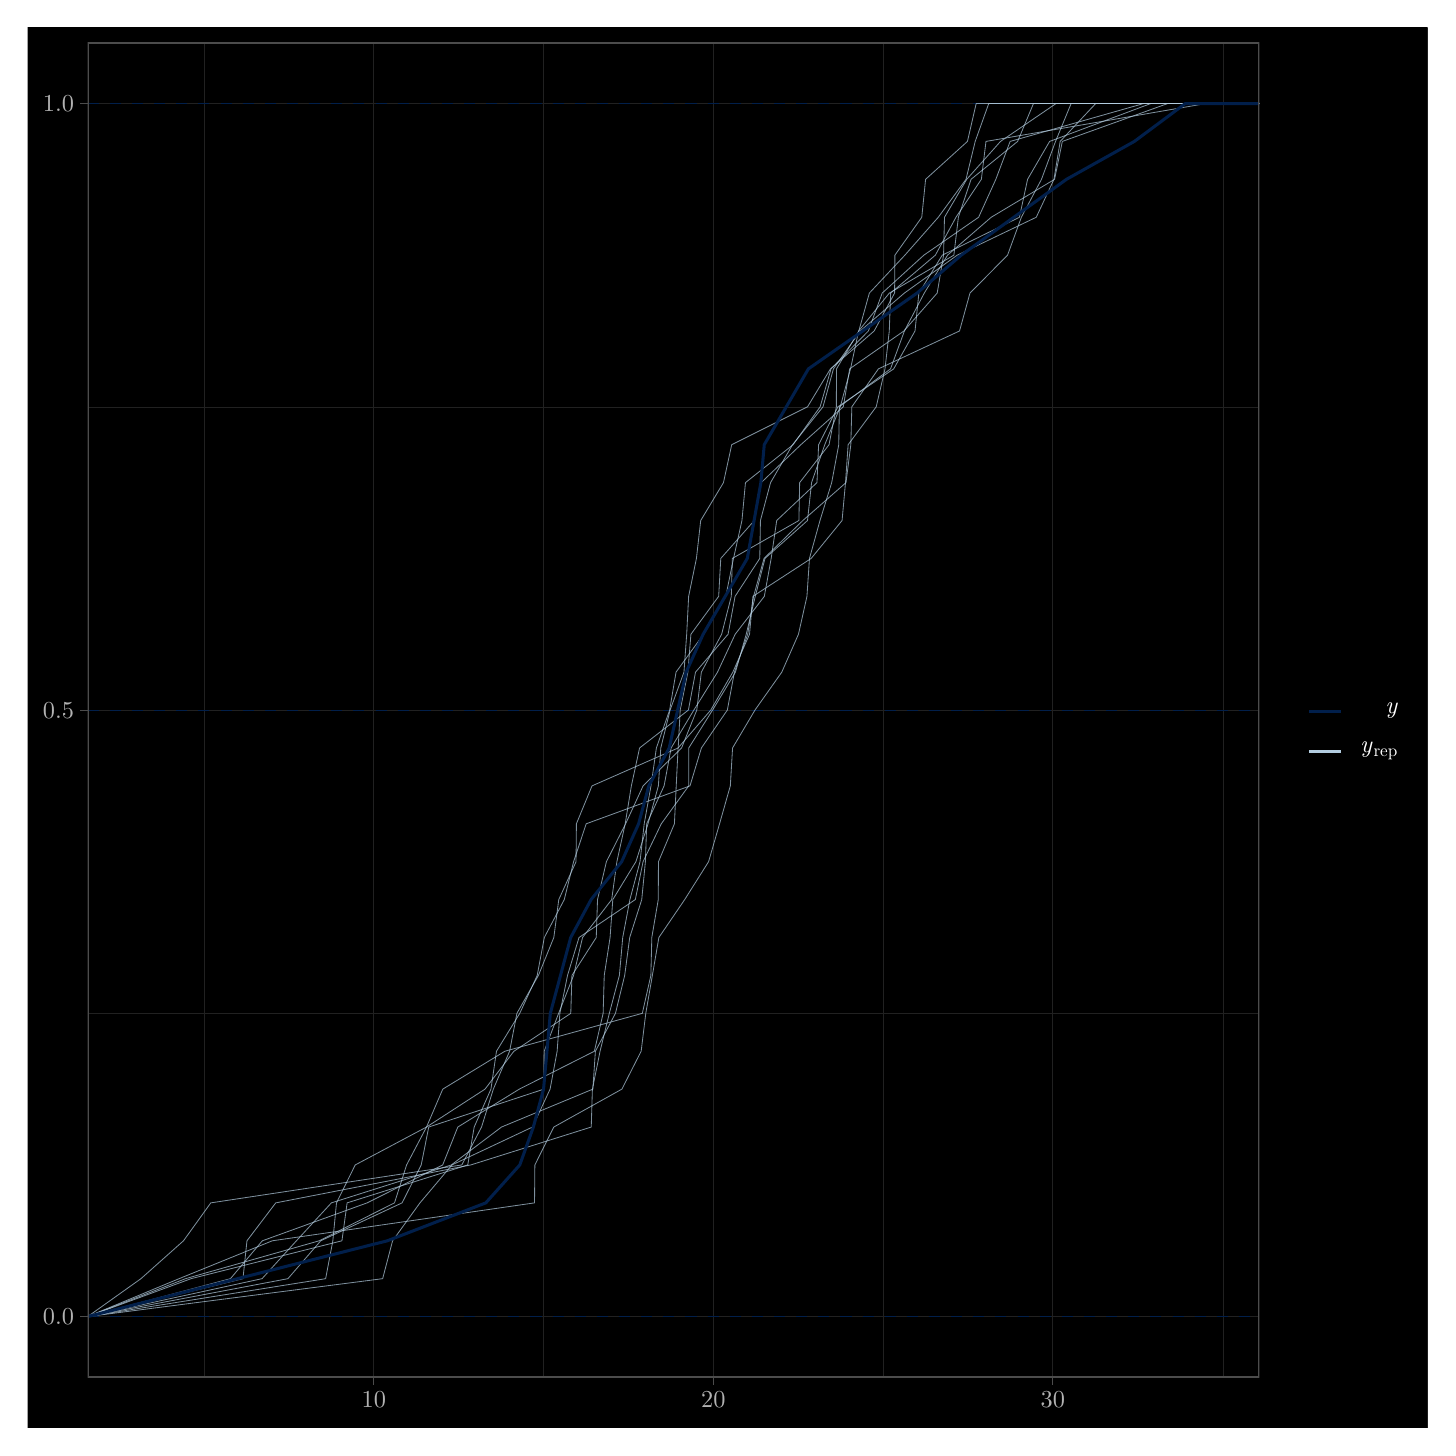
\begin{tikzpicture}[x=1pt,y=1pt]
\definecolor{fillColor}{RGB}{255,255,255}
\path[use as bounding box,fill=fillColor,fill opacity=0.00] (0,0) rectangle (505.89,505.89);
\begin{scope}
\path[clip] (  0.00,  0.00) rectangle (505.89,505.89);
\definecolor{drawColor}{RGB}{0,0,0}
\definecolor{fillColor}{RGB}{0,0,0}

\path[draw=drawColor,line width= 0.6pt,line join=round,line cap=round,fill=fillColor] (  0.00,  0.00) rectangle (505.89,505.89);
\end{scope}
\begin{scope}
\path[clip] ( 21.69, 18.22) rectangle (445.03,500.39);
\definecolor{fillColor}{RGB}{0,0,0}

\path[fill=fillColor] ( 21.69, 18.22) rectangle (445.03,500.39);
\definecolor{drawColor}{gray}{0.13}

\path[draw=drawColor,line width= 0.1pt,line join=round] ( 21.69,149.72) --
	(445.03,149.72);

\path[draw=drawColor,line width= 0.1pt,line join=round] ( 21.69,368.89) --
	(445.03,368.89);

\path[draw=drawColor,line width= 0.1pt,line join=round] ( 63.71, 18.22) --
	( 63.71,500.39);

\path[draw=drawColor,line width= 0.1pt,line join=round] (186.41, 18.22) --
	(186.41,500.39);

\path[draw=drawColor,line width= 0.1pt,line join=round] (309.11, 18.22) --
	(309.11,500.39);

\path[draw=drawColor,line width= 0.1pt,line join=round] (431.81, 18.22) --
	(431.81,500.39);

\path[draw=drawColor,line width= 0.3pt,line join=round] ( 21.69, 40.14) --
	(445.03, 40.14);

\path[draw=drawColor,line width= 0.3pt,line join=round] ( 21.69,259.31) --
	(445.03,259.31);

\path[draw=drawColor,line width= 0.3pt,line join=round] ( 21.69,478.47) --
	(445.03,478.47);

\path[draw=drawColor,line width= 0.3pt,line join=round] (125.06, 18.22) --
	(125.06,500.39);

\path[draw=drawColor,line width= 0.3pt,line join=round] (247.76, 18.22) --
	(247.76,500.39);

\path[draw=drawColor,line width= 0.3pt,line join=round] (370.46, 18.22) --
	(370.46,500.39);
\definecolor{drawColor}{RGB}{1,31,75}

\path[draw=drawColor,line width= 0.1pt,dash pattern=on 4pt off 4pt ,line join=round] ( 21.69,259.31) -- (445.03,259.31);

\path[draw=drawColor,line width= 0.2pt,dash pattern=on 4pt off 4pt ,line join=round] ( 21.69, 40.14) -- (445.03, 40.14);

\path[draw=drawColor,line width= 0.2pt,dash pattern=on 4pt off 4pt ,line join=round] ( 21.69,478.47) -- (445.03,478.47);
\definecolor{drawColor}{RGB}{179,205,224}

\path[draw=drawColor,draw opacity=0.70,line width= 0.3pt,line join=round] ( 21.69, 40.14) --
	( 57.05, 53.84) --
	(105.35, 67.53) --
	(132.55, 81.23) --
	(136.92, 94.93) --
	(144.12,108.63) --
	(149.99,122.33) --
	(172.43,136.02) --
	(222.10,149.72) --
	(225.19,163.42) --
	(225.53,177.12) --
	(227.86,190.82) --
	(227.93,204.51) --
	(233.70,218.21) --
	(234.35,231.91) --
	(235.02,245.61) --
	(246.84,259.31) --
	(254.80,273.00) --
	(260.84,286.70) --
	(262.07,300.40) --
	(283.12,314.10) --
	(294.28,327.80) --
	(295.52,341.49) --
	(296.47,355.19) --
	(306.62,368.89) --
	(309.79,382.59) --
	(311.34,396.29) --
	(311.83,409.98) --
	(327.99,423.68) --
	(335.44,437.38) --
	(344.61,451.08) --
	(346.28,464.78) --
	(425.78,478.47) --
	(445.03,478.47);

\path[draw=drawColor,draw opacity=0.70,line width= 0.3pt,line join=round] ( 21.69, 40.14) --
	( 94.04, 53.84) --
	(105.90, 67.53) --
	(135.29, 81.23) --
	(142.21, 94.93) --
	(144.92,108.63) --
	(186.54,122.33) --
	(186.64,136.02) --
	(191.86,149.72) --
	(197.26,163.42) --
	(200.50,177.12) --
	(211.03,190.82) --
	(212.91,204.51) --
	(215.91,218.21) --
	(218.14,231.91) --
	(221.11,245.61) --
	(238.75,259.31) --
	(241.32,273.00) --
	(253.09,286.70) --
	(255.62,300.40) --
	(264.54,314.10) --
	(264.78,327.80) --
	(268.44,341.49) --
	(276.38,355.19) --
	(287.39,368.89) --
	(291.16,382.59) --
	(300.84,396.29) --
	(316.79,409.98) --
	(335.89,423.68) --
	(364.45,437.38) --
	(370.84,451.08) --
	(373.09,464.78) --
	(385.93,478.47) --
	(445.03,478.47);

\path[draw=drawColor,draw opacity=0.70,line width= 0.3pt,line join=round] ( 21.69, 40.14) --
	( 77.79, 53.84) --
	( 79.24, 67.53) --
	( 89.64, 81.23) --
	(160.09, 94.93) --
	(203.64,108.63) --
	(204.06,122.33) --
	(206.83,136.02) --
	(210.18,149.72) --
	(213.81,163.42) --
	(215.02,177.12) --
	(217.61,190.82) --
	(221.27,204.51) --
	(222.78,218.21) --
	(225.23,231.91) --
	(227.18,245.61) --
	(231.97,259.31) --
	(234.28,273.00) --
	(244.22,286.70) --
	(252.26,300.40) --
	(255.06,314.10) --
	(258.10,327.80) --
	(259.37,341.49) --
	(276.57,355.19) --
	(286.36,368.89) --
	(290.29,382.59) --
	(303.79,396.29) --
	(308.78,409.98) --
	(323.83,423.68) --
	(343.62,437.38) --
	(349.84,451.08) --
	(355.00,464.78) --
	(403.27,478.47) --
	(445.03,478.47);

\path[draw=drawColor,draw opacity=0.70,line width= 0.3pt,line join=round] ( 21.69, 40.14) --
	( 40.93, 53.84) --
	( 56.31, 67.53) --
	( 66.17, 81.23) --
	(156.87, 94.93) --
	(164.00,108.63) --
	(168.26,122.33) --
	(174.14,136.02) --
	(176.79,149.72) --
	(184.56,163.42) --
	(190.12,177.12) --
	(191.91,190.82) --
	(198.15,204.51) --
	(198.28,218.21) --
	(203.92,231.91) --
	(235.06,245.61) --
	(235.79,259.31) --
	(238.56,273.00) --
	(239.66,286.70) --
	(249.69,300.40) --
	(250.45,314.10) --
	(262.57,327.80) --
	(265.04,341.49) --
	(279.38,355.19) --
	(294.72,368.89) --
	(297.02,382.59) --
	(316.63,396.29) --
	(328.65,409.98) --
	(330.95,423.68) --
	(331.29,437.38) --
	(339.32,451.08) --
	(351.53,464.78) --
	(371.60,478.47) --
	(445.03,478.47);

\path[draw=drawColor,draw opacity=0.70,line width= 0.3pt,line join=round] ( 21.69, 40.14) --
	(107.67, 53.84) --
	(110.27, 67.53) --
	(111.59, 81.23) --
	(118.35, 94.93) --
	(144.12,108.63) --
	(165.26,122.33) --
	(175.69,136.02) --
	(196.25,149.72) --
	(196.67,163.42) --
	(205.45,177.12) --
	(205.91,190.82) --
	(209.12,204.51) --
	(216.06,218.21) --
	(222.38,231.91) --
	(236.29,245.61) --
	(241.78,259.31) --
	(243.43,273.00) --
	(250.76,286.70) --
	(254.25,300.40) --
	(254.63,314.10) --
	(278.68,327.80) --
	(278.95,341.49) --
	(289.57,355.19) --
	(292.21,368.89) --
	(292.27,382.59) --
	(300.33,396.29) --
	(304.14,409.98) --
	(316.97,423.68) --
	(329.05,437.38) --
	(339.06,451.08) --
	(342.38,464.78) --
	(347.28,478.47) --
	(445.03,478.47);

\path[draw=drawColor,draw opacity=0.70,line width= 0.3pt,line join=round] ( 21.69, 40.14) --
	( 54.72, 53.84) --
	( 88.40, 67.53) --
	(183.15, 81.23) --
	(183.27, 94.93) --
	(190.11,108.63) --
	(214.72,122.33) --
	(221.68,136.02) --
	(223.35,149.72) --
	(225.73,163.42) --
	(228.08,177.12) --
	(237.41,190.82) --
	(246.04,204.51) --
	(250.01,218.21) --
	(253.90,231.91) --
	(254.71,245.61) --
	(262.81,259.31) --
	(272.49,273.00) --
	(278.52,286.70) --
	(281.59,300.40) --
	(282.50,314.10) --
	(286.30,327.80) --
	(290.53,341.49) --
	(293.08,355.19) --
	(293.30,368.89) --
	(311.79,382.59) --
	(316.81,396.29) --
	(323.98,409.98) --
	(332.39,423.68) --
	(348.17,437.38) --
	(371.06,451.08) --
	(373.87,464.78) --
	(411.95,478.47) --
	(445.03,478.47);

\path[draw=drawColor,draw opacity=0.70,line width= 0.3pt,line join=round] ( 21.69, 40.14) --
	( 59.04, 53.84) --
	(113.56, 67.53) --
	(115.43, 81.23) --
	(159.02, 94.93) --
	(161.34,108.63) --
	(167.40,122.33) --
	(169.40,136.02) --
	(177.81,149.72) --
	(184.12,163.42) --
	(186.69,177.12) --
	(193.90,190.82) --
	(197.27,204.51) --
	(201.82,218.21) --
	(239.32,231.91) --
	(243.45,245.61) --
	(252.82,259.31) --
	(255.38,273.00) --
	(260.19,286.70) --
	(262.31,300.40) --
	(266.08,314.10) --
	(280.11,327.80) --
	(295.70,341.49) --
	(297.44,355.19) --
	(297.81,368.89) --
	(307.41,382.59) --
	(336.72,396.29) --
	(340.50,409.98) --
	(354.07,423.68) --
	(359.07,437.38) --
	(366.33,451.08) --
	(371.41,464.78) --
	(377.05,478.47) --
	(445.03,478.47);

\path[draw=drawColor,draw opacity=0.70,line width= 0.3pt,line join=round] ( 21.69, 40.14) --
	( 73.27, 53.84) --
	( 84.80, 67.53) --
	(122.67, 81.23) --
	(149.97, 94.93) --
	(155.43,108.63) --
	(177.65,122.33) --
	(204.77,136.02) --
	(207.94,149.72) --
	(208.34,163.42) --
	(210.45,177.12) --
	(211.43,190.82) --
	(219.78,204.51) --
	(224.16,218.21) --
	(227.90,231.91) --
	(228.77,245.61) --
	(232.14,259.31) --
	(237.15,273.00) --
	(238.13,286.70) --
	(238.84,300.40) --
	(241.65,314.10) --
	(243.20,327.80) --
	(251.42,341.49) --
	(254.40,355.19) --
	(281.80,368.89) --
	(290.08,382.59) --
	(305.88,396.29) --
	(313.26,409.98) --
	(313.37,423.68) --
	(323.08,437.38) --
	(324.46,451.08) --
	(339.58,464.78) --
	(342.74,478.47) --
	(445.03,478.47);

\path[draw=drawColor,draw opacity=0.70,line width= 0.3pt,line join=round] ( 21.69, 40.14) --
	(128.27, 53.84) --
	(131.86, 67.53) --
	(141.75, 81.23) --
	(153.31, 94.93) --
	(182.41,108.63) --
	(188.77,122.33) --
	(191.32,136.02) --
	(192.31,149.72) --
	(195.07,163.42) --
	(199.23,177.12) --
	(219.57,190.82) --
	(222.37,204.51) --
	(228.95,218.21) --
	(238.87,231.91) --
	(238.88,245.61) --
	(247.49,259.31) --
	(255.75,273.00) --
	(259.65,286.70) --
	(262.91,300.40) --
	(266.43,314.10) --
	(281.79,327.80) --
	(283.26,341.49) --
	(288.03,355.19) --
	(293.62,368.89) --
	(297.33,382.59) --
	(300.27,396.29) --
	(311.36,409.98) --
	(334.67,423.68) --
	(336.31,437.38) --
	(340.88,451.08) --
	(357.72,464.78) --
	(363.44,478.47) --
	(445.03,478.47);

\path[draw=drawColor,draw opacity=0.70,line width= 0.3pt,line join=round] ( 21.69, 40.14) --
	( 84.69, 53.84) --
	( 97.11, 67.53) --
	(109.75, 81.23) --
	(153.08, 94.93) --
	(171.21,108.63) --
	(204.23,122.33) --
	(205.14,136.02) --
	(212.39,149.72) --
	(215.73,163.42) --
	(217.54,177.12) --
	(221.89,190.82) --
	(223.21,204.51) --
	(223.68,218.21) --
	(229.97,231.91) --
	(232.51,245.61) --
	(240.73,259.31) --
	(249.27,273.00) --
	(255.65,286.70) --
	(266.19,300.40) --
	(268.66,314.10) --
	(270.66,327.80) --
	(285.21,341.49) --
	(285.80,355.19) --
	(292.78,368.89) --
	(312.93,382.59) --
	(320.64,396.29) --
	(322.03,409.98) --
	(330.48,423.68) --
	(358.37,437.38) --
	(361.31,451.08) --
	(369.27,464.78) --
	(405.84,478.47) --
	(445.03,478.47);
\definecolor{drawColor}{RGB}{1,31,75}

\path[draw=drawColor,line width= 1.1pt,line join=round] ( 21.69, 40.14) --
	(129.97, 67.53) --
	(165.55, 81.23) --
	(177.82, 94.93) --
	(182.73,108.63) --
	(186.41,122.33) --
	(188.86,149.72) --
	(192.54,163.42) --
	(196.22,177.12) --
	(203.59,190.82) --
	(214.63,204.51) --
	(220.76,218.21) --
	(224.44,231.91) --
	(231.81,245.61) --
	(237.94,273.00) --
	(244.08,286.70) --
	(260.03,314.10) --
	(264.94,341.49) --
	(266.16,355.19) --
	(282.11,382.59) --
	(301.75,396.29) --
	(321.38,409.98) --
	(337.33,423.68) --
	(375.36,451.08) --
	(399.90,464.78) --
	(418.31,478.47) --
	(445.03,478.47);
\definecolor{drawColor}{RGB}{76,76,76}

\path[draw=drawColor,line width= 0.6pt,line join=round,line cap=round] ( 21.69, 18.22) rectangle (445.03,500.39);
\end{scope}
\begin{scope}
\path[clip] (  0.00,  0.00) rectangle (505.89,505.89);
\definecolor{drawColor}{RGB}{178,178,178}

\node[text=drawColor,anchor=base east,inner sep=0pt, outer sep=0pt, scale=  0.88] at ( 16.74, 37.11) {0.0};

\node[text=drawColor,anchor=base east,inner sep=0pt, outer sep=0pt, scale=  0.88] at ( 16.74,256.28) {0.5};

\node[text=drawColor,anchor=base east,inner sep=0pt, outer sep=0pt, scale=  0.88] at ( 16.74,475.44) {1.0};
\end{scope}
\begin{scope}
\path[clip] (  0.00,  0.00) rectangle (505.89,505.89);
\definecolor{drawColor}{RGB}{76,76,76}

\path[draw=drawColor,line width= 0.3pt,line join=round] ( 18.94, 40.14) --
	( 21.69, 40.14);

\path[draw=drawColor,line width= 0.3pt,line join=round] ( 18.94,259.31) --
	( 21.69,259.31);

\path[draw=drawColor,line width= 0.3pt,line join=round] ( 18.94,478.47) --
	( 21.69,478.47);
\end{scope}
\begin{scope}
\path[clip] (  0.00,  0.00) rectangle (505.89,505.89);
\definecolor{drawColor}{RGB}{76,76,76}

\path[draw=drawColor,line width= 0.3pt,line join=round] (125.06, 15.47) --
	(125.06, 18.22);

\path[draw=drawColor,line width= 0.3pt,line join=round] (247.76, 15.47) --
	(247.76, 18.22);

\path[draw=drawColor,line width= 0.3pt,line join=round] (370.46, 15.47) --
	(370.46, 18.22);
\end{scope}
\begin{scope}
\path[clip] (  0.00,  0.00) rectangle (505.89,505.89);
\definecolor{drawColor}{RGB}{178,178,178}

\node[text=drawColor,anchor=base,inner sep=0pt, outer sep=0pt, scale=  0.88] at (125.06,  7.21) {10};

\node[text=drawColor,anchor=base,inner sep=0pt, outer sep=0pt, scale=  0.88] at (247.76,  7.21) {20};

\node[text=drawColor,anchor=base,inner sep=0pt, outer sep=0pt, scale=  0.88] at (370.46,  7.21) {30};
\end{scope}
\begin{scope}
\path[clip] (  0.00,  0.00) rectangle (505.89,505.89);
\definecolor{fillColor}{RGB}{0,0,0}

\path[fill=fillColor] (456.03,231.74) rectangle (500.39,286.87);
\end{scope}
\begin{scope}
\path[clip] (  0.00,  0.00) rectangle (505.89,505.89);
\definecolor{fillColor}{RGB}{0,0,0}

\path[fill=fillColor] (461.53,251.70) rectangle (475.98,266.15);
\end{scope}
\begin{scope}
\path[clip] (  0.00,  0.00) rectangle (505.89,505.89);
\definecolor{drawColor}{RGB}{1,31,75}

\path[draw=drawColor,draw opacity=0.70,line width= 0.3pt,line join=round] (462.97,258.93) -- (474.53,258.93);
\end{scope}
\begin{scope}
\path[clip] (  0.00,  0.00) rectangle (505.89,505.89);
\definecolor{drawColor}{RGB}{1,31,75}

\path[draw=drawColor,line width= 1.1pt,line join=round] (462.97,258.93) -- (474.53,258.93);
\end{scope}
\begin{scope}
\path[clip] (  0.00,  0.00) rectangle (505.89,505.89);
\definecolor{fillColor}{RGB}{0,0,0}

\path[fill=fillColor] (461.53,237.24) rectangle (475.98,251.70);
\end{scope}
\begin{scope}
\path[clip] (  0.00,  0.00) rectangle (505.89,505.89);
\definecolor{drawColor}{RGB}{179,205,224}

\path[draw=drawColor,draw opacity=0.70,line width= 0.3pt,line join=round] (462.97,244.47) -- (474.53,244.47);
\end{scope}
\begin{scope}
\path[clip] (  0.00,  0.00) rectangle (505.89,505.89);
\definecolor{drawColor}{RGB}{179,205,224}

\path[draw=drawColor,line width= 1.1pt,line join=round] (462.97,244.47) -- (474.53,244.47);
\end{scope}
\begin{scope}
\path[clip] (  0.00,  0.00) rectangle (505.89,505.89);
\definecolor{drawColor}{RGB}{255,255,255}

\node[text=drawColor,anchor=base west,inner sep=0pt, outer sep=0pt, scale=  0.88] at (490.62,257.89) {\itshape y};
\end{scope}
\begin{scope}
\path[clip] (  0.00,  0.00) rectangle (505.89,505.89);
\definecolor{drawColor}{RGB}{255,255,255}

\node[text=drawColor,anchor=base west,inner sep=0pt, outer sep=0pt, scale=  0.88] at (481.48,243.84) {\itshape y};

\node[text=drawColor,anchor=base west,inner sep=0pt, outer sep=0pt, scale=  0.62] at (486.32,242.51) {r};

\node[text=drawColor,anchor=base west,inner sep=0pt, outer sep=0pt, scale=  0.62] at (488.73,242.51) {e};

\node[text=drawColor,anchor=base west,inner sep=0pt, outer sep=0pt, scale=  0.62] at (491.47,242.51) {p};
\end{scope}
\end{tikzpicture}
}
				\caption{Real versus Simulated Empirical CDFs}
			\end{figure}
		\end{column}
	\end{columns}
\end{frame}
